
\documentclass[]{./tpl/isipfe}
\graphicspath{{./img/}}
\usepackage[T1]{fontenc}
\usepackage[utf8]{inputenc}
\usepackage[hidelinks]{hyperref}
\usepackage{algorithm}
\usepackage{algorithmic}
\usepackage{float}
\usepackage{acronym}
\usepackage{textcomp}
\usepackage{enumitem}
\usepackage{rotating}
\usepackage{pdflscape}
\usepackage{comment}
\usepackage{tabularx}
\usepackage{graphicx}
\usepackage{xcolor}
\usepackage{booktabs}
\usepackage{multirow}

% Code listings — syntax highlighting
\usepackage{listings}
\lstset{
    basicstyle=\footnotesize\ttfamily,
    breaklines=true,
    breakatwhitespace=true,
    frame=single,
    numbers=left,
    numberstyle=\tiny\color{gray},
    numbersep=5pt,
    xleftmargin=15pt,
    xrightmargin=5pt,
    showstringspaces=false,
    tabsize=4,
    captionpos=b,
    keywordstyle=\color{blue}\bfseries,
    commentstyle=\color{green!60!black}\itshape,
    stringstyle=\color{red!70!black},
    backgroundcolor=\color{gray!8},
    rulecolor=\color{gray!40},
}
\lstdefinestyle{yaml}{
    language={},
    basicstyle=\footnotesize\ttfamily,
    keywordstyle=\color{blue},
    stringstyle=\color{red!70!black},
    commentstyle=\color{green!60!black},
    frame=single,
    backgroundcolor=\color{gray!8},
    breaklines=true,
}
\lstdefinestyle{bash}{
    language=bash,
    basicstyle=\footnotesize\ttfamily,
    keywordstyle=\color{blue}\bfseries,
    frame=single,
    backgroundcolor=\color{gray!8},
    breaklines=true,
}

\usepackage{tcolorbox}
\tcbuselibrary{skins,breakable}
\newtcolorbox{infobox}[1][]{
    colback=blue!5!white,
    colframe=blue!50!black,
    fonttitle=\bfseries,
    title=#1,
    breakable
}
\newtcolorbox{warningbox}[1][]{
    colback=orange!5!white,
    colframe=orange!70!black,
    fonttitle=\bfseries,
    title=#1,
    breakable
}

\usepackage{titlesec}
\input{./tpl/new_commands}
\makeindex

\begin{document}
    %============= Config new columns type ==============%
\newcolumntype{L}{>{\raggedright\arraybackslash}}
\newcolumntype{R}{>{\raggedleft\arraybackslash}}
\newcolumntype{C}{>{\centering\arraybackslash}}
%==================================================%

%========= Config the cover section ==========%

\title{Agent IA pour revue automatisée de code}

\author{Ghaith FERCHICHI}

\diplomaName{Diplôme National De Mastère Professionnel}
\speciality{Sécurité des Systèmes D'Information et des Infrastructures}

%% Encadrant professionnel
\proFramerName{Monsieur Kamel KAOUECH}
\proFramerSpeciality{Expert Infrastructure}

%% Encadrant académique
\academicFramerName{Madame Ghayet El Mouna ZHIOUA}
\academicFramerSpeciality{Maître Assistant(e)}

%% Entreprise d'accueil
\companyName{Banque de Tunisie et des Emirats}

%% Année universitaire
\collegeYear{2025-2026}

%%%%%% Signatures section %%%%%%
\proSignSentence{J'autorise l'étudiant \textbf{Ghaith FERCHICHI} à déposer son rapport de stage en vue d'une soutenance.}
\academicSignSentence{J'autorise l'étudiant \textbf{Ghaith FERCHICHI} à déposer son rapport de stage en vue d'une soutenance.}

%%% AR
\arabicAbstract{%
يصف هذا التقرير تصميم ونشر الوكيل الذكي للأمن السيبراني (\textLR{BTE Security AI Agent})، وهو أداة تعتمد منهجية \textLR{DevSecOps} لأتمتة مراجعة الأمان الخاصة بطلبات الدمج (\textLR{\textit{Pull Requests}}) على منصة \textLR{GitHub}. عند استقبال حدث خطّاف ويب (\textLR{Webhook}) والتحقق من صحته باستخدام \textLR{HMAC-SHA256}، يتم تشغيل خمس أدوات للفحص الساكن للشيفرة المصدرية بالتوازي (\textLR{Trivy} و\textLR{Gitleaks} و\textLR{Semgrep} و\textLR{Checkov} و\textLR{OSV-Scanner})، ثم تُدمج نتائجها بواسطة النموذجين \textLR{\texttt{qwen2.5-coder:7b}} و\textLR{\texttt{qwen2.5-coder:14b}} المُشغَّلين محليًا عبر \textLR{Ollama}. تُنشَر مراجعة أمنية تستند إلى معايير \textLR{OWASP Top 10}، مرفقة بدرجة للمخاطر وحكم نهائي (\textLR{\texttt{APPROVE}} أو \textLR{\texttt{REQUEST\_CHANGES}} أو \textLR{\texttt{BLOCK}}) على طلب الدمج خلال مدة تتراوح بين 15 و25 دقيقة تبعًا لدرجة تعقيده. ولا تغادر الشيفرة المصدرية البنية التحتية لبنك \textLR{BTE} في أي مرحلة من مراحل المعالجة. وتعتمد المنصة على أحد عشر حاوية \textLR{Docker} في بيئة الإنتاج، وبيئة \textLR{LocalAI} معزولة قابلة للتشغيل عند الطلب، ومساعد محادثة مزود بتسعة عشر أداة تشغيلية، إضافةً إلى طبقة متكاملة للرصد والمراقبة تعتمد على \textLR{Prometheus} و\textLR{Grafana} و\textLR{AlertManager} و\textLR{VictoriaMetrics} و\textLR{node-exporter} وتضم خمسة عشر قاعدة للتنبيه.%
}

\arabicAbstractKeywords{%
\textLR{DevSecOps}، الذكاء الاصطناعي، النماذج اللغوية المحلية، \textLR{Ollama}، \textLR{LangGraph}، \textLR{FastAPI}، \textLR{Trivy}، \textLR{Gitleaks}، \textLR{Semgrep}، \textLR{Checkov}، \textLR{OSV-Scanner}، \textLR{Prometheus}، \textLR{Grafana}، \textLR{Docker}، \textLR{GitHub Webhooks}، \textLR{OWASP}، \textLR{PostgreSQL}، \textLR{Redis}%
}

%%% FR
\frenchAbstract{%
Ce rapport décrit la conception et le déploiement du BTE Security AI Agent, un outil DevSecOps qui automatise la revue de sécurité des \textit{Pull Requests} GitHub. À la réception d'un événement webhook validé HMAC-SHA256, cinq scanners statiques (Trivy, Gitleaks, Semgrep, Checkov, OSV-Scanner) sont exécutés en parallèle ; leurs résultats sont ensuite consolidés par les modèles \texttt{qwen2.5-coder:7b} et \texttt{qwen2.5-coder:14b} servis localement par Ollama. La revue OWASP Top 10, accompagnée d'un score de risque et d'un verdict (\texttt{APPROVE}, \texttt{REQUEST\_CHANGES} ou \texttt{BLOCK}), est publiée sur la \textit{Pull Request} en 15 à 25 minutes selon sa complexité. Le code source ne quitte jamais l'infrastructure de la BTE. La plateforme s'appuie sur onze conteneurs Docker en production, une sandbox LocalAI activable à la demande, un assistant de chat doté de dix-neuf outils opérationnels, et une couche d'observabilité Prometheus, Grafana, AlertManager, VictoriaMetrics et node-exporter avec quinze règles d'alerte.%
}

\frenchAbstractKeywords{%
DevSecOps, Intelligence Artificielle, LLM Local, Ollama, LangGraph, FastAPI, Trivy, Gitleaks, Semgrep, Checkov, OSV-Scanner, Prometheus, Grafana, Docker, GitHub Webhooks, OWASP, PostgreSQL, Redis%
}

%%% EN
\englishAbstract{%
This report describes the design and deployment of the BTE Security AI Agent, a DevSecOps tool that automates the security review of GitHub \textit{Pull Requests}. When an HMAC-SHA256-validated webhook event arrives, five static scanners (Trivy, Gitleaks, Semgrep, Checkov, OSV-Scanner) run in parallel; their findings are then consolidated by the \texttt{qwen2.5-coder:7b} and \texttt{qwen2.5-coder:14b} models served locally through Ollama. The OWASP Top 10 review, together with a risk score and a verdict (\texttt{APPROVE}, \texttt{REQUEST\_CHANGES}, or \texttt{BLOCK}), is posted back to the \textit{Pull Request} in 15 to 25 minutes depending on PR complexity. Source code never leaves the BTE infrastructure. The platform relies on eleven production Docker containers, an on-demand LocalAI sandbox, a chat assistant with nineteen operational tools, and a Prometheus, Grafana, AlertManager, VictoriaMetrics and node-exporter observability layer with fifteen alert rules.%
}

\englishAbstractKeywords{%
DevSecOps, Artificial Intelligence, Local LLM, Ollama, LangGraph, FastAPI, Trivy, Gitleaks, Semgrep, Checkov, OSV-Scanner, Prometheus, Grafana, Docker, GitHub Webhooks, OWASP, PostgreSQL, Redis%
}

\setboolean{wantToTypeCompanyAddress}{true}
\companyEmail{contact@bte.com.tn}
\companyTel{71 126 000}
\companyFax{71 126 001}
\companyAddressAR{نهج بحيرة ملاران، ضفاف البحيرة، تونس}
\companyAddressFR{Rue du Lac Malaren, Les Berges du Lac, 1053 Tunis}


    \frontmatter
        \input{tpl/cover_page}
        
%===== File containing the black cover of the document ====%
%                                                          %
% Copyright (C) ISI - All Rights Reserved                  %
% Proprietary                                              %
% Written by Med Hossam <med.hossam@gmail.com>, April 2016 %
%                                                          %
% @author: HEDHILI Med Houssemeddine                       %
% @linkedin: http://tn.linkedin.com/in/medhossam           %
%==========================================================%

%== It's advised to not modify the content of this file ===%
% To set your information, go to global_config.tex file    %
%==========================================================%

\thispagestyle{cover}%
\hspace{-47pt}
\begin{minipage}[l]{0.2\columnwidth}
\vspace{6mm}

\includegraphics[width=1.1\columnwidth]{images/Logo_ISI_Black.png}\\
\end{minipage}
\hfill
\begin{minipage}[l]{0.6\columnwidth}
\centering
\footnotesize
\textbf{{MINISTERE DE L’ENSEIGNEMENT SUPERIEUR \\
ET DE LA RECHERCHE SCIENTIFIQUE}}\\
\vspace{2.5mm}
\textbf{{UNIVERSITE TUNIS EL MANAR}}\\
\vspace{2.5mm}
\textbf{{INSTITUT SUPERIEUR D’INFORMATIQUE}}
\end{minipage}
\hfill
\begin{minipage}[l]{0.02\columnwidth}
\end{minipage}
\hfill
\begin{minipage}[l]{0.18\columnwidth}
\vspace{6mm}

\includegraphics[width=0.9\columnwidth]{images/Logo_UTM_Black.png}\\
\end{minipage}
\vskip1.5cm

\begin{center}
{\LARGE{\textbf{\textsc{RAPPORT DE STAGE DE FIN D'\'ETUDES}}}}\\
\vskip0.5cm
\large

{\textbf{Présenté en vue de l'obtention du}}\\
\vskip2mm
{\textbf{\@diplomaName}}\\
{\textbf{Spécialité : \@speciality}}\\
{}
\end{center}

\begin{center}
\textrm{Par}\\
\vskip0.3cm
{\ifthenelse{\boolean{isBinomal}}
    {% IF TRUE
        \begin{center}
            \large\textbf{\@author}
        \end{center}
    }
    {\Large\textbf{\@author}}% FALSE
}
\vskip12mm

\begin{changemargin}{-9mm}{0cm}
\begin{minipage}[l]{1.1\columnwidth}
\begin{tcolorbox}[colback=white,boxrule=0pt,toprule=3pt,bottomrule=3pt,arc=0pt,top=0mm,right=0mm,left=0mm,bottom=0mm,boxsep=0.5mm]{
    \begin{tcolorbox}[colback=white, boxrule=0pt,toprule=1pt,bottomrule=1pt,arc=0pt,enlarge bottom by=-0.9mm, auto outer arc]
        \centering
        {\huge\textbf{\@title}}
    \end{tcolorbox}
}
\end{tcolorbox}
\end{minipage}
\end{changemargin}

\end{center}
\vskip8mm%

\begin{center}
\large
\begin{minipage}[c]{0.29\columnwidth}
Encadrant professionnel:\\
Encadrant académique:
\end{minipage}
%\hfill
\begin{minipage}[c]{0.45\columnwidth}
\textbf{\@proFramerName}\\
\textbf{\@academicFramerName}
\end{minipage}
\hfill
%\begin{minipage}[c]{0.26\columnwidth}
%\@proFramerSpeciality\\
%\@academicFramerSpeciality
%\end{minipage}
\end{center}
\vskip16mm

\begin{center}
\large
Réalisé au sein de \@companyName\\
\vskip0.4cm
\begin{figure}[h]
\centering
{{\fboxrule=2.5pt\fbox{
\includegraphics[width=0.4\columnwidth]{images/logo_BTE.png}}}}
\end{figure}
\end{center}

\restoregeometry
        \input{tpl/signatures}

        \setcounter{page}{1}
        \chapter*{Remerciements}

\begin{center}
\it \Large
J’adresse mes remerciements les plus sincères à toute l’équipe de la Banque de Tunisie et des Émirats, qui m’a accueilli et accompagné durant mon projet de fin d’études.\\
\vskip12mm
Je remercie tout particulièrement \textbf{\@proFramerName}, mon encadrant au sein de l’entreprise, pour ses conseils avisés et sa disponibilité tout au long du stage.\\
\vskip12mm
J’exprime aussi ma reconnaissance à \textbf{\@academicFramerName}, mon encadrante à l’ISI, dont les remarques et les orientations m’ont été d’une aide précieuse.\\
\vskip12mm
Je remercie également l’ensemble des enseignants qui m’ont accompagné durant mon cursus universitaire, pour la qualité de la formation qu’ils m’ont transmise.\\
\vskip12mm
Enfin, je remercie les membres du jury de l’honneur qu’ils me font en acceptant d’évaluer ce travail.
\end{center}
        \thispagestyle{frontmatter}

        \setcounter{secnumdepth}{3}
        \setcounter{tocdepth}{3}
        \dominitoc
        \tableofcontents
        \adjustmtc
        \thispagestyle{frontmatter}

        \listoffigures
        \thispagestyle{frontmatter}

        \listoftables
        \thispagestyle{frontmatter}

        \chapter*{Liste des abréviations}

\begingroup
\setlist[itemize]{leftmargin=0pt, itemindent=0pt, labelwidth=0pt, labelsep=0pt, label={}}
% Local override: widen the abbreviation column so long labels (e.g. DevSecOps)
% do not overlap the "=" sign.
\renewcommand{\sortitem}[2][\relax]{%
  \DTLnewrow{list}%
  \DTLnewdbentry{list}{sortlabel}{#1}%
  \DTLnewdbentry{list}{description}{%
      \begin{minipage}[t]{0.17\columnwidth}~\textbf{#1}\end{minipage}%
      \begin{minipage}[t]{0.04\columnwidth}\textbf{=}\end{minipage}%
      \begin{minipage}[t]{0.77\columnwidth}#2\end{minipage}%
  }%
}%
\begin{acronyms}

    \sortitem[AI]{
        \textbf{A}rtificial \textbf{I}ntelligence
    }
    \sortitem[API]{
        \textbf{A}pplication \textbf{P}rogramming \textbf{I}nterface
    }
    \sortitem[AVX2]{
        \textbf{A}dvanced \textbf{V}ector e\textbf{X}tensions 2
    }
    \sortitem[BCT]{
        \textbf{B}anque \textbf{C}entrale de \textbf{T}unisie
    }
    \sortitem[BTE]{
        \textbf{B}anque de \textbf{T}unisie et des \textbf{E}mirats
    }
    \sortitem[CI]{
        \textbf{C}ontinuous \textbf{I}ntegration
    }
    \sortitem[CD]{
        \textbf{C}ontinuous \textbf{D}eployment
    }
    \sortitem[CPU]{
        \textbf{C}entral \textbf{P}rocessing \textbf{U}nit
    }
    \sortitem[CVE]{
        \textbf{C}ommon \textbf{V}ulnerabilities and \textbf{E}xposures
    }
    \sortitem[DevSecOps]{
        \textbf{Dev}elopment \textbf{Sec}urity \textbf{Op}eration\textbf{s}
    }
    \sortitem[DNS]{
        \textbf{D}omain \textbf{N}ame \textbf{S}ystem
    }
    \sortitem[DSI]{
        \textbf{D}irection des \textbf{S}ystèmes d'\textbf{I}nformation
    }
    \sortitem[GGUF]{
        \textbf{GG}ML \textbf{U}niversal \textbf{F}ormat
    }
    \sortitem[GPU]{
        \textbf{G}raphics \textbf{P}rocessing \textbf{U}nit
    }
    \sortitem[HMAC]{
        \textbf{H}ash-based \textbf{M}essage \textbf{A}uthentication \textbf{C}ode
    }
    \sortitem[HTTP]{
        \textbf{H}yper\textbf{T}ext \textbf{T}ransfer \textbf{P}rotocol
    }
    \sortitem[IaC]{
        \textbf{I}nfrastructure \textbf{a}s \textbf{C}ode
    }
    \sortitem[JSON]{
        \textbf{J}ava\textbf{S}cript \textbf{O}bject \textbf{N}otation
    }
    \sortitem[LLM]{
        \textbf{L}arge \textbf{L}anguage \textbf{M}odel
    }
    \sortitem[MoE]{
        \textbf{M}ixture \textbf{o}f \textbf{E}xperts
    }
    \sortitem[NIST]{
        \textbf{N}ational \textbf{I}nstitute of \textbf{S}tandards and \textbf{T}echnology
    }
    \sortitem[NLP]{
        \textbf{N}atural \textbf{L}anguage \textbf{P}rocessing
    }
    \sortitem[OWASP]{
        \textbf{O}pen \textbf{W}eb \textbf{A}pplication \textbf{S}ecurity \textbf{P}roject
    }
    \sortitem[PR]{
        \textbf{P}ull \textbf{R}equest
    }
    \sortitem[RAM]{
        \textbf{R}andom \textbf{A}ccess \textbf{M}emory
    }
    \sortitem[REST]{
        \textbf{RE}presentational \textbf{S}tate \textbf{T}ransfer
    }
    \sortitem[RSSI]{
        \textbf{R}esponsable de la \textbf{S}écurité des \textbf{S}ystèmes d'\textbf{I}nformation
    }
    \sortitem[SAST]{
        \textbf{S}tatic \textbf{A}pplication \textbf{S}ecurity \textbf{T}esting
    }
    \sortitem[SHA]{
        \textbf{S}ecure \textbf{H}ash \textbf{A}lgorithm
    }
    \sortitem[SQL]{
        \textbf{S}tructured \textbf{Q}uery \textbf{L}anguage
    }
    \sortitem[SSH]{
        \textbf{S}ecure \textbf{Sh}ell
    }
    \sortitem[SSL]{
        \textbf{S}ecure \textbf{S}ockets \textbf{L}ayer
    }
    \sortitem[SSE]{
        \textbf{S}erver-\textbf{S}ent \textbf{E}vents
    }
    \sortitem[TTL]{
        \textbf{T}ime \textbf{T}o \textbf{L}ive
    }
    \sortitem[UI]{
        \textbf{U}ser \textbf{I}nterface
    }
    \sortitem[VPS]{
        \textbf{V}irtual \textbf{P}rivate \textbf{S}erver
    }
    \sortitem[WIP]{
        \textbf{W}ork \textbf{I}n \textbf{P}rogress
    }
    \sortitem[YAML]{
        \textbf{Y}AML \textbf{A}in't \textbf{M}arkup \textbf{L}anguage
    }
    \sortitem[OS]{
        \textbf{O}perating \textbf{S}ystem
    }

\end{acronyms}
\endgroup

        \thispagestyle{frontmatter}
        \adjustmtc

    \mainmatter
        \chapter*{Introduction générale}
\addcontentsline{toc}{chapter}{Introduction générale}
\markboth{Introduction générale}{}

Pour un établissement bancaire, la sécurité du code source est aujourd'hui un enjeu
de premier plan. La généralisation des pratiques DevOps a accéléré le rythme des
livraisons, mais elle a aussi élargi la surface d'attaque que chaque déploiement
expose. Une vulnérabilité qui franchit l'étape de fusion sans avoir été repérée peut
compromettre l'intégrité du système d'information et engager la responsabilité de la
banque, tant vis-à-vis de ses clients que de ses régulateurs. Les exemples ne manquent
pas : une injection SQL au cœur d'une API de paiement, un secret d'authentification
commité par mégarde dans un dépôt Git, ou une image Docker bâtie sur une librairie
exposée à un CVE critique. Or la revue de sécurité reste, dans le modèle classique,
un travail d'experts qui relisent chaque \textit{Pull Request} à la main. Le procédé
est lent, son résultat dépend largement du relecteur, et il passe d'autant plus mal
à l'échelle que les équipes de développement s'agrandissent.

Deux évolutions récentes rendent une autre approche envisageable. Les grands modèles
de langage (LLM) savent désormais analyser du code source et en formuler des
corrections lisibles. De leur côté, les outils d'analyse de sécurité statique (SAST)
ont gagné en maturité au point d'être exploitables en production. En les combinant,
il devient possible de déclencher une revue automatisée à chaque \textit{Pull Request} :
en quelques minutes, celle-ci produit une analyse alignée sur l'OWASP Top 10 et publie
ses commentaires de correction directement sur GitHub. C'est précisément l'objet de ce
projet de fin d'études, réalisé au sein de la Banque de Tunisie et des Emirats (BTE).
Il s'agit de concevoir et de déployer le \textbf{BTE Security AI Agent}, un moteur
DevSecOps autonome piloté par une intelligence artificielle exécutée localement.
L'agent intercepte les événements de \textit{Pull Request} GitHub, orchestre en
parallèle cinq outils d'analyse de sécurité et produit une revue complète en 15 à
25 minutes selon la complexité de la \textit{Pull Request}, sans qu'aucun
code source ne quitte l'infrastructure interne de la banque.

Le rapport s'organise en quatre chapitres. Le \textbf{premier chapitre} présente
l'organisme d'accueil et le cadre général du projet, pose la problématique et expose
la solution retenue ; il revient également sur la méthodologie Scrumban et sur le
déroulement du travail, réparti en dix sprints sur cinq mois. Le \textbf{deuxième
chapitre} pose les bases théoriques (DevSecOps, inférence locale par grands modèles
de langage, outils d'analyse statique), puis justifie les technologies retenues et
spécifie les besoins fonctionnels et non fonctionnels. Le \textbf{troisième chapitre}
détaille l'architecture logicielle : le workflow LangGraph à neuf nœuds, l'architecture
à deux modèles LLM, le schéma de la base de données et l'assistant de chat opérationnel
doté de son système anti-hallucination. Le \textbf{quatrième chapitre} décrit
l'environnement de déploiement et le travail mené phase par phase, de la configuration
des services Docker à la mise en place de l'observabilité, en passant par l'intégration
des outils de sécurité et l'implémentation du pipeline LLM. Une conclusion générale
referme le document : elle récapitule le travail accompli et trace les perspectives
d'amélioration.

        \clearpage

        \chapter{Étude préalable du sujet}

\section*{Introduction}
\addcontentsline{toc}{section}{Introduction}

Dans ce chapitre introductif, nous définissons le cadre global de notre projet.
Nous présentons d'abord l'organisme d'accueil, la Banque de Tunisie et des Emirats,
au sein de laquelle ce stage a été réalisé. Nous décrivons ensuite le processus de
revue de sécurité tel qu'il existe aujourd'hui à la BTE, avant d'en pointer les
limites et de présenter la solution proposée. Nous exposons enfin la méthodologie
adoptée, du choix du framework Agile au déroulement effectif du projet sur cinq mois.

% ─────────────────────────────────────────────────────────────────────────────
\section{Présentation de l'organisme d'accueil}

    \subsection{Présentation générale}

        La Banque de Tunisie et des Emirats (BTE) \cite{BTE} a été fondée le 10 août 1982 à la suite d'une
        convention signée entre le gouvernement tunisien et l'Abu Dhabi Investment
        Authority (ADIA). Conçue à l'origine comme banque d'investissement, elle est
        passée en 2004 au statut de banque universelle et propose désormais une gamme
        complète de produits et services financiers aux particuliers, aux professionnels
        et aux grandes entreprises. Son actionnariat binational lui donne une couverture
        forte sur les opérations de commerce international, et sa plateforme digitale
        \textbf{NEO BTE} traduit son orientation actuelle vers la modernisation des
        canaux client. Le siège social, situé au Centre Urbain Nord de Tunis, accueille
        un réseau d'agences en cours d'extension.

        Le tableau \ref{tab:bte_fiche} présente la fiche d'identité de l'établissement.

        \begin{table}[H]
        \centering
        \begin{tabular}{|m{4.5cm}|m{8.5cm}|}
        \hline
        \textbf{Dénomination} & Banque de Tunisie et des Emirats (BTE) \\
        \hline
        \textbf{Date de création} & 10 août 1982 \\
        \hline
        \textbf{Forme juridique} & Société anonyme cotée en bourse \\
        \hline
        \textbf{Actionnariat} & Partenariat entre l'État Tunisien et l'Abu Dhabi
                                Investment Authority (ADIA) \\
        \hline
        \textbf{Siège social} & Boulevard Béji Caïed Essebsi, Centre Urbain Nord,
                                1082 Tunis \\
        \hline
        \textbf{Secteur d'activité} & Banque universelle (Particuliers, Professionnels,
                                      Entreprises) \\
        \hline
        \textbf{Produits clés} & Crédits, épargne, e-banking (NEO BTE), services
                                 internationaux, leasing \\
        \hline
        \end{tabular}
        \caption{Fiche d'identité de la Banque de Tunisie et des Emirats}
        \label{tab:bte_fiche}
        \end{table}

        Dans le cadre de sa transformation numérique, la BTE a mis en place une Direction
        des Systèmes d'Information (DSI). Celle-ci est chargée d'assurer la disponibilité,
        la sécurité et l'évolution continue de ses infrastructures informatiques. Notre
        stage s'est déroulé au sein du département Informatique et Digital de cette
        direction, responsable de la modernisation des systèmes d'information et de
        la plateforme NEO BTE. La mission qui nous a été confiée est de renforcer les
        pratiques DevSecOps de l'organisation.

    \subsection{Secteur d'activité}

        L'activité de la BTE se déploie sur trois domaines qui couvrent l'ensemble des
        besoins financiers de ses clients. Le premier est la banque de détail :
        comptes courants, épargne, crédits à la consommation, cartes bancaires et packs
        dédiés (Packs Professionnels, Médecins, etc.). Le second est le financement des
        entreprises, à travers des crédits d'investissement, des lignes de crédit, des
        opérations de leasing et des services de commerce international (lettres de
        crédit, remises documentaires, transferts SWIFT) ; sur ce dernier point, la BTE
        a construit une expertise reconnue sur le marché tunisien grâce à son
        actionnariat binational. Le troisième domaine est la transformation digitale
        autour de la plateforme \textbf{NEO BTE}, qui rénove progressivement les
        interfaces client et les systèmes d'information de la banque. C'est cette
        dynamique de modernisation qui a rendu pertinent notre stage : renforcer la
        sécurité des développements logiciels en s'appuyant sur l'intelligence
        artificielle locale.

    \subsection{Organigramme}

        \begin{figure}[H]
            \centering
            \frame{
\includegraphics[width=0.85\columnwidth]{organigramme_dsi}}
            \caption{Organigramme de la Direction des Systèmes d'Information — BTE}
            \label{fig:organigramme}
        \end{figure}

        La figure \ref{fig:organigramme} présente l'organigramme de la Direction des
        Systèmes d'Information, organisée en plusieurs pôles fonctionnels : développement
        applicatif, infrastructure et réseaux, sécurité informatique et support utilisateurs.
        Notre projet de stage s'est déroulé au sein du pôle Sécurité Informatique, en
        collaboration avec les équipes de développement et d'infrastructure afin de mettre
        en place une solution DevSecOps transversale à l'ensemble de la DSI.

% ─────────────────────────────────────────────────────────────────────────────
\section{Présentation du projet}

    Le projet vise à automatiser la revue de sécurité du code à la BTE. Il associe
    pour cela de l'intelligence artificielle locale et des outils d'analyse statique. L'agent
    prend en charge l'ensemble du cycle, du déclenchement des scanners à la publication
    des commentaires de correction sur la \textit{Pull Request}, sans intervention
    humaine entre les deux. L'objectif est double : raccourcir un délai de revue qui
    dépasse aujourd'hui quarante-huit heures, et garantir qu'aucune \textit{Pull
    Request} ne soit fusionnée sans avoir été passée au crible des cinq scanners.

    \subsection{Étude de l'existant}

        Le processus de mise en production des développements logiciels à la BTE
        s'articule autour de la plateforme GitHub, qui sert à la fois de système de
        gestion de versions et d'espace de revue de code. Le cycle commence par la
        création d'une branche dédiée à partir de la branche principale du dépôt.
        Le développeur y pousse ses commits au fil de l'implémentation, puis ouvre
        une \textit{Pull Request} vers la branche cible une fois la fonctionnalité
        prête pour relecture.

        À l'ouverture de la \textit{Pull Request}, GitHub notifie l'équipe par le
        mécanisme des \textit{code owners} configuré sur les répertoires concernés.
        Selon la nature des fichiers modifiés, un développeur senior ou un référent
        sécurité prend la relecture en charge dans l'interface GitHub : examen visuel
        du diff, lecture des fichiers touchés, recoupements éventuels avec le reste
        du code base. Les remarques sont déposées sous forme de commentaires inline
        rattachés aux lignes concernées, et le dialogue avec le développeur se
        poursuit dans le fil de la \textit{Pull Request}.

        Le développeur prend en compte les retours, pousse des commits correctifs
        sur la même branche, et la \textit{Pull Request} se met automatiquement à
        jour. Une fois le code jugé prêt par le relecteur, la fusion vers la branche
        principale est déclenchée manuellement. La revue repose intégralement sur
        l'examen humain ; aucune analyse statique automatisée, aucun scanner de
        vulnérabilités et aucun \textit{gate} de pipeline ne sont greffés sur ce
        cycle. Le résultat de chaque revue est conservé dans l'historique GitHub
        de la \textit{Pull Request} concernée, accessible \textit{a posteriori} par
        l'équipe.

    \subsection{Critique de l'existant}

        L'analyse du processus existant fait apparaître plusieurs limites qui justifient
        une automatisation. Les délais de revue dépassent fréquemment quarante-huit heures,
        ce qui ralentit la livraison des fonctionnalités et laisse des vulnérabilités
        exposées plus longtemps que nécessaire. La qualité de la revue elle-même dépend
        de la disponibilité et de l'expertise du relecteur du jour : selon les
        \textit{Pull Requests}, la couverture de sécurité varie sensiblement d'un cas à
        l'autre. L'absence de \textit{gate} automatisé dans le pipeline CI/CD est sans
        doute la limite la plus directe : une \textit{Pull Request} contenant une
        vulnérabilité critique peut aujourd'hui être fusionnée sans aucun blocage
        technique. Et la gestion entièrement manuelle du processus laisse régulièrement
        passer des catégories de risques pour lesquelles l'œil humain n'est pas le bon
        outil, en particulier les secrets accidentellement commités et les dépendances
        vulnérables introduites en transitif.

        \begin{figure}[H]
            \centering
            \frame{
\includegraphics[width=\columnwidth,height=0.80\textheight,keepaspectratio]{asis_workflow}}
            \caption{Processus \textit{AS-IS} — revue manuelle de \textit{Pull
                     Request} telle qu'elle existe aujourd'hui à la BTE.}
            \label{fig:asis_workflow}
        \end{figure}



    \subsection{Solution proposée}

        \begin{figure}[H]
            \centering
            \frame{
\includegraphics[width=\textwidth]{solution_overview}}
            \caption{Vue d'ensemble de la solution BTE Security AI Agent}
            \label{fig:solution_overview}
        \end{figure}

        Face à ces défis, nous proposons le \textbf{BTE Security AI Agent}, un moteur
        d'automatisation DevSecOps piloté par l'intelligence artificielle locale, dont la
        vue d'ensemble est présentée dans la figure \ref{fig:solution_overview}. La solution
        repose sur l'interception des événements GitHub via un webhook sécurisé HMAC-SHA256,
        l'orchestration d'un workflow LangGraph à neuf nœuds, et l'utilisation de deux
        modèles de langage locaux exécutés entièrement via Ollama sur le VPS de la BTE.
        Cinq outils d'analyse s'exécutent en parallèle selon la classification de la
        \textit{Pull Request} : Trivy pour les CVE, Gitleaks pour la détection de secrets,
        Semgrep pour les failles OWASP, Checkov pour les misconfigurations d'infrastructure,
        et OSV-Scanner pour les dépendances vulnérables. Le résultat est publié directement
        sur la \textit{Pull Request} GitHub en environ 15 à 25 minutes selon la complexité
        de la PR. Cette publication comprend une revue de sécurité complète avec score de
        risque, verdict et commentaires inline accompagnés de suggestions de correction.
        La totalité de l'inférence s'exécute en local. Aucun code source ne quitte
        l'infrastructure de la BTE.

        \begin{figure}[H]
            \centering
            \frame{
\includegraphics[width=\columnwidth,height=0.85\textheight,keepaspectratio]{tobe_workflow}}
            \caption{Processus \textit{TO-BE} — revue automatisée par le BTE
                     Security AI Agent, déclenchée à chaque \textit{Pull Request}.}
            \label{fig:tobe_workflow}
        \end{figure}
% ─────────────────────────────────────────────────────────────────────────────
\section{Approche méthodologique}

    Le choix d'une méthodologie de travail conditionne directement la capacité d'un
    projet à tenir ses délais sans pour autant ignorer les imprévus qui apparaissent dès
    qu'on déploie en production. Dans notre cas, nous voulions une structure suffisamment
    cadrée pour rester lisible côté encadrement, et suffisamment souple pour absorber
    les corrections d'urgence sans casser la planification.

    \subsection{Généralités}

        Le cycle de vie d'un projet logiciel couvre l'analyse de l'existant, la
        spécification des besoins, la conception, la réalisation, les tests,
        l'exploitation et la maintenance. Plusieurs familles de méthodes encadrent ce
        cycle : le cycle en V, qui découpe le projet en phases successives ; le découpage
        en activités de type WBS ; et les méthodes Agiles, qui privilégient les
        itérations courtes et l'ajustement continu. Les méthodes classiques restent
        vulnérables à la mauvaise interprétation des besoins, aux changements
        fonctionnels en cours de route et aux dépassements de délais ; les chiffres
        régulièrement cités dans la littérature font état d'environ un quart de projets
        réussis sous ces approches \cite{Agile}, ce qui rend l'option Agile plus
        pertinente dans le contexte de notre stage.

    \subsection{Comparaison des frameworks Agile}

        Le choix de l'approche Agile étant acté, encore faut-il sélectionner le
        framework le mieux adapté à un projet d'ingénieur en solo, déployé en
        environnement de production réel, sur une durée de cinq mois avec des
        jalons d'encadrement fixés à l'avance. La famille Agile compte plusieurs
        cadres dont la philosophie diverge sensiblement. Le tableau
        \ref{tab:agile_compare} en propose une synthèse comparée sur les critères
        qui pèsent le plus dans notre contexte.

        \begin{table}[H]
        \centering
        \footnotesize
        \begin{tabular}{|m{2cm}|m{2.6cm}|m{2.6cm}|m{2.6cm}|m{2.8cm}|}
        \hline
        \textbf{Critère} & \textbf{Scrum} & \textbf{Kanban} & \textbf{XP} & \textbf{Scrumban} \\
        \hline
        Cadence
        & Sprints fixes (1 à 4 semaines)
        & Flux continu, pas de sprint
        & Itérations très courtes (1 semaine)
        & Sprints + flux Kanban interne \\
        \hline
        Planification
        & \textit{Sprint planning} avec engagement par lot
        & \textit{Pull} à la demande, aucun engagement
        & \textit{Planning game} basé sur la vélocité
        & Planning léger + \textit{pull} intra-sprint \\
        \hline
        Limites WIP
        & Implicite (taille du sprint)
        & Explicite par colonne
        & Implicite (binôme par tâche)
        & Explicite par colonne \\
        \hline
        Cérémonies
        & Daily, planning, démo, rétrospective
        & Aucune obligatoire
        & \textit{Pair programming}, TDD, refactoring constant
        & Cérémonies Scrum allégées \\
        \hline
        Rôles
        & PO, Scrum Master, équipe
        & Aucun rôle imposé
        & Coach, customer, programmer
        & Hérités de Scrum, simplifiés \\
        \hline
        Adapté solo
        & Difficile (rôles redondants)
        & Oui
        & Inadapté (\textit{pair} central)
        & Oui \\
        \hline
        Gestion imprévus
        & Faible — change le sprint en cours
        & Forte — \textit{pull} immédiat
        & Moyenne
        & Forte — classe \textit{Expedite} et WIP \\
        \hline
        Visibilité jalons
        & Forte (dates de sprint fixes)
        & Faible (flux continu)
        & Forte (\textit{releases} fréquentes)
        & Forte (sprints conservés) \\
        \hline
        \end{tabular}
        \caption{Comparaison synthétique des frameworks Agile évalués}
        \label{tab:agile_compare}
        \end{table}

        Scrum, dans sa forme canonique, suppose une équipe pluridisciplinaire avec
        des rôles distincts (Product Owner, Scrum Master, équipe de développement) ;
        ce découpage perd son sens lorsque l'équipe se réduit à une seule personne,
        et le sprint engagé devient rigide dès qu'un incident de production
        s'impose en milieu de quinzaine. \textit{eXtreme Programming} pousse plus
        loin encore les pratiques d'ingénierie (\textit{pair programming}, TDD strict,
        refactoring continu), dont l'essentiel est inopérant en solo.
        Kanban offre la souplesse maximale du flux continu, mais sacrifie la
        cadence et les jalons fixes utiles à l'encadrement académique d'un projet
        de fin d'études.

        Le \textbf{Scrumban} \cite{Ladas2009} a été retenu parce qu'il combine ce
        que Scrum et Kanban font de mieux : la cadence prévisible et les jalons de
        Scrum, couplés à la discipline de flux et aux limites WIP de Kanban. Ce
        compromis répond précisément à la double contrainte du stage : tenir un
        planning lisible pour l'encadrement aux jalons fixés à l'avance, sans pour
        autant figer la gestion quotidienne lorsqu'un incident de production
        s'invite dans le sprint en cours.

    \subsection{Adaptation de Scrumban au stage}

        Formalisée à la fin des années 2000 dans les équipes lean, la méthode
        Scrumban combine la cadence prévisible de Scrum à la discipline de flux
        propre à Kanban. Au lieu de pousser un lot de tâches au début du sprint
        et d'espérer qu'il tienne jusqu'au bout, l'équipe « tire » la prochaine
        carte dès qu'une place se libère, dans la limite imposée par le
        \textit{Work In Progress} (WIP). Le cadre obtenu garde la lisibilité du
        planning bisemestriel, utile pour l'encadrement et les jalons, tout en
        absorbant les imprévus de production sans avoir à replanifier le sprint
        en cours.

        Cette mécanique s'est imposée naturellement pour un stage d'ingénieur en
        solo, dans un environnement où les incidents arrivent rarement au moment
        où on les attend. Le rythme reste celui de Scrum \cite{Scrum} : sprints
        de deux semaines, \textit{sprint planning} en début de quinzaine, démo
        et rétrospective à la fin. Les cérémonies prévues pour les équipes
        (daily standup formel, planning poker, Scrum Master dédié) ont été
        simplifiées. La structure fondamentale a toutefois été conservée :
        backlog priorisé, sprints à durée fixe, jalons de livraison et
        définition de terminé. La figure \ref{fig:agile_scrum} illustre ce cycle.

        \begin{figure}[H]
            \centering
            \frame{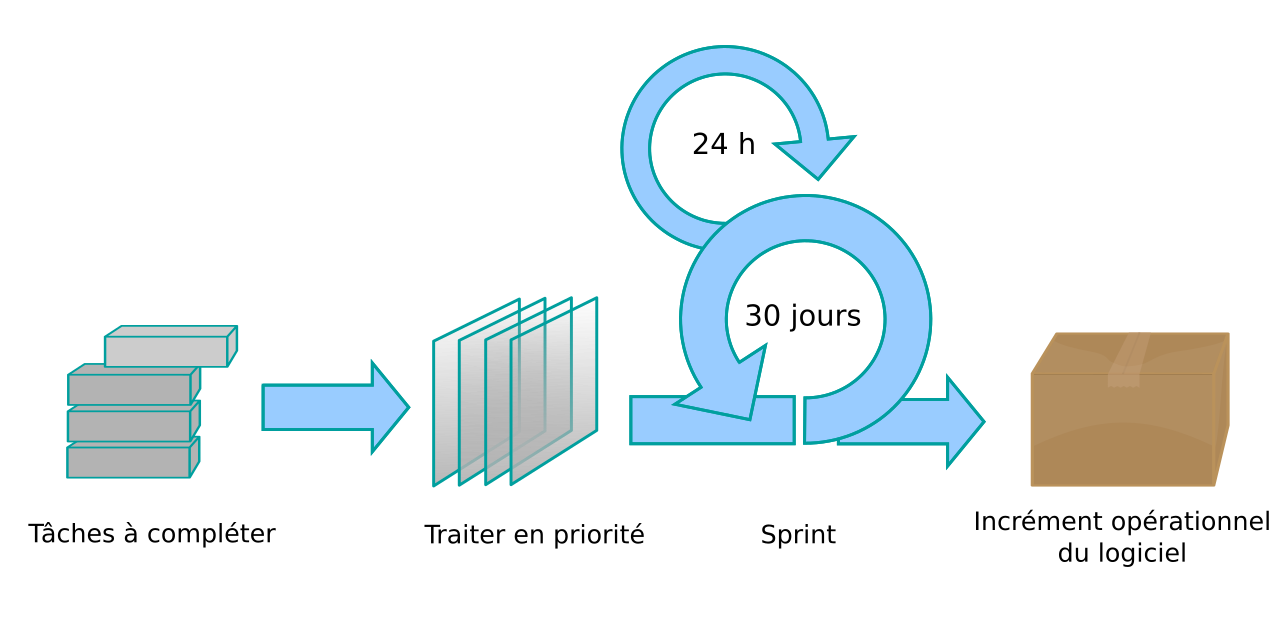
\includegraphics[width=0.82\columnwidth]{agile_scrum_cycle}}
            \caption{Cycle Scrumban adapté — sprints de deux semaines avec jalons et flux Kanban interne. \\
                     \footnotesize\textit{Source : Wikimedia Commons, CC0.}}
            \label{fig:agile_scrum}
        \end{figure}

        La gestion au jour le jour suit en revanche la logique Kanban \cite{Kanban}. Une
        seule tâche est en cours à tout moment (WIP=1), entièrement déployée et validée en
        production avant que la suivante ne démarre. La figure \ref{fig:kanban_board}
        illustre la forme générale d'un tableau de ce type, organisé en colonnes
        successives avec des plafonds par colonne.

        \begin{figure}[H]
            \centering
            \frame{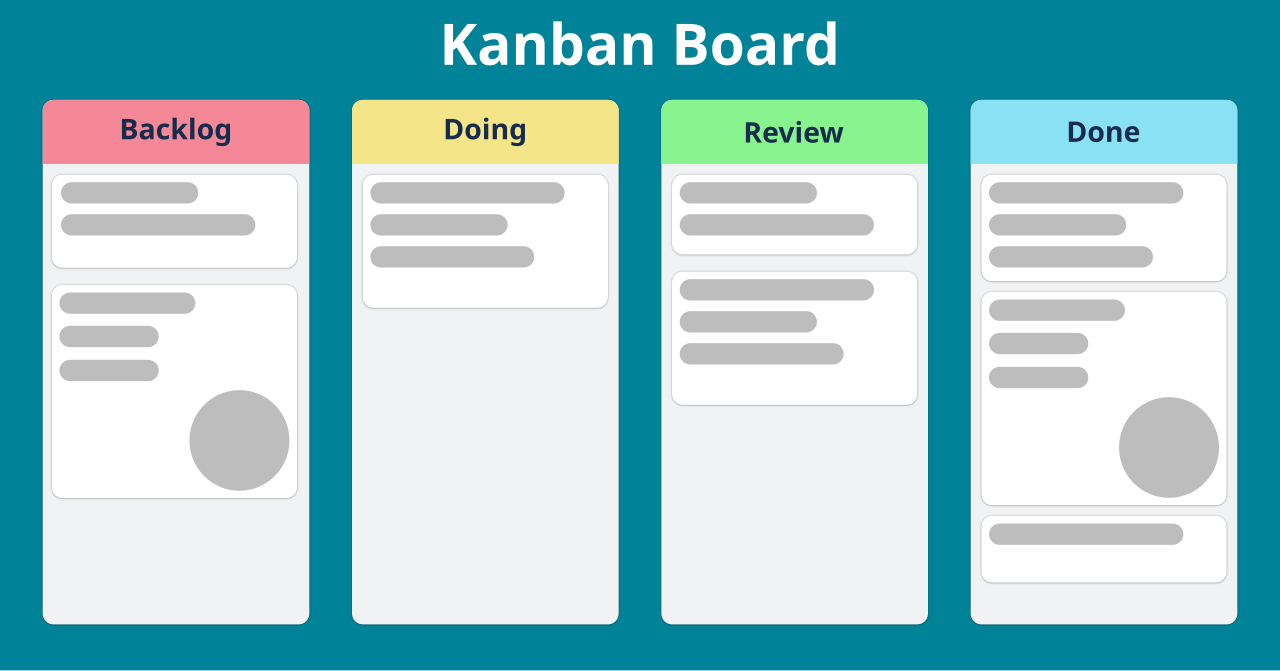
\includegraphics[width=0.88\columnwidth]{kanban_board}}
            \caption{Tableau Kanban — visualisation du flux avec limites WIP par colonne. \\
                     \footnotesize\textit{Source : Jennifer Falco, Wikimedia Commons, CC BY 4.0.}}
            \label{fig:kanban_board}
        \end{figure}

        La règle WIP=1 a un effet pratique direct : elle empêche le multitâche
        silencieux, cette dérive bien connue où plusieurs cartes traînent à 80\% sans
        qu'aucune ne franchisse la ligne d'arrivée. Elle réserve aussi une voie nette
        pour les incidents de production. Quand l'urgence disque a saturé le VPS le
        20 avril, quand AlertManager s'est révélé silencieusement cassé depuis le
        déploiement, quand VictoriaMetrics est tombée pour neuf jours, chacune de ces
        découvertes est devenue la carte prioritaire du moment. Le sprint en cours
        absorbait l'imprévu ; le sprint suivant intégrait l'amélioration durable qui
        en découlait. La structure globale du projet n'a pas eu à être revue.

    \subsection{Structure du tableau et choix des colonnes}

        Le tableau Scrumban du projet a été configuré dans Jira en partant d'un projet
        Scrum classique, auquel ont été ajoutés la fonctionnalité \textit{Kanban backlog}
        et des plafonds WIP explicites par colonne. Six colonnes composent le flux. Le
        tableau \ref{tab:scrumban_columns} récapitule leur rôle et la limite associée.

        \begin{table}[H]
        \centering
        \begin{tabular}{|m{2.2cm}|m{2.6cm}|c|m{6.4cm}|}
        \hline
        \textbf{Colonne} & \textbf{Statut Jira} & \textbf{WIP} & \textbf{Rôle} \\
        \hline
        Backlog & \texttt{To Do} & — &
            Réservoir d'idées, de dette technique et de propositions, volontairement non limité \\
        \hline
        Ready & \texttt{Ready} & 5 &
            Sprint backlog issu du \textit{sprint planning}, plafond indicatif contre le sur-engagement \\
        \hline
        In Progress & \texttt{In Progress} & \textbf{1} &
            Carte en cours de développement actif --- limite WIP=1 structurante, empêche le multitâche silencieux \\
        \hline
        In Review & \texttt{In Review} & 2 &
            Revue de code ou validation fonctionnelle avant fusion ; le plafond de 2 évite l'interruption du développement \\
        \hline
        Testing & \texttt{Testing} & 2 &
            Vérification en production sur événement réel (webhook PR, alerte Prometheus, requête chat) \\
        \hline
        Done & \texttt{Done} & — &
            Carte ayant satisfait les cinq conditions de la définition de terminé ; sinon retour en \textit{In Progress} ou \textit{Testing} \\
        \hline
        \end{tabular}
        \caption{Colonnes du tableau Scrumban et limites WIP appliquées}
        \label{tab:scrumban_columns}
        \end{table}

        Une étiquette \textbf{Expedite}, portée par les cartes d'incident de production,
        autorise une exception explicite à la limite WIP. Ce mécanisme a permis
        d'absorber les trois incidents survenus pendant le projet --- urgence disque,
        AlertManager silencieusement cassé et panne de VictoriaMetrics --- sans casser
        la planification du sprint en cours.

        \paragraph{Définition de terminé.}
        Une carte ne rejoint la colonne \textit{Done} que lorsque les cinq conditions
        suivantes sont simultanément satisfaites :
        \begin{enumerate}[label=\arabic*., leftmargin=*, itemsep=2pt]
            \item la fonctionnalité est déployée et en exécution sur le VPS de production ;
            \item les logs de l'agent restent propres après le passage du nouveau code, sans exception ni avertissement ;
            \item les métriques Prometheus reflètent son comportement lorsque cela est applicable ;
            \item elle a été déclenchée par un événement réel (webhook PR, alerte Prometheus ou requête chat) et a produit le résultat attendu ;
            \item la section correspondante de la documentation est à jour.
        \end{enumerate}
        Cette définition stricte évite que des fonctionnalités à moitié intégrées ne s'accumulent dans le système.

    \subsection{Illustration du tableau Scrumban en pratique}

        L'outil Jira a servi de support à la gestion quotidienne du tableau Scrumban
        tout au long du projet : création des cartes, suivi des transitions de
        colonne, application des limites WIP et association aux jalons. La figure
        \ref{fig:jira_sprint} présente une capture du tableau en fin de Sprint 3,
        retenu ici comme exemple représentatif de l'application concrète de la
        méthodologie. Cette capture donne à voir trois éléments structurants : la
        limite WIP=1 sur la colonne \textit{In Progress}, qui a contraint les cartes
        à être traitées une à une malgré leurs dépendances mutuelles ; les six
        colonnes du flux \textit{Backlog} $\rightarrow$ \textit{Ready}
        $\rightarrow$ \textit{In Progress} $\rightarrow$ \textit{In Review}
        $\rightarrow$ \textit{Testing} $\rightarrow$ \textit{Done} effectivement
        utilisées ; et la matérialisation du jalon M2 par une carte étiquetée
        \textit{Fixed Date}. Le détail technique du Sprint 3 lui-même --- objectif,
        obstacles rencontrés et livrable --- est documenté au chapitre 4.

        \begin{figure}[H]
            \centering
            \frame{
\includegraphics[width=\textwidth]{jira_sprint_s3}}
            \caption{Tableau Jira en fin de Sprint 3 --- application concrète
                     des règles Scrumban : WIP=1 sur \textit{In Progress},
                     flux à six colonnes et carte de jalon en classe de
                     service \textit{Fixed Date}.}
            \label{fig:jira_sprint}
        \end{figure}

    \subsection{Déroulement du projet}

        Le projet s'est déroulé sur cinq mois, du 2 février au 30 juin
        2026, structurés en dix sprints de deux semaines : huit sprints
        majeurs (Sprint~1 à Sprint~8, du 2 février au 24 mai) suivis de deux
        micro-sprints d'extension (Post-Sprint~8 et Sprint~8.1, du 25 mai au
        21 juin) consacrés à l'évaluation d'un backend
        d'inférence alternatif, à la robustesse en production et à la
        préparation de la soutenance. La rédaction du rapport a été conduite
        en parallèle des sprints 6 à 10, à raison d'une heure par jour
        bloquée en fin d'après-midi.

        Six jalons rythment cette progression et constituent les points
        d'engagement pris vis-à-vis de l'encadrement. Le jalon M1 marque
        l'existence d'un pipeline vivant, capable d'analyser une
        \textit{Pull Request} réelle de bout en bout. Le jalon M2 certifie
        l'intelligence complète du système avec les cinq scanners et la
        revue LLM publiée sur GitHub. Le jalon M3 valide l'autonomie
        opérationnelle, c'est-à-dire la capacité du système à émettre des
        alertes, à publier sur Slack et à exécuter son scheduler sans
        intervention humaine. Le jalon M4 confirme l'observabilité
        complète. Le jalon M5 atteste le durcissement de production après
        l'audit VPS et la réécriture du parser. Enfin, le jalon M6 valide
        la robustesse de la plateforme sur quatre semaines de
        fonctionnement continu, juste avant la soutenance.

        Le diagramme de Gantt de la figure \ref{fig:gantt} synthétise cette
        progression sur l'axe temporel. Les dix sprints y apparaissent sous
        forme de barres horizontales, les six jalons sous forme de losanges
        positionnés en fin de sprint correspondant, et la rédaction du
        rapport sous forme d'une bande continue chevauchant les derniers
        sprints. La lecture verticale met en évidence les transitions de
        phase, notamment le passage du développement aux micro-sprints
        d'extension entre Sprint~8 et Post-Sprint~8. La lecture horizontale
        révèle quant à elle la cadence régulière des livraisons sur
        l'ensemble de la période.

        \begin{figure}[H]
            \centering
            \frame{
\includegraphics[width=\textwidth]{gantt_chart}}
            \caption{Diagramme de Gantt du projet — dix sprints, six jalons
                     et rédaction parallèle du rapport, du 2 février
                     au 30 juin 2026.}
            \label{fig:gantt}
        \end{figure}

\section*{Conclusion}
\addcontentsline{toc}{section}{Conclusion}

Dans ce premier chapitre, nous avons présenté le contexte général du projet au sein de
la Banque de Tunisie et des Emirats, puis nous avons décrit le processus de revue de
sécurité existant et identifié ses principales limites. Cela nous a conduit à présenter
le BTE Security AI Agent comme solution à ces lacunes. Le choix méthodologique a fait
l'objet d'une comparaison entre les principaux frameworks Agile, à l'issue de laquelle
Scrumban a été retenu : sa combinaison de la cadence des sprints héritée de Scrum et
du pilotage par le flux propre à Kanban offre un cadre adapté à un projet solo de cinq
mois en environnement de production. Ce cadre apporte à la fois une visibilité sur les
jalons pour l'encadrement et une souplesse dans la gestion quotidienne lorsque les
incidents arrivent sans prévenir.

Le chapitre suivant porte sur la présentation des différentes technologies sur lesquelles
repose notre solution, avec une étude comparative entre les alternatives disponibles pour
chaque composant, ainsi que la spécification des besoins fonctionnels et non fonctionnels.

        \clearpage

        \chapter{État de l'art et choix technologiques}

\section*{Introduction}
\addcontentsline{toc}{section}{Introduction}

Ce chapitre rassemble les notions sur lesquelles notre solution s'appuie. Nous y
revenons sur le DevOps, la chaîne CI/CD et leur extension DevSecOps, sur les grands
modèles de langage et l'inférence locale, sur l'orchestration des workflows IA, ainsi
que sur les outils d'analyse de sécurité statique et la stack applicative. Une étude
comparative des technologies disponibles pour chaque composant permet ensuite de
justifier les choix retenus. Le chapitre se clôt sur la définition des besoins
fonctionnels et non fonctionnels du projet.

% ─────────────────────────────────────────────────────────────────────────────
\section{DevOps, CI/CD et DevSecOps}

    \subsection{Le DevOps}

        Le DevOps regroupe un ensemble de pratiques, d'outils et de choix culturels qui
        cherchent à raccourcir le cycle de livraison logicielle tout en gardant le produit
        stable. Il s'organise autour de trois axes : la collaboration au quotidien entre
        développement et exploitation, là où le modèle classique séparait les deux ;
        l'automatisation des tâches répétitives de la chaîne (build, tests, déploiement)
        pour limiter l'erreur humaine et libérer du temps ; et le suivi continu en
        production, qui permet de détecter rapidement les régressions et d'alimenter les
        itérations suivantes.

    \subsection{L'approche CI/CD}

        \subsubsection{Définition}

        L'approche CI/CD automatise les étapes de build, de test et de déploiement, ce
        qui raccourcit le délai entre le développement et la mise en production tout en
        réduisant les risques d'intégration \cite{DevSecOps}. Elle se décompose en deux
        phases enchaînées : l'intégration continue côté code et le déploiement continu
        côté production.

        \subsubsection{Intégration continue (CI)}

        L'intégration continue implique de modifier régulièrement le code de l'application,
        de le tester automatiquement, puis de le fusionner dans un référentiel commun. Dans
        notre projet, chaque ouverture ou mise à jour d'une \textit{Pull Request} sur GitHub
        déclenche automatiquement le pipeline de sécurité de l'agent via le mécanisme de
        webhooks.

        \subsubsection{Déploiement continu (CD)}

        Le déploiement continu automatise l'étape suivante du pipeline après l'intégration
        continue, en permettant la mise en production des modifications validées sans
        intervention manuelle. Dans notre contexte, le verdict de l'agent (APPROVE /
        REQUEST\_CHANGES / BLOCK) sert de gate de qualité et de sécurité qui conditionne
        la fusion automatique ou bloquée de la \textit{Pull Request}.

    \subsection{Du DevOps au DevSecOps}

        Le DevOps tel qu'il vient d'être décrit traite la sécurité comme une étape
        séparée, généralement repoussée à la fin du cycle. Le DevSecOps, contraction
        de Development, Security et Operations \cite{DevSecOps}, corrige cette omission
        en intégrant la sécurité à chaque étape du cycle plutôt qu'en aval
        \cite{NIST_DevSecOps}.
        L'objectif est de détecter les vulnérabilités au plus tôt, là où elles coûtent le
        moins cher à corriger ; un bug de sécurité repéré sur une \textit{Pull Request}
        avant fusion n'a presque aucun coût comparé à la même faille découverte en
        production.

        \begin{figure}[H]
            \centering
            \frame{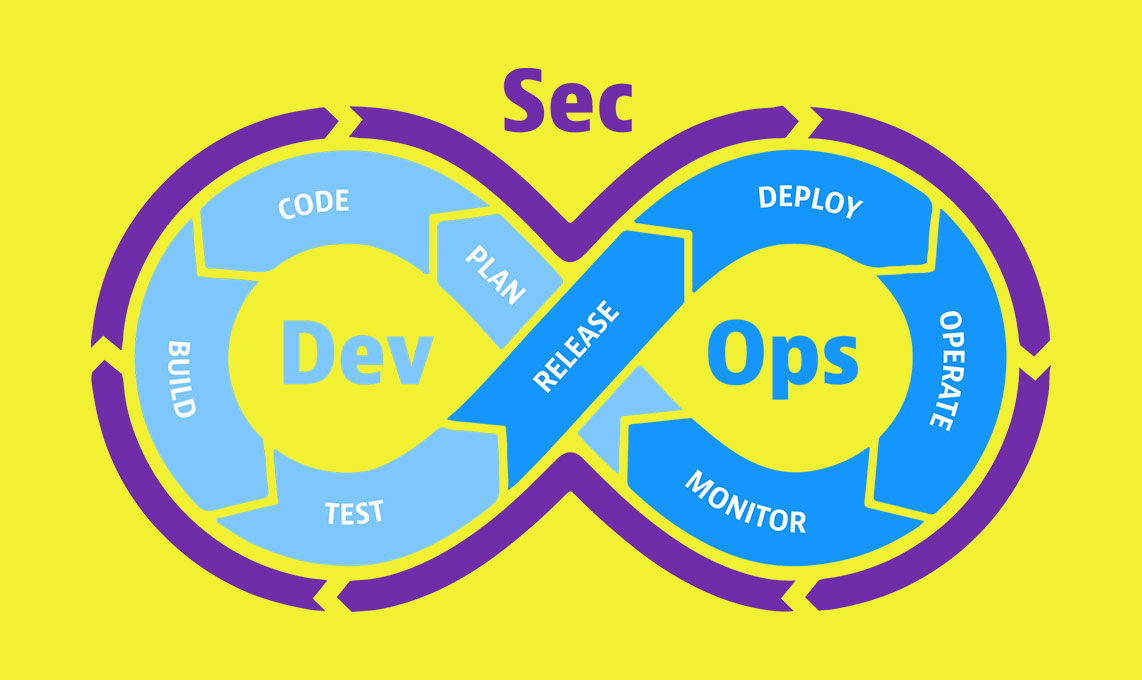
\includegraphics[width=0.82\columnwidth]{devsecops_lifecycle}}
            \caption{Cycle de vie DevSecOps — intégration de la sécurité à chaque étape. \\
                     \footnotesize\textit{Source : Rezadlt, Wikimedia Commons, CC BY-SA 4.0.}}
            \label{fig:devsecops}
        \end{figure}

        Comme le montre la figure \ref{fig:devsecops}, le DevSecOps s'organise autour de
        quelques principes structurants. Le \textit{Security as Code} consiste à exprimer
        les politiques de sécurité sous forme de code versionné et déployé automatiquement,
        au même titre qu'une configuration applicative. Le \textit{Shift Left} pousse la
        détection des vulnérabilités le plus en amont possible, idéalement sur la
        \textit{Pull Request} et avant toute fusion. Le \textit{feedback continu} complète
        l'ensemble en remontant les résultats des analyses aux développeurs concernés, sur
        leur outil de travail, dès qu'ils sont disponibles.

    \subsection{L'OWASP Top 10}

        L'OWASP (Open Web Application Security Project) publie périodiquement la liste des dix
        risques de sécurité les plus critiques pour les applications web \cite{OWASP2025}. La
        version 2025 sert de référence internationale et de grille d'analyse pour le moteur LLM
        de notre solution. Parmi les évolutions notables par rapport à la version 2021 figurent
        l'apparition de la catégorie A03:2025 --- \textit{Software Supply Chain Failures}, qui
        élargit l'ancien périmètre « composants vulnérables » à l'ensemble de la chaîne
        d'approvisionnement logicielle (dépendances, registres, pipelines CI/CD), et la nouvelle
        catégorie A10:2025 --- \textit{Mishandling of Exceptional Conditions} qui remplace SSRF.
        La catégorie A03:2025 recouvre directement le domaine couvert par OSV-Scanner et Trivy
        dans notre pipeline. Chaque finding produit par l'agent est catégorisé selon cette
        taxonomie avec une référence explicite (par exemple A01:2025 --- Broken Access Control
        ou A05:2025 --- Injection).

    \subsection{Webhooks GitHub et signature HMAC-SHA256}

        Le mécanisme concret qui relie ce cycle DevSecOps à notre agent est celui des
        \textit{webhooks} GitHub \cite{GitHubWebhooks}. À chaque ouverture ou mise à jour
        d'une \textit{Pull Request}, GitHub émet une requête HTTP POST vers l'endpoint
        public de l'agent, accompagnée d'une charge utile JSON décrivant l'événement
        (dépôt, branche, auteur, identifiant de la PR). Cet appel sortant est ce qui
        permet au pipeline de sécurité de se déclencher sans aucune action manuelle.

        Pour garantir que seul GitHub puisse déclencher le pipeline, chaque requête est
        signée par GitHub avec un secret partagé via l'algorithme HMAC-SHA256 \cite{HMAC}.
        L'agent recalcule la signature à partir de la charge utile reçue et la compare en
        temps constant à celle envoyée dans l'en-tête \texttt{X-Hub-Signature-256} : toute
        requête dont la signature ne correspond pas est rejetée en 401 avant la moindre
        opération. Ce double mécanisme associe un déclenchement automatique côté
        événement à une validation cryptographique côté réception. Il rejoint ainsi
        à la fois l'idée d'automatisation du DevOps et celle de \textit{Security as
        Code} du DevSecOps.

% ─────────────────────────────────────────────────────────────────────────────
\section{Les grands modèles de langage (LLM)}

    \subsection{Fonctionnement général}

        Les grands modèles de langage (Large Language Models, LLM) sont des réseaux de
        neurones de type Transformeur entraînés sur d'immenses corpus de texte et de code
        \cite{QwenCoder}.
        Ils sont capables de comprendre le contexte d'un fichier source et d'identifier
        des patterns de vulnérabilité connus, tels que la concaténation directe de
        chaînes dans une requête SQL ou l'utilisation de fonctions dangereuses de
        désérialisation. Ils savent également proposer des corrections dans le langage
        du développeur. Le paramètre \texttt{num\_ctx} (fenêtre de contexte) est
        critique dans notre cas. Un contexte insuffisant oblige le modèle à tronquer
        l'entrée ou à compléter depuis sa mémoire d'entraînement, ce qui produit des
        hallucinations. Nous avons calibré ce paramètre à
        12 288 tokens pour l'analyse de \textit{Pull Request} et à 6 144 tokens pour
        l'assistant de chat.

    \subsection{Inférence locale et API cloud}

        Deux paradigmes coexistent pour exécuter un LLM. L'\textbf{inférence locale}
        consiste à héberger le modèle sur l'infrastructure de l'organisation : le code
        soumis au modèle ne quitte jamais le périmètre interne, mais les performances
        dépendent du matériel disponible. L'\textbf{API cloud} consiste à invoquer un
        modèle exposé par un fournisseur tiers (OpenAI, Anthropic, etc.) : la puissance
        de calcul est déléguée, mais chaque requête transmet le code à des serveurs
        externes. Pour un établissement bancaire soumis aux exigences de confidentialité
        de la Banque Centrale de Tunisie, ce choix conditionne directement la faisabilité
        de la solution.

    \subsection{Tool calling}

        Le \textit{tool calling} (ou \textit{function calling}) désigne la capacité d'un
        LLM à émettre, en sortie, une demande structurée d'invocation d'une fonction
        externe au lieu d'une simple réponse textuelle. Le modèle reçoit en entrée la
        description d'un ensemble d'outils (nom, paramètres attendus, format de retour)
        et décide, en fonction de la requête de l'utilisateur, quel outil appeler et
        avec quels arguments. Cette capacité est exploitée par l'assistant de monitoring
        de notre solution pour interroger l'état de l'infrastructure (métriques
        Prometheus, état des conteneurs Docker, journaux applicatifs) sans que
        l'utilisateur ait à manipuler directement ces interfaces.

% ─────────────────────────────────────────────────────────────────────────────
\section{Orchestration de workflows IA}

    Un pipeline de revue de sécurité combine plusieurs étapes hétérogènes : clonage du
    dépôt, exécution parallèle de scanners, classification par un premier LLM, analyse
    approfondie par un second, publication des résultats. Coordonner ces étapes avec un
    simple script séquentiel devient rapidement intenable lorsque le pipeline doit
    partager un état entre les nœuds, router dynamiquement selon une classification,
    survivre à un redémarrage du conteneur ou s'interrompre pour une approbation humaine.

    L'orchestration de workflows IA répond à ces besoins en modélisant le pipeline sous
    forme de \textbf{graphe d'état dirigé} : chaque nœud représente une étape (souvent
    un appel LLM ou un outil), chaque arête une transition pouvant être conditionnée
    par l'état courant. Trois propriétés distinguent ce paradigme d'un script classique :
    la \textbf{persistance d'état}, qui permet de sauvegarder un \textit{checkpoint}
    après chaque nœud et de reprendre l'exécution exactement là où elle s'était arrêtée ;
    le \textbf{routage conditionnel}, qui permet à un nœud de décider du prochain en
    fonction de son résultat ; et l'\textbf{interruption humaine}, qui suspend le graphe
    en attente d'une validation externe avant de reprendre. Ces trois propriétés sont
    indispensables à notre cas d'usage, où un pipeline de 15 à 25 minutes doit survivre aux
    redémarrages et où certaines décisions critiques peuvent requérir une revue manuelle.

% ─────────────────────────────────────────────────────────────────────────────
\section{Outils d'analyse de sécurité statique (SAST)}

    \subsection{Présentation générale}

        Les outils SAST (Static Application Security Testing) analysent le code source ou
        les artefacts de build sans exécuter le programme. Aucun outil ne couvre à lui seul
        toutes les catégories de risques. Notre solution combine cinq outils complémentaires,
        chacun expert dans sa catégorie, pour assurer une couverture exhaustive. La figure
        \ref{fig:sast_overview} présente ces cinq outils et leurs domaines respectifs.

        \begin{figure}[H]
            \centering
            \frame{
\includegraphics[width=0.85\columnwidth]{sast_tools_overview}}
            \caption{Les cinq outils SAST intégrés — couverture complémentaire des risques}
            \label{fig:sast_overview}
        \end{figure}

    \subsection{Les cinq catégories de risques couvertes}

        Notre pipeline couvre cinq catégories de risques de sécurité, chacune nécessitant
        un outil spécialisé. Les \textbf{CVE images et filesystem} concernent les
        vulnérabilités connues affectant les paquets système, les bibliothèques tierces
        et les images de conteneurs utilisés par l'application. Les \textbf{secrets et
        credentials} regroupent les clés API, mots de passe, jetons d'accès et certificats
        accidentellement commités dans le dépôt. Les \textbf{vulnérabilités applicatives
        OWASP} couvrent les patterns dangereux dans le code source : injections SQL,
        désérialisation non sécurisée, chemins traversaux, etc. L'\textbf{Infrastructure-as-Code}
        désigne les erreurs de configuration dans les Dockerfile, fichiers Terraform et
        manifestes Kubernetes. Enfin, les \textbf{dépendances vulnérables} concernent les
        bibliothèques tierces déclarées dans les fichiers de dépendances
        (\texttt{requirements.txt}, \texttt{package.json}, \texttt{go.mod}, etc.) dont une
        version connue présente une faille publiée.

    \subsection{Réduction des tokens SAST}

        Les sorties brutes des scanners sont volumineuses et contiennent de nombreux champs
        redondants. Envoyer le JSON brut au LLM gaspillerait la fenêtre de contexte au
        détriment de l'analyse effective du code. Une étape de nettoyage réduit le volume
        global de 52\% avant transmission au modèle 14B, comme présenté dans le tableau
        \ref{tab:token_reduction}.

        \begin{table}[H]
        \centering
        \begin{tabular}{|m{3.5cm}|m{2.5cm}|m{2.5cm}|m{2cm}|m{3cm}|}
        \hline
        \textbf{Scanner} & \textbf{Avant} & \textbf{Après} & \textbf{Réduction} & \textbf{Technique} \\
        \hline
        Trivy (30 vulnérabilités) & \textasciitilde6 000 chars & \textasciitilde2 500 chars & 58\% & Suppression Description, CVSS, References \\
        \hline
        Gitleaks & \textasciitilde400 chars & \textasciitilde200 chars & 50\% & Champ Match omis (sécurité LLM) \\
        \hline
        Semgrep & \textasciitilde2 000 chars & \textasciitilde1 200 chars & 40\% & Findings INFO agrégés en compteur \\
        \hline
        Checkov & \textasciitilde1 500 chars & \textasciitilde800 chars & 47\% & Champ guideline URL supprimé \\
        \hline
        \textbf{Total SAST} & \textbf{\textasciitilde9 900} & \textbf{\textasciitilde4 700} & \textbf{52\%} & — \\
        \hline
        \end{tabular}
        \caption{Réduction des tokens SAST avant transmission au LLM}
        \label{tab:token_reduction}
        \end{table}

% ─────────────────────────────────────────────────────────────────────────────
\section{Stack applicative et observabilité}

    \subsection{Framework API asynchrone}

        Le cœur de l'agent expose une interface HTTP qui reçoit les webhooks GitHub,
        publie les résultats et sert l'assistant de chat en temps réel. Cette interface
        doit gérer des opérations longues (scans SAST, appels LLM de plusieurs minutes)
        sans bloquer les autres requêtes entrantes, ce qui impose un framework basé sur
        un modèle d'exécution \textbf{asynchrone} via \texttt{asyncio}. Une validation
        automatique des charges utiles entrantes est également nécessaire pour garantir
        l'intégrité des données reçues depuis les webhooks.

    \subsection{Base de données relationnelle}

        Notre architecture confie à une base de données relationnelle deux rôles distincts.
        D'une part, elle sert de \textbf{base de connaissances sécurité} pour stocker
        l'ensemble des revues de \textit{Pull Requests}, des résultats de scanners et des
        profils de risque par dépôt. Cette base alimente ainsi les requêtes de tendances.
        D'autre part, elle assure la \textbf{persistance des checkpoints} de l'orchestrateur
        de workflows. Un pipeline de 15 à 25 minutes peut ainsi survivre à un redémarrage du
        conteneur.

    \subsection{Cache et déduplication}

        Un cache en mémoire est nécessaire pour trois fonctions opérationnelles critiques.
        La \textbf{déduplication des webhooks} évite le double traitement d'un même
        événement lorsque GitHub réémet une notification après timeout. Le
        \textbf{rate limiting} garantit un maximum de pipelines simultanés par dépôt,
        protégeant le moteur d'inférence contre la surcharge. Enfin, le \textbf{cache des
        résultats de scanners} permet de retourner les résultats en quelques millisecondes
        lors d'un nouveau push sur la même branche, sans relancer une analyse complète.

    \subsection{Observabilité}

        Un système exécutant des pipelines de plusieurs minutes, dépendant d'un moteur
        d'inférence local et orchestrant cinq scanners externes, doit être instrumenté
        pour rester opérable. La stack d'observabilité couvre trois besoins distincts :
        la \textbf{collecte de métriques} (durée du pipeline, latence des appels LLM,
        taux d'erreur des scanners, occupation disque), le \textbf{stockage long terme}
        pour permettre l'analyse de tendances sur 90 jours, et la \textbf{visualisation}
        via des dashboards opérationnels. Un mécanisme d'\textbf{alerting} complète
        l'ensemble pour notifier les anomalies (saturation disque, indisponibilité du
        moteur LLM, échecs répétés de scanners) avant qu'elles n'impactent les utilisateurs.

% ─────────────────────────────────────────────────────────────────────────────
\section{Choix technologiques}

    \subsection{Choix du moteur d'inférence LLM}

        Pour un établissement bancaire, le choix entre inférence locale et API cloud est
        fortement contraint par les exigences réglementaires. Le tableau \ref{tab:ollama_vs_cloud}
        présente une comparaison entre les deux approches.

        \begin{table}[H]
        \centering
        \begin{tabular}{|m{3.5cm}|m{5cm}|m{5cm}|}
        \hline
        \textbf{Critère} & \textbf{Ollama (inférence locale)} & \textbf{API cloud (OpenAI, etc.)} \\
        \hline
        Confidentialité & Totale — code reste sur le VPS & Code transmis à des serveurs tiers \\
        \hline
        Conformité bancaire & Compatible avec les exigences de la BCT & Problématique selon la réglementation \\
        \hline
        Coût d'exploitation & Fixe — VPS existant & Variable selon le volume de tokens \\
        \hline
        Disponibilité & 100\% hors ligne & Dépend de la connectivité et du fournisseur \\
        \hline
        Contrôle de version & Modèle figé, reproductible & Version modifiée sans préavis \\
        \hline
        Latence & 3–12 tok/s sur CPU Haswell & Variable selon congestion réseau \\
        \hline
        \end{tabular}
        \caption{Comparaison entre l'inférence locale (Ollama) et les API cloud LLM}
        \label{tab:ollama_vs_cloud}
        \end{table}

        Après l'évaluation comparative présentée dans le tableau \ref{tab:ollama_vs_cloud},
        nous avons retenu Ollama \cite{Ollama} pour l'inférence locale. La confidentialité
        du code source bancaire et la conformité réglementaire vis-à-vis de la Banque
        Centrale de Tunisie imposent que les diffs de code ne quittent jamais
        l'infrastructure interne.

    \subsection{Choix du modèle LLM}

        Afin de choisir le modèle le mieux adapté à notre infrastructure (12 cœurs Intel
        Haswell AVX2, sans GPU), nous avons conduit un benchmark sur une suite de cinq
        requêtes représentatives avec le prompt système complet de 7 577 caractères. Les
        résultats sont présentés dans le tableau \ref{tab:llm_benchmark}.

        \begin{table}[H]
        \centering
        \begin{tabular}{|m{4cm}|m{1.8cm}|m{2cm}|m{2.5cm}|m{2.5cm}|}
        \hline
        \textbf{Modèle} & \textbf{Taille} & \textbf{Vitesse} & \textbf{Précision outils} & \textbf{Décision} \\
        \hline
        \texttt{qwen2.5-coder:7b} & 4,7 Go & \textasciitilde5 tok/s & 80\% & Chat (défaut) \\
        \hline
        \texttt{qwen2.5-coder:14b} & 9,0 Go & \textasciitilde3,2 tok/s & 80\% & Revue PR \\
        \hline
        \texttt{llama3.2:3b} & 2,0 Go & \textasciitilde8 tok/s & 0\% (prompt complet) & Expérimental \\
        \hline
        \texttt{granite3.1-dense:2b} & 1,6 Go & \textasciitilde8,5 tok/s & 0\% & Incompatible \\
        \hline
        \end{tabular}
        \caption{Benchmark des modèles LLM — 5 requêtes, prompt système complet, CPU BTE}
        \label{tab:llm_benchmark}
        \end{table}

        L'analyse des résultats du benchmark révèle des conclusions importantes. En premier
        lieu, \texttt{llama3.2:3b} atteint 0\% de précision avec le prompt système complet,
        car ce dernier consomme environ 2 730 tokens, occupant les deux tiers de la fenêtre
        de contexte de 4 096 tokens et ne laissant qu'un espace résiduel pour le raisonnement.
        En second lieu, \texttt{granite3.1-dense:2b} utilise le schéma propriétaire IBM
        \texttt{\{"tool\_name": ...\}}, incompatible avec notre format d'appel d'outils.
        Enfin, \texttt{qwen2.5-coder:7b} et \texttt{14b} atteignent une précision identique
        de 80\%, mais le modèle 7b est 43\% plus rapide par token. Nous retenons donc une
        architecture à deux modèles : le 7b pour la classification rapide de la
        \textit{Pull Request} (environ 30 secondes) et le 14b pour l'analyse de sécurité
        approfondie (15 à 25 minutes selon la complexité de la PR sur CPU sans GPU).

    \subsection{Choix de l'orchestrateur}

        Le tableau \ref{tab:langgraph_comp} présente une comparaison entre LangGraph
        et les alternatives d'orchestration envisagées.

        \begin{table}[H]
        \centering
        \begin{tabular}{|m{3.5cm}|m{5cm}|m{5cm}|}
        \hline
        \textbf{Critère} & \textbf{LangGraph} & \textbf{Prefect / Celery} \\
        \hline
        Persistance d'état & Native PostgreSQL (\texttt{AsyncPostgresSaver}) & Implémentation custom requise \\
        \hline
        Reprise après crash & Automatique depuis le checkpoint & Partielle selon configuration \\
        \hline
        Interruption humaine & \texttt{interrupt\_before} natif & Complexe à implémenter \\
        \hline
        Routage conditionnel & Arêtes conditionnelles natives & Nécessite des contournements \\
        \hline
        Intégration LLM & LangChain native & Non native \\
        \hline
        \end{tabular}
        \caption{Comparaison entre LangGraph et les alternatives d'orchestration}
        \label{tab:langgraph_comp}
        \end{table}

        Après l'évaluation présentée dans le tableau \ref{tab:langgraph_comp}, nous avons
        choisi LangGraph \cite{LangGraph}, bibliothèque Python construite sur LangChain
        \cite{LangChain}. Sa persistance d'état native sur PostgreSQL garantit qu'un
        pipeline de 15 à 25 minutes survit aux redémarrages du conteneur et reprend exactement
        là où il s'était arrêté. Il s'agit d'une exigence fondamentale pour notre cas
        d'usage.

    \subsection{Choix des outils SAST}

        Le tableau \ref{tab:sast_comp} présente la comparaison effectuée pour le choix de
        chaque outil selon sa catégorie de risque.

        \begin{table}[H]
        \centering
        \begin{tabular}{|m{2.3cm}|m{2cm}|m{4.5cm}|m{3cm}|}
        \hline
        \textbf{Catégorie} & \textbf{Retenu} & \textbf{Justification} & \textbf{Rejeté} \\
        \hline
        CVE images \& filesystem & Trivy & Léger, JSON structuré, base CVE quotidienne & Grype (moins mature) \\
        \hline
        Secrets \& credentials & Gitleaks & 130+ règles, champ \texttt{Match} omettable & TruffleHog (plus lent) \\
        \hline
        SAST OWASP & Semgrep & Règles OWASP épinglées, déterministe & SonarQube (serveur dédié) \\
        \hline
        Infrastructure-as-Code & Checkov & pip-installable, Dockerfile + Terraform & KICS (moins de règles) \\
        \hline
        Dépendances & OSV-Scanner & Base Google OSV, aucune clé API & Snyk (fonctionnalités payantes) \\
        \hline
        \end{tabular}
        \caption{Étude comparative des outils SAST par catégorie de risque}
        \label{tab:sast_comp}
        \end{table}

        Après évaluation des alternatives, la combinaison Trivy \cite{Trivy} + Gitleaks
        \cite{Gitleaks} + Semgrep \cite{Semgrep} + Checkov \cite{Checkov} + OSV-Scanner
        \cite{OSVScanner} offre la couverture la plus exhaustive, avec des formats de
        sortie JSON homogènes facilitant le nettoyage et la réduction des tokens avant
        transmission au LLM.

    \subsection{Choix de la stack applicative}

        Pour le framework API, nous retenons \textbf{FastAPI} \cite{FastAPI}, framework
        Python ASGI haute performance basé sur les annotations de type Python 3.10+.
        Sa gestion native de l'asynchronisme via \texttt{asyncio} est essentielle pour
        exécuter des sous-processus de scanning et des appels LLM en parallèle sans
        bloquer le thread principal. Il assure également une validation automatique des
        payloads via Pydantic. Cette validation préserve l'intégrité des données reçues
        depuis les webhooks GitHub.

        Pour la base de données relationnelle, nous retenons \textbf{PostgreSQL}
        \cite{PostgreSQL}, qui assume les deux rôles décrits précédemment : la base de
        connaissances sécurité et la persistance des checkpoints LangGraph via
        l'\texttt{AsyncPostgresSaver}. Son écosystème mature et son support natif des
        types JSON facilitent le stockage des résultats hétérogènes des scanners.

        Pour le cache et la déduplication, nous retenons \textbf{Redis} \cite{Redis}.
        Son opération atomique \texttt{SET NX} permet une déduplication fiable des
        webhooks, et sa gestion native des TTL convient parfaitement au cache des
        résultats de scanners (TTL d'une heure) et au rate limiting (maximum trois
        pipelines simultanés par dépôt).

    \subsection{Choix de la stack d'observabilité}

        Le tableau \ref{tab:obs_stack} présente les composants de la stack d'observabilité
        et les alternatives considérées.

        \begin{table}[H]
        \centering
        \begin{tabular}{|m{3cm}|m{4cm}|m{5cm}|}
        \hline
        \textbf{Composant} & \textbf{Rôle} & \textbf{Alternative rejetée} \\
        \hline
        Prometheus \cite{Prometheus} & Collecte de métriques, 15 règles d'alerte & DataDog (cloud externe, coût) \\
        \hline
        VictoriaMetrics \cite{VictoriaMetrics} & Stockage long terme 90 jours & InfluxDB (déploiement plus complexe) \\
        \hline
        Grafana \cite{Grafana} & 3 dashboards de visualisation & Kibana (orienté logs, pas métriques) \\
        \hline
        node-exporter \cite{NodeExporter} & Métriques host réelles depuis \texttt{/host/proc} & cAdvisor (namespace Docker uniquement) \\
        \hline
        AlertManager \cite{AlertManager} & Routage alertes → agent → Slack & PagerDuty (payant, cloud) \\
        \hline
        \end{tabular}
        \caption{Stack d'observabilité et alternatives rejetées}
        \label{tab:obs_stack}
        \end{table}

        La combinaison \textbf{Prometheus + VictoriaMetrics + Grafana + node-exporter +
        AlertManager} a été retenue. C'est d'abord la seule pile entièrement open source
        et auto-hébergeable qui couvre les quatre besoins, ce qui prolonge la contrainte
        de confidentialité déjà appliquée au moteur LLM. Les cinq composants ont par
        ailleurs été conçus pour s'intégrer entre eux sans adaptateur. Prometheus émet
        vers AlertManager nativement et Grafana lit indifféremment Prometheus et
        VictoriaMetrics, ce qui nous a évité d'écrire des couches de pontage. Reste le
        cas particulier de \texttt{node-exporter} \cite{NodeExporter} : sur un VPS qui
        utilise le \textit{containerd snapshotter}, c'était la seule option capable
        d'exposer les vraies métriques de l'hôte, cAdvisor \cite{cAdvisor} restant
        aveugle au noyau sous-jacent.

    \subsection{Synthèse des choix technologiques}

        Le tableau \ref{tab:tech_synthesis} récapitule l'ensemble des choix technologiques
        effectués pour notre solution.

        \begin{table}[H]
        \centering
        \begin{tabular}{|m{5cm}|m{4cm}|m{3.5cm}|}
        \hline
        \textbf{Besoin} & \textbf{Technologie retenue} & \textbf{Version} \\
        \hline
        Framework API async & FastAPI & 0.135+ \\
        \hline
        Orchestration workflow IA & LangGraph & 1.1+ \\
        \hline
        Inférence LLM locale & Ollama & latest \\
        \hline
        Modèle de classification & \texttt{qwen2.5-coder:7b} & 4,7 Go \\
        \hline
        Modèle d'analyse sécurité & \texttt{qwen2.5-coder:14b} & 9,0 Go \\
        \hline
        Base de données & PostgreSQL & 16-alpine \\
        \hline
        Cache / Déduplication & Redis & 7-alpine \\
        \hline
        CVE scanning & Trivy & 0.69+ \\
        \hline
        Détection de secrets & Gitleaks & 8.30+ \\
        \hline
        SAST OWASP & Semgrep & 1.157+ \\
        \hline
        IaC scanning & Checkov & 3.2.517+ \\
        \hline
        Dépendances vulnérables & OSV-Scanner & 2.3+ \\
        \hline
        Métriques & Prometheus + VictoriaMetrics & latest \\
        \hline
        Dashboards & Grafana & latest \\
        \hline
        Métriques host & node-exporter & latest \\
        \hline
        Reverse proxy & Nginx & alpine \\
        \hline
        Conteneurisation & Docker + Compose & 29.4.0 \\
        \hline
        \end{tabular}
        \caption{Tableau de synthèse des choix technologiques}
        \label{tab:tech_synthesis}
        \end{table}

% ─────────────────────────────────────────────────────────────────────────────
\section{Analyse et définition des besoins}

    \subsection{Besoins fonctionnels}

        La plateforme couvre cinq fonctions principales, qui suivent le parcours naturel
        d'une \textit{Pull Request} depuis son ouverture jusqu'à son archivage.

        La première est la \textbf{détection automatisée des vulnérabilités} : à l'ouverture
        ou à la mise à jour d'une PR, l'agent clone le dépôt et lance en parallèle les
        scanners retenus pour la classification observée. Sur cette base, il produit une
        \textbf{revue de sécurité combinée} en un unique appel au modèle 14B, structurée en
        quatre éléments : analyse OWASP Top 10, score de risque
        (\textsc{info} → \textsc{critical}), verdict
        (\textsc{approve} / \textsc{request\_changes} / \textsc{block}) et commentaires
        \textit{inline} porteurs de suggestions de correction. Le résultat est ensuite
        \textbf{publié sur GitHub} sous trois formes : un commentaire global dans
        l'onglet \textit{Conversation}, des commentaires \textit{inline} dans l'onglet
        \textit{Files Changed} et un statut de commit positionné pour servir de
        \textit{gate} au CI/CD. Une fois la PR clôturée, la revue, les sorties brutes des scanners et la
        liste des fichiers touchés sont \textbf{persistés dans PostgreSQL}, ce qui alimente
        les analyses de tendance par dépôt et les requêtes ultérieures depuis le chat.
        Cette dernière fonction est précisément le \textbf{chat opérationnel en temps réel} :
        servi en SSE, il pilote dix-neuf outils qui couvrent l'hôte, Docker, Ollama, Redis,
        Prometheus, PostgreSQL et les artefacts SAST.

    \subsection{Besoins non fonctionnels}

        Au-delà des fonctionnalités elles-mêmes, plusieurs contraintes pèsent sur la
        qualité de service attendue de la plateforme.

        La contrainte la plus structurante est la \textbf{confidentialité} : la totalité
        de l'inférence LLM doit s'exécuter en local, sans qu'aucun code source ni diff
        ne quitte l'infrastructure BTE. Il s'agit de la condition de conformité
        réglementaire imposée par le secteur bancaire. Vient ensuite la \textbf{performance} : le
        pipeline complet, de la réception du webhook à la publication de la revue, doit
        tenir en 15 à 25 minutes selon la complexité de la \textit{Pull Request} pour ne pas
        peser sur les cycles de livraison. La
        \textbf{résilience} et la \textbf{fiabilité} sont deux exigences proches mais
        distinctes. La première impose que le système continue à fonctionner si un
        scanner ou le modèle LLM devient temporairement injoignable, ce que prennent en
        charge le circuit breaker et les fallbacks. La seconde impose qu'un pipeline en
        cours d'exécution survive à un redémarrage du conteneur, ce qui repose sur la
        persistance des checkpoints LangGraph dans PostgreSQL. L'\textbf{observabilité}
        demande que toutes les métriques critiques (durée du pipeline, taux d'erreur,
        usage disque, état d'Ollama) remontent à Prometheus et soient consultables dans
        Grafana. Enfin, la \textbf{sécurité de la plateforme elle-même} couvre trois
        points concrets : signature HMAC-SHA256 des webhooks, authentification sur les
        interfaces exposées, et exclusion des secrets détectés par Gitleaks du payload
        envoyé au LLM.

\section*{Conclusion}
\addcontentsline{toc}{section}{Conclusion}

Ce chapitre a posé les bases conceptuelles du projet. Nous avons revisité le DevOps,
la CI/CD et leur extension DevSecOps qui intègre la sécurité à chaque étape du cycle ;
puis le fonctionnement des grands modèles de langage et l'enjeu particulier de
l'inférence locale dans un contexte bancaire ; enfin les principes d'orchestration de
workflows IA et les cinq familles de risques couvertes par les outils SAST. L'étude
comparative qui a suivi a fixé les choix technologiques retenus : Ollama \cite{Ollama}
pour la confidentialité bancaire, LangGraph \cite{LangGraph} pour la persistance native
de l'état, et l'assemblage Trivy / Gitleaks / Semgrep / Checkov / OSV-Scanner pour la
couverture SAST. Les besoins fonctionnels et non fonctionnels recensés en fin de
chapitre cadrent la conception détaillée du chapitre suivant.

        \clearpage

        \chapter{Conception de la solution}

\section*{Introduction}
\addcontentsline{toc}{section}{Introduction}

Ce chapitre décrit la conception architecturale du BTE Security AI Agent. Il part de la
vue globale de l'architecture logicielle, de ses onze conteneurs et de son point
d'entrée, pour entrer ensuite dans la conception de chacun des six sous-systèmes qui
composent la solution : l'inférence LLM, la revue de \textit{Pull Request}, l'analyse du
diff, l'assistant de chat opérationnel, la persistance et l'observabilité.

% ─────────────────────────────────────────────────────────────────────────────
\section{Présentation de l'architecture logicielle}

    \subsection{Architecture en couches}

        La plateforme BTE Security AI Agent est déployée sous forme de onze conteneurs
        Docker organisés en quatre couches fonctionnelles complémentaires. La figure
        \ref{fig:full_arch} présente cette architecture globale avec l'ensemble des
        interactions entre les composants.

        \begin{figure}[H]
            \centering
            \frame{
\includegraphics[width=\textwidth]{full_architecture}}
            \caption{Architecture globale du BTE Security AI Agent}
            \label{fig:full_arch}
        \end{figure}

        La \textbf{couche entrée} est assurée par nginx \cite{NGINX} en tant que reverse
        proxy et unique point d'entrée externe sur les ports 80 et 443. Il achemine les
        requêtes vers les services internes selon le chemin URL et applique une
        authentification HTTP Basic sur les interfaces sensibles. La \textbf{couche IA}
        comprend le FastAPI \cite{FastAPI} agent, qui orchestre le workflow LangGraph
        \cite{LangGraph}, appelle les modèles LLM et exécute les scanners, Ollama
        \cite{Ollama}, le serveur d'inférence LLM accessible uniquement depuis le réseau
        Docker \cite{Docker} interne, et Open WebUI qui offre une interface graphique
        complémentaire pour interagir directement avec les modèles Ollama lors des phases
        de mise au point. La \textbf{couche données} est constituée de
        PostgreSQL \cite{PostgreSQL}, qui héberge la base de connaissances sécurité et les
        checkpoints LangGraph, et de Redis \cite{Redis}, qui assure la déduplication des
        webhooks, le rate limiting et le cache des résultats de scanners. Enfin, la
        \textbf{couche observabilité} regroupe Prometheus \cite{Prometheus},
        VictoriaMetrics \cite{VictoriaMetrics}, Grafana \cite{Grafana},
        node-exporter \cite{NodeExporter} et AlertManager \cite{AlertManager}, qui
        assurent la collecte, le stockage, la visualisation et l'alerting.

    \subsection{Inventaire des conteneurs}

        Le tableau \ref{tab:containers} présente l'inventaire détaillé des onze conteneurs
        avec leurs caractéristiques principales.

        \begin{table}[H]
        \centering
        \begin{tabular}{|m{3.5cm}|m{3cm}|m{2cm}|m{2cm}|m{2.5cm}|}
        \hline
        \textbf{Conteneur} & \textbf{Image} & \textbf{Port} & \textbf{RAM} & \textbf{Rôle} \\
        \hline
        \texttt{devsecops-agent} & Python 3.12 custom & 8000 & \textasciitilde120 Mo & Cœur IA + API \\
        \hline
        \texttt{ollama} & \texttt{ollama/\allowbreak{}ollama:latest} & interne & \textasciitilde10 Go & Inférence LLM \\
        \hline
        \texttt{postgres} & \texttt{postgres:16-alpine} & interne & \textasciitilde33 Mo & BD + checkpoints \\
        \hline
        \texttt{redis} & \texttt{redis:7-alpine} & interne & \textasciitilde5 Mo & Cache + dédup \\
        \hline
        \texttt{nginx} & \texttt{nginx:alpine} & 80, 443 & \textasciitilde3 Mo & Reverse proxy \\
        \hline
        \texttt{prometheus} & \texttt{prom/\allowbreak{}prometheus} & interne & \textasciitilde26 Mo & Métriques \\
        \hline
        \texttt{alertmanager} & \texttt{prom/\allowbreak{}alertmanager} & interne & \textasciitilde10 Mo & Routage alertes \\
        \hline
        \texttt{grafana} & \texttt{grafana/\allowbreak{}grafana} & interne & \textasciitilde96 Mo & Dashboards \\
        \hline
        \texttt{victoriametrics} & \texttt{victoria-metrics} & interne & \textasciitilde97 Mo & Stockage 90j \\
        \hline
        \texttt{node-exporter} & \texttt{prom/\allowbreak{}node-exporter} & \texttt{host:9100} & \textasciitilde10 Mo & Métriques host \\
        \hline
        \texttt{open-webui} & \texttt{open-webui:main} & 3001 & \textasciitilde300 Mo & UI Ollama \\
        \hline
        \end{tabular}
        \caption{Inventaire des 11 conteneurs — ports, mémoire et rôles}
        \label{tab:containers}
        \end{table}

    \subsection{Routage et point d'entrée}

        Nginx est le point d'entrée unique de la plateforme. Le tableau
        \ref{tab:nginx_routing} présente l'ensemble des règles de routage configurées.

        \begin{table}[H]
        \centering
        \begin{tabular}{|m{3.5cm}|m{3.5cm}|m{2cm}|m{2cm}|}
        \hline
        \textbf{Location} & \textbf{Upstream} & \textbf{Timeout} & \textbf{Auth} \\
        \hline
        \texttt{GET /} & redirect → \texttt{/ui} & — & — \\
        \hline
        \texttt{GET /ui} & \texttt{agent:8000/ui} & défaut & Basic Auth \\
        \hline
        \texttt{POST /chat/} & \texttt{agent:8000/chat/} & 1800s & Basic Auth \\
        \hline
        \texttt{POST /\allowbreak{}webhooks/\allowbreak{}github} & \texttt{agent:8000} & 30s & HMAC \\
        \hline
        \texttt{/grafana/} & \texttt{grafana:3000} & défaut & Grafana auth \\
        \hline
        \texttt{/\allowbreak{}prometheus/} & \texttt{prometheus:9090} & défaut & — \\
        \hline
        \end{tabular}
        \caption{Table de routage nginx}
        \label{tab:nginx_routing}
        \end{table}

% ─────────────────────────────────────────────────────────────────────────────
\section{Description de la conception du logiciel}

    \subsection{Sous-système d'inférence LLM}

        \subsubsection{Architecture logique}

        La séparation du pipeline LLM en deux modèles distincts répond à une contrainte de
        performance. Utiliser le modèle 14B pour la classification de la
        \textit{Pull Request} serait disproportionné : cette tâche ne nécessite que la
        production d'une simple étiquette JSON en environ trente secondes, alors que la revue de
        sécurité approfondie requiert un modèle plus capable. La figure
        \ref{fig:two_model_arch} illustre cette architecture.

        \begin{figure}[H]
            \centering
            \frame{
\includegraphics[width=0.9\columnwidth]{two_model_architecture}}
            \caption{Architecture à deux modèles LLM}
            \label{fig:two_model_arch}
        \end{figure}

        Les instances LLM sont construites une seule fois par processus, puis réutilisées
        pour les appels suivants. La configuration \texttt{OLLAMA\_\allowbreak{}MAX\_\allowbreak{}LOADED\_\allowbreak{}MODELS=1}
        garantit en outre qu'un seul modèle est chargé en RAM à la fois, ce qui réserve
        l'ensemble des ressources au modèle actif.

        La fusion de deux appels 14B séquentiels en un seul appel combiné dans le nœud
        \texttt{analyze\_\allowbreak{}review\_\allowbreak{}node} est l'optimisation principale du pipeline. Avant
        cette optimisation, l'analyse de sécurité et la revue de qualité de code nécessitaient
        deux appels successifs totalisant entre trente et cinquante minutes. Après la fusion,
        un seul appel produit les deux résultats en quinze à vingt-cinq minutes
        selon la complexité de la \textit{Pull Request} (mesure empirique sur CPU
        Haswell 12 cœurs sans GPU), soit un gain de près de cinquante pourcent
        sur la durée totale.

        \paragraph{Contrainte matérielle.}
        La durée d'analyse de 15 à 25 minutes par \textit{Pull Request} découle directement
        du choix d'inférence locale sur CPU sans GPU, imposé par les exigences de
        confidentialité de la BCT. Sur ce matériel, le modèle 14B produit environ 3 tokens
        par seconde. Une migration vers un GPU dédié, qui resterait sur l'infrastructure BTE
        et préserverait donc cette confidentialité, ramènerait l'analyse à quelques minutes
        par \textit{Pull Request} ; cette perspective est développée dans la conclusion
        générale.

        \subsubsection{Configuration des fabriques LLM}

        Le tableau \ref{tab:llm_factories} détaille la configuration de chaque fonction de
        fabrique LLM utilisée dans le pipeline.

        \begin{table}[H]
        \centering
        \begin{tabular}{|m{3.5cm}|m{2cm}|m{2cm}|m{2cm}|m{2cm}|m{2.5cm}|}
        \hline
        \textbf{Fonction} & \textbf{Modèle} & \textbf{num\_ctx} & \textbf{num\_predict} & \textbf{temp.} & \textbf{Durée} \\
        \hline
        \texttt{get\_\allowbreak{}fast\_\allowbreak{}llm()} & 7b & 4 096 & 512 & 0.0 & \textasciitilde30s \\
        \hline
        \texttt{get\_\allowbreak{}combined\_\allowbreak{}llm()} & 14b & 12 288 & 2 500 & 0.1 & 15–25 min \\
        \hline
        \end{tabular}
        \caption{Configuration des fonctions de fabrique LLM}
        \label{tab:llm_factories}
        \end{table}

    \subsection{Sous-système de revue de Pull Request}

        \subsubsection{Architecture logique}

        Le workflow de revue de \textit{Pull Request} est modélisé comme un
        \texttt{StateGraph} LangGraph \cite{LangGraph} avec neuf nœuds et un état partagé
        de type TypedDict nommé \texttt{PRReviewState}. La figure \ref{fig:langgraph_graph}
        présente la topologie complète du graphe.

        \begin{figure}[H]
            \centering
            \frame{
\includegraphics[width=\columnwidth,height=0.80\textheight,keepaspectratio]{langgraph_state_graph}}
            \caption{Graphe d'état LangGraph}
            \label{fig:langgraph_graph}
        \end{figure}

        L'\texttt{intake\_node} est le point d'entrée du workflow. Il assure la
        déduplication Redis avec l'opération \texttt{SET NX}, le rate limiting, le clone
        shallow du dépôt avec token injecté dans l'URL, la génération du diff local avec
        quinze lignes de contexte via \texttt{git diff -U15}, et la récupération des
        dix dernières revues du dépôt depuis PostgreSQL pour injection dans le prompt. Le
        \texttt{classify\_\allowbreak{}node} appelle ensuite le modèle 7B avec \texttt{format="json"}
        et \texttt{temperature=0.\allowbreak{}0} pour classifier la PR en cinq catégories : feature,
        dependency, infrastructure, config et docs. En cas d'indisponibilité du LLM, le
        circuit breaker active le fallback regex \texttt{\_\allowbreak{}fallback\_\allowbreak{}classify()} basé sur
        les extensions de fichiers.

        Les nœuds de scanning, à savoir \texttt{scan\_\allowbreak{}full\_\allowbreak{}node} et \texttt{scan\_\allowbreak{}fs\_\allowbreak{}node},
        exécutent les scanners applicables en parallèle via \texttt{asyncio.\allowbreak{}gather()},
        avec isolation des erreurs par coroutine. Si un scanner échoue, le pipeline
        continue avec les autres. Chaque résultat est mis en cache dans Redis avec un TTL
        d'une heure. L'\texttt{analyze\_\allowbreak{}review\_\allowbreak{}node} est le cœur du pipeline. Il envoie
        au modèle 14B le diff annoté avec numéros de lignes, les résultats nettoyés des
        scanners et le prompt combiné. Il extrait ensuite par regex le JSON tail contenant
        le score de risque, le verdict et les commentaires inline. Le \texttt{report\_node}
        finalise le traitement en publiant la revue sur GitHub, en fixant le statut du
        commit et en sauvegardant un fichier \texttt{summary.\allowbreak{}json} dans les artefacts.

        Le tableau \ref{tab:scan_matrix} présente la matrice de sélection des scanners selon
        la classification de la \textit{Pull Request}. Trivy FS et Gitleaks s'exécutent
        systématiquement pour toutes les catégories sauf docs. Les scanners additionnels
        sont activés selon la classification.

        \begin{table}[H]
        \centering
        \begin{tabular}{|m{3cm}|c|c|c|c|c|}
        \hline
        \textbf{Classification} & \textbf{Trivy FS} & \textbf{Gitleaks} & \textbf{Semgrep} & \textbf{Checkov} & \textbf{OSV} \\
        \hline
        \texttt{feature} & \checkmark & \checkmark & \checkmark & & \\
        \hline
        \texttt{dependency} & \checkmark & \checkmark & & & \checkmark \\
        \hline
        \texttt{infrastructure} & \checkmark & \checkmark & & \checkmark & \\
        \hline
        \texttt{config} & \checkmark & \checkmark & & & \\
        \hline
        \texttt{docs} & & & & & \\
        \hline
        \end{tabular}
        \caption{Matrice de sélection des scanners selon la classification de la PR}
        \label{tab:scan_matrix}
        \end{table}

        Lorsqu'un Dockerfile est détecté dans la \textit{Pull Request}, le nœud
        \texttt{scan\_\allowbreak{}full\_\allowbreak{}node} est activé à la place de \texttt{scan\_\allowbreak{}fs\_\allowbreak{}node}. Dans
        ce cas, l'image Docker est construite puis scannée par Trivy en complément du scan
        du filesystem.

        La catégorie \texttt{config} ne déclenche pour sa part ni Checkov ni OSV-Scanner.
        Checkov est réservé à la classification \texttt{infrastructure}, qui couvre les
        Dockerfile et les manifestes Terraform ou Kubernetes, alors qu'un simple fichier de
        configuration applicatif ne relève pas de l'Infrastructure-as-Code ; Trivy FS et
        Gitleaks y suffisent à couvrir respectivement les CVE de filesystem et les secrets
        éventuels.

        Deux fonctions de routage guident le flux du graphe. La fonction \texttt{route\_scans}
        redirige vers \texttt{skip\_\allowbreak{}scan\_\allowbreak{}node} pour les PRs de documentation, vers
        \texttt{scan\_\allowbreak{}full\_\allowbreak{}node} si un Dockerfile est détecté, et vers \texttt{scan\_\allowbreak{}fs\_\allowbreak{}node}
        dans tous les autres cas. La fonction \texttt{route\_risk} redirige vers
        \texttt{escalate\_\allowbreak{}node} lorsque le score de risque est CRITICAL ou HIGH et que
        l'escalade Slack est activée, et vers \texttt{report\_node} dans tous les autres cas.
        Tout nœud qui lève une exception positionne \texttt{state["error"]} et déclenche
        le routage vers \texttt{error\_node}.

        \subsubsection{Diagramme d'interaction — Réception du webhook}

        La figure \ref{fig:inter_webhook} présente le flux d'interaction entre GitHub,
        nginx, l'agent FastAPI et Redis lors de la réception d'un événement
        \textit{Pull Request}. L'agent valide d'abord la signature HMAC-SHA256, vérifie
        l'absence de doublon dans Redis, puis lance le pipeline LangGraph en tâche de fond
        et retourne immédiatement un code 202 à GitHub.

        \begin{figure}[H]
            \centering
            \frame{
\includegraphics[width=0.88\columnwidth]{inter_webhook}}
            \caption{Diagramme d'interaction — Réception et validation du webhook GitHub}
            \label{fig:inter_webhook}
        \end{figure}

        \subsubsection{Diagramme d'interaction — Pipeline de revue}

        La figure \ref{fig:inter_pipeline} illustre la séquence d'interactions entre
        les nœuds LangGraph, Ollama, les outils SAST et l'API GitHub lors du traitement
        complet d'une \textit{Pull Request}. Le modèle 7B est d'abord interrogé pour la
        classification, puis les scanners s'exécutent en parallèle, et enfin le modèle
        14B produit la revue combinée qui est publiée sur GitHub.

        \begin{figure}[H]
            \centering
            \frame{\includegraphics[width=\textwidth]{inter_pipeline}}
            \caption{Diagramme d'interaction — Pipeline LangGraph de revue de sécurité}
            \label{fig:inter_pipeline}
        \end{figure}

    \subsection{Sous-système d'analyse du diff}

        \subsubsection{Architecture logique}

        Un modèle de langage peut halluciner des numéros de lignes qui n'existent pas dans
        le diff réel de la \textit{Pull Request}. Or, poster un commentaire \textit{inline}
        sur une ligne inexistante provoque une erreur 422 de l'API GitHub. Le module
        \texttt{diff\_\allowbreak{}parser.\allowbreak{}py} résout ce problème en construisant, pour chaque fichier
        modifié, l'ensemble exact des numéros de lignes valides avant toute publication.

        \begin{figure}[H]
            \centering
            \frame{
\includegraphics[width=\columnwidth,height=0.78\textheight,keepaspectratio]{diff_parser_state_machine}}
            \caption{Machine à états du diff parser}
            \label{fig:diff_parser}
        \end{figure}

        Comme le montre la figure \ref{fig:diff_parser}, le parser parcourt le diff ligne
        par ligne et reconstruit, pour chaque fichier modifié, l'ensemble des numéros de
        lignes réellement présents dans la nouvelle version : les lignes ajoutées et les
        lignes de contexte alimentent cet ensemble, tandis que les lignes supprimées sont
        ignorées puisqu'elles n'existent pas dans le fichier final. Tout commentaire du
        modèle portant sur une ligne absente de cet ensemble est écarté avant publication,
        ce qui supprime les hallucinations de numéros de lignes.

        \subsubsection{Format du diff annoté}

        En plus du diff brut utilisé pour le récit de sécurité, un diff annoté de numéros
        de lignes visibles est transmis au modèle. Cette annotation lui permet de cibler
        précisément les lignes problématiques dans ses commentaires \textit{inline}. La
        figure \ref{fig:annotated_diff} illustre ce format.

        \begin{figure}[H]
            \centering
            \frame{
\includegraphics[width=0.82\columnwidth]{annotated_diff_format}}
            \caption{Format du diff annoté avec numéros de lignes transmis au modèle 14B}
            \label{fig:annotated_diff}
        \end{figure}

    \subsection{Sous-système d'assistant de chat opérationnel}

        \subsubsection{Architecture logique}

        L'assistant de chat BTE Security AI Agent utilise une boucle ReAct
        (Reasoning + Acting) personnalisée. Cette conception est rendue nécessaire par le
        fait que \texttt{qwen2.\allowbreak{}5-coder} produit les appels d'outils en JSON texte brut
        et non via l'API native d'Ollama. La figure \ref{fig:react_loop_arch} illustre
        le flux complet de cette boucle.

        \begin{figure}[H]
            \centering
            \frame{
\includegraphics[width=\columnwidth,height=0.80\textheight,keepaspectratio]{react_loop_architecture}}
            \caption{Boucle ReAct personnalisée}
            \label{fig:react_loop_arch}
        \end{figure}

        À chaque tour, les tokens produits par le modèle sont accumulés et analysés pour y
        détecter un appel d'outil au format JSON, qu'un extracteur tolérant sait reconnaître
        sous plusieurs formes (objet direct, bloc délimité, JSON embarqué dans du texte).
        Deux gardes encadrent la boucle : la première bloque tout appel identique déjà
        effectué dans la même réponse, ce qui supprime les boucles infinies ; la seconde
        force un appel d'outil dès qu'une question porte sur une donnée en temps réel (CPU,
        disque, conteneurs, alertes), pour empêcher le modèle d'y répondre de mémoire.
        L'outil est ensuite exécuté et son résultat injecté dans le contexte. La boucle se
        répète jusqu'à huit appels au maximum, après quoi la réponse finale est diffusée en
        événements SSE.

        Un modèle de langage a tendance à inventer des valeurs de métriques (pourcentage de
        CPU, espace disque libre, nombre de conteneurs) lorsqu'il répond à des questions sur
        l'état de l'infrastructure. Six couches de protection ont été conçues pour éliminer
        complètement ce comportement, comme présenté dans la figure
        \ref{fig:anti_hallucination_layers}.

        \begin{figure}[H]
            \centering
            \frame{
\includegraphics[width=0.85\columnwidth]{anti_hallucination_layers}}
            \caption{Système anti-hallucination}
            \label{fig:anti_hallucination_layers}
        \end{figure}

        Les trois premières couches agissent sur la configuration du modèle :
        \texttt{temperature=0.\allowbreak{}0} rend la génération déterministe et supprime toute
        invention probabiliste de valeurs ; \texttt{num\_ctx} porté à 6 144 tokens laisse
        environ 4 100 tokens libres pour les observations des outils ; et
        \texttt{num\_predict} plafonné à 800 tokens garantit des réponses complètes. Les trois
        suivantes relèvent du contrôle applicatif : la garde sans-outil déjà évoquée, un bloc
        ANTI-HALLUCINATION de cinq règles dans le prompt système, et l'injection, après chaque
        appel d'outil, d'une observation imposant que toute valeur citée apparaisse verbatim
        dans un bloc \texttt{[OBSERVATION]}.

        L'assistant dispose de dix-neuf outils de monitoring couvrant l'ensemble de
        l'infrastructure. Le tableau \ref{tab:tools} présente ces outils organisés par
        catégorie.

        \begin{table}[H]
        \centering
        \begin{tabular}{|m{2.5cm}|m{5cm}|m{5.5cm}|}
        \hline
        \textbf{Catégorie} & \textbf{Outils} & \textbf{Données retournées} \\
        \hline
        VPS / Host & \texttt{vps\_status}, \texttt{disk\_usage}, \texttt{top\_\allowbreak{}processes}, \texttt{network\_\allowbreak{}stats}, \texttt{system\_\allowbreak{}net\_\allowbreak{}io} & CPU, RAM, disque, processus, interfaces réseau \\
        \hline
        Docker & \texttt{list\_\allowbreak{}containers}, \texttt{container\_\allowbreak{}logs}, \texttt{container\_\allowbreak{}stats}, \texttt{inspect\_\allowbreak{}container}, \texttt{list\_images}, \texttt{restart\_\allowbreak{}service} & État, logs, CPU/RAM live, santé \\
        \hline
        Ollama & \texttt{ollama\_\allowbreak{}status} & Modèles chargés, RAM consommée \\
        \hline
        Prometheus & \texttt{query\_\allowbreak{}prometheus}, \texttt{query\_\allowbreak{}prometheus\_\allowbreak{}range}, \texttt{prometheus\_\allowbreak{}alerts} & Métriques, tendances, alertes actives \\
        \hline
        Redis & \texttt{redis\_info} & Mémoire, hit rate, clients \\
        \hline
        Artifacts & \texttt{list\_\allowbreak{}scan\_\allowbreak{}artifacts}, \texttt{read\_\allowbreak{}scan\_\allowbreak{}artifact} & Fichiers SAST par PR \\
        \hline
        Base de données & \texttt{query\_\allowbreak{}database} & SELECT lecture seule \\
        \hline
        \end{tabular}
        \caption{Les 19 outils de monitoring du chat opérationnel}
        \label{tab:tools}
        \end{table}

        \subsubsection{Diagramme d'interaction — Boucle ReAct}

        La figure \ref{fig:inter_react} décrit le cycle d'interaction entre l'utilisateur,
        le serveur SSE, le modèle LLM et les outils de monitoring lors d'une question
        portant sur l'état de l'infrastructure. Le modèle génère un appel d'outil, l'agent
        l'exécute et injecte le résultat comme observation, puis le modèle produit la
        réponse finale en citant uniquement les valeurs présentes dans l'observation.

        \begin{figure}[H]
            \centering
            \frame{
\includegraphics[width=0.88\columnwidth]{inter_react}}
            \caption{Diagramme d'interaction — Boucle ReAct du chat opérationnel}
            \label{fig:inter_react}
        \end{figure}

    \subsection{Sous-système de persistance}

        \subsubsection{Architecture logique}

        La base de données PostgreSQL comprend six tables applicatives, auxquelles s'ajoutent
        les quatre tables créées automatiquement par LangGraph pour la persistance des
        checkpoints. La figure \ref{fig:db_er} présente le diagramme entité-association
        de l'ensemble des tables applicatives.

        \begin{figure}[H]
            \centering
            \frame{
\includegraphics[width=0.88\columnwidth]{database_er_diagram}}
            \caption{Diagramme E-A de la base de données PostgreSQL}
            \label{fig:db_er}
        \end{figure}

        \subsubsection{Description des tables}

        La table \texttt{pr\_reviews} est la table centrale de la base de connaissances.
        Elle conserve, pour chaque revue de \textit{Pull Request}, ses métadonnées (dépôt,
        numéro, auteur, classification), le score de risque et le verdict, le texte complet
        de la revue ainsi que le résumé des scanners et la liste des fichiers modifiés. La table
        \texttt{scan\_\allowbreak{}results} enregistre les sorties brutes de chaque scanner par dépôt et
        par déclencheur. La table \texttt{repo\_\allowbreak{}profiles} maintient un score de risque moyen
        glissant et un compteur de revues par dépôt, mis à jour après chaque exécution du
        nœud d'analyse. La table \texttt{security\_\allowbreak{}policies} contient les politiques de
        sécurité qui définissent les seuils de blocage, par exemple zéro CVE critique
        autorisé ou obligation de scan des secrets. La table \texttt{sbom\_cache} met en
        cache le Software Bill of Materials par dépôt pour éviter de rescanner les
        dépendances inchangées. Enfin, la table \texttt{incidents} permet de tracer les
        incidents de sécurité détectés via le chat ou les alertes.

        Les quatre tables LangGraph (\texttt{checkpoints}, \texttt{checkpoint\_\allowbreak{}blobs},
        \texttt{checkpoint\_\allowbreak{}writes} et \texttt{checkpoint\_\allowbreak{}migrations}) sont créées
        automatiquement par le checkpointer au démarrage de l'application. Elles contiennent
        l'état complet du graphe sérialisé et permettent la reprise automatique du pipeline
        après tout redémarrage du conteneur.

    \subsection{Sous-système d'observabilité}

        \subsubsection{Architecture logique}

        La stack d'observabilité centralise la surveillance de la plateforme. La figure
        \ref{fig:monitoring_stack} présente le flux de métriques depuis les sources de collecte
        jusqu'aux dashboards Grafana et aux alertes Slack.

        \begin{figure}[H]
            \centering
            \frame{
\includegraphics[width=0.88\columnwidth]{monitoring_stack}}
            \caption{Architecture de la stack d'observabilité}
            \label{fig:monitoring_stack}
        \end{figure}

        L'agent expose vingt-huit métriques Prometheus personnalisées à l'endpoint
        \texttt{/metrics}, en plus des métriques HTTP auto-instrumentées. Treize couvrent
        l'agent, Ollama et le disque ; les quinze autres, ajoutées lors de l'extension
        d'observabilité décrite au chapitre suivant, se répartissent en trois familles :
        des métriques par conteneur (mémoire, CPU, trafic réseau, état), émises par un
        \textit{poller} interrogeant le socket Docker toutes les trente secondes ; des
        métriques de santé pour la sandbox LocalAI ; et une télémétrie A/B du routeur de
        chat, labellisée par couple \texttt{backend} et \texttt{model} afin de comparer
        Ollama et LocalAI sur les mêmes requêtes.

        La métrique \texttt{ollama\_\allowbreak{}reachable}, mise à jour toutes les trente secondes par
        un \textit{poller} asynchrone, distingue deux états qu'une simple jauge de modèles
        chargés confond : Ollama inactif entre deux revues, qui est l'état normal, et Ollama
        réellement injoignable. Cette distinction évite les fausses alertes critiques pendant
        les périodes de veille.

        Les quinze règles d'alerte sont organisées en cinq groupes : \textit{disk} (quatre
        règles sur l'occupation disque, côté node-exporter et côté agent), \textit{host}
        (trois règles : CPU, mémoire, I/O disque), \textit{agent} (trois règles :
        disponibilité, taux d'erreur, \textit{backlog} de revues), \textit{ollama} (deux
        règles : joignabilité et durée sans modèle chargé) et \textit{localai} (trois règles
        \texttt{info} sur la sandbox optionnelle). Une règle d'inhibition dans AlertManager
        supprime les alertes LocalAI redondantes lorsque la sandbox est arrêtée volontairement.

\section*{Conclusion}
\addcontentsline{toc}{section}{Conclusion}

Ce chapitre a couvert la conception complète du BTE Security AI Agent. L'architecture
globale repose sur onze conteneurs Docker organisés en quatre couches, exposés derrière
un unique point d'entrée nginx. La conception logicielle a ensuite été détaillée
sous-système par sous-système : l'inférence LLM à deux modèles, le pipeline LangGraph
à neuf nœuds piloté par des arêtes conditionnelles selon la classification de la PR,
le parser de diff qui élimine les hallucinations de numéros de lignes, l'assistant de
chat ReAct protégé par six couches anti-hallucination et ses dix-neuf outils de
monitoring, la base PostgreSQL à six tables applicatives, et la stack d'observabilité
étendue à vingt-huit métriques personnalisées. Chaque sous-système a suivi le même
plan : architecture logique, puis diagramme d'interaction. La concrétisation de ces
décisions, sprint par sprint, fait l'objet du chapitre suivant.

        \clearpage

        \chapter{Réalisation et résultats}

\section*{Introduction}
\addcontentsline{toc}{section}{Introduction}

Ce chapitre rend compte de la réalisation effective du projet sur le VPS de la BTE.
Il s'ouvre sur la description de l'environnement matériel et logiciel sur lequel la
plateforme a été déployée, puis enchaîne sur l'implémentation sprint par sprint
selon la méthodologie Scrumban introduite au chapitre 1. Chaque sprint suit le même
gabarit (objectif inscrit au backlog, obstacles rencontrés en production, livrable
effectif). Ce choix de présentation laisse apparaître l'écart entre le plan prévu
et ce que la production a effectivement renvoyé. La dernière partie présente les
résultats obtenus sur des \textit{Pull Requests} réelles ainsi que la validation de
bout en bout de la plateforme.

% ─────────────────────────────────────────────────────────────────────────────
\section{Environnement de travail}

    \subsection{Environnement matériel}

        Le tableau \ref{tab:vps_env} présente les caractéristiques du VPS de production
        sur lequel l'ensemble de la plateforme a été déployé.

        \begin{table}[H]
        \centering
        \begin{tabular}{|m{3cm}|m{3cm}|m{6cm}|}
        \hline
        \textbf{Composant} & \textbf{Valeur} & \textbf{Détail} \\
        \hline
        CPU & 12 cœurs & Intel Haswell, AVX2 \\
        \hline
        RAM & 45 Go & \textasciitilde41 Go disponibles \\
        \hline
        Disque & 290 Go & \textasciitilde245 Go libres \\
        \hline
        GPU & Aucun & CPU-only AVX2 \\
        \hline
        OS & Ubuntu Linux & kernel 6.14.0-37 \\
        \hline
        \end{tabular}
        \caption{Environnement matériel — VPS de production BTE}
        \label{tab:vps_env}
        \end{table}

    \subsection{Environnement logiciel}

        Les versions des composants logiciels déployés sont celles arrêtées à l'issue
        de l'étude technologique du chapitre~2 et récapitulées dans le tableau
        \ref{tab:tech_synthesis} : Docker Engine 29.4.0 \cite{Docker}, Python 3.12,
        FastAPI \cite{FastAPI}, LangGraph \cite{LangGraph}, PostgreSQL 16
        \cite{PostgreSQL}, Redis 7 \cite{Redis} et les cinq scanners SAST
        \cite{Trivy, Gitleaks, Semgrep, Checkov, OSVScanner}.

% ─────────────────────────────────────────────────────────────────────────────
\section{Implémentation par sprints Scrumban}

    La réalisation s'est étalée sur dix itérations : huit sprints majeurs
    (Sprint~1 à Sprint~8) qui ont construit la plateforme dans sa forme livrée,
    et deux micro-sprints d'extension (Post-Sprint~8 et Sprint~8.1) menés après la
    clôture du périmètre initial pour évaluer un second backend d'inférence et
    étendre la couverture d'observabilité.

    % Chaque sprint est présenté ci-dessous
    %selon le même encart standardisé (\textit{Objectif du sprint}, \textit{Obstacles
    %rencontrés}, \textit{Livrable}), suivi du détail technique des décisions, des
    %configurations et des correctifs déployés.

    \subsection{Sprint 1 — Fondations : VPS, Docker et webhook GitHub}

        \begin{description}
            \itemsep 0.3em
            \item[Objectif du sprint :] Mettre en place l'ensemble de l'infrastructure
                Docker, configurer Ollama pour un fonctionnement CPU-only et valider
                la réception du premier webhook GitHub.
            \item[Obstacles rencontrés :] Nginx, configuré en HTTP/1.0 par défaut,
                altérait les corps \textit{chunked} des requêtes GitHub, provoquant
                systématiquement des erreurs 500 en réception.
            \item[Livrable :] Onze conteneurs déployés et opérationnels, premier
                webhook GitHub reçu et validé par signature HMAC-SHA256, configuration
                Ollama tunée pour CPU Haswell AVX2.
        \end{description}

        Le déploiement initial (installation de Docker Engine sur l'Ubuntu existant,
        règles \texttt{iptables} limitant l'exposition externe aux ports 80 et 443,
        initialisation du schéma PostgreSQL, démarrage des onze conteneurs) relève de
        l'administration système courante et n'est pas détaillé ici. Deux réglages
        méritent en revanche d'être exposés.

        Le premier est la configuration de performance d'Ollama, déterminante en
        fonctionnement CPU-only : avec les paramètres par défaut, le modèle 14B
        consomme plus de onze Go de mémoire KV à seize mille tokens de contexte. La
        figure \ref{fig:ollama_compose} présente la configuration retenue dans le
        fichier \texttt{docker-compose.\allowbreak{}yml}.

        \begin{figure}[H]
            \centering
            \frame{
\includegraphics[width=0.88\columnwidth]{ollama_docker_compose}}
            \caption{Configuration Ollama dans docker-compose.yml}
            \label{fig:ollama_compose}
        \end{figure}

        La variable \texttt{OLLAMA\_\allowbreak{}FLASH\_\allowbreak{}ATTENTION=1} réduit la complexité mémoire du
        cache KV de O(n²) à O(n) et économise environ 650 Mo à seize mille tokens de
        contexte. La variable \texttt{OLLAMA\_\allowbreak{}KV\_\allowbreak{}CACHE\_\allowbreak{}TYPE=q8\_\allowbreak{}0} applique une
        quantisation huit bits au cache KV, divisant sa consommation mémoire par deux.
        La mémoire partagée est fixée à deux Go pour les buffers de synchronisation
        des threads, contre une valeur par défaut de soixante-quatre Mo insuffisante
        pour douze cœurs parallèles. La limite mémoire de quarante-deux Go protège les
        autres services du VPS tout en permettant au modèle 14B (neuf Go) de fonctionner
        avec une marge suffisante.

        Le second est le correctif du problème de transport signalé en tête de sprint.
        La figure \ref{fig:nginx_fix} présente la configuration nginx corrigée.

        \begin{figure}[H]
            \centering
            \frame{
\includegraphics[width=0.88\columnwidth]{nginx_webhook_fix}}
            \caption{Correctif nginx}
            \label{fig:nginx_fix}
        \end{figure}

        L'ajout de \texttt{proxy\_\allowbreak{}http\_\allowbreak{}version 1.\allowbreak{}1} et \texttt{proxy\_\allowbreak{}set\_\allowbreak{}header Connection ""}
        a résolu ce problème en forçant nginx à utiliser des connexions persistantes
        HTTP/1.1 avec l'agent, ce qui met fin à l'altération des corps \textit{chunked}.

        \paragraph{Configuration de l'intégration GitHub:}
        Côté GitHub, deux configurations ont été nécessaires pour permettre la
        communication bidirectionnelle entre la plateforme et le dépôt cible.
        En premier lieu, un \textit{Personal Access Token} a été créé sur le
        compte de l'agent avec les scopes \texttt{repo} (lecture/écriture du
        contenu) et \texttt{write:discussion} (publication des commentaires
        \textit{inline} et mise à jour du statut du commit), comme présenté
        sur la figure \ref{fig:github_token_creation}. Ce token est injecté
        dans l'agent via la variable d'environnement \texttt{GITHUB\_\allowbreak{}TOKEN}
        et stocké en \textit{secret} Docker pour ne pas apparaître dans les
        logs ou les images.

        \begin{figure}[H]
            \centering
            \frame{
\includegraphics[width=0.88\columnwidth]{github_token_creation}}
            \caption{Création du Personal Access Token GitHub}
            \label{fig:github_token_creation}
        \end{figure}

        En second lieu, un \textit{webhook} a été configuré sur le dépôt cible
        pour notifier l'agent à chaque événement de \textit{Pull Request}.
        La figure \ref{fig:github_webhook_config} présente cette configuration :
        l'URL pointe vers l'endpoint public \texttt{/\allowbreak{}webhooks/\allowbreak{}github} de l'agent,
        un secret partagé est défini pour la signature HMAC-SHA256 des charges
        utiles, et le \textit{content type} est fixé à \texttt{application/\allowbreak{}json}
        conformément à ce qu'attend le router FastAPI.

        \begin{figure}[H]
            \centering
            \frame{
\includegraphics[width=0.88\columnwidth]{github_webhook_config}}
            \caption{Configuration du \textit{webhook} GitHub sur le dépôt cible}
            \label{fig:github_webhook_config}
        \end{figure}

        La figure \ref{fig:webhook_received_github} confirme la réception correcte
        du webhook côté GitHub après ce correctif : l'événement \textit{pull
        request} est livré avec succès à l'endpoint de l'agent, qui répond par un
        code 202 \textit{Accepted} validant la prise en charge asynchrone de la
        requête.

        \begin{figure}[H]
            \centering
            \frame{
\includegraphics[width=0.88\columnwidth]{webhook_received_github}}
            \caption{Webhook GitHub correctement reçu par l'agent}
            \label{fig:webhook_received_github}
        \end{figure}

        \paragraph{Traitement applicatif de l'événement:}
        La livraison côté GitHub ne suffit pas : il faut aussi décrire ce que
        l'agent fait une fois la requête reçue. La figure
        \ref{fig:github_webhook_handler} présente le handler implémenté dans
        \texttt{app/\allowbreak{}routers/\allowbreak{}webhooks.\allowbreak{}py}. L'endpoint
        \texttt{POST /\allowbreak{}webhooks/\allowbreak{}github} répond en 202 et confie le reste à une
        tâche de fond, afin de rester dans les délais de réponse imposés par
        GitHub.

        \begin{figure}[H]
            \centering
            \frame{
\includegraphics[width=0.92\columnwidth]{github_webhook_handler_code}}
            \caption{Handler FastAPI de réception des webhooks GitHub}
            \label{fig:github_webhook_handler}
        \end{figure}

        Le traitement commence par la vérification de la signature
        HMAC-SHA256 : le corps brut de la requête est comparé à l'en-tête
        \texttt{X-Hub-Signature-256}. Une signature absente ou incorrecte
        entraîne un rejet immédiat en 403, avant tout décodage JSON. Le corps
        est ensuite interprété selon le \textit{content type} reçu. GitHub
        peut transmettre la charge utile en JSON direct, ou l'encapsuler dans
        un champ \texttt{payload} au format
        \texttt{application/\allowbreak{}x-www-form-urlencoded}. Cette seconde branche a
        été ajoutée après les premiers tests d'intégration, lorsque certaines
        livraisons ne correspondaient pas au format JSON initialement prévu.

        Seuls les événements \texttt{pull\_\allowbreak{}request} dont l'action vaut
        \texttt{opened} ou \texttt{synchronize} sont conservés. Les autres
        retournent une réponse HTTP 200 avec un message d'ignorance, sans
        lancer de pipeline. Pour un événement accepté, un identifiant de
        tâche est généré et la fonction \texttt{dispatch\_\allowbreak{}event} est
        enregistrée via \texttt{BackgroundTasks} de FastAPI. L'appel HTTP se
        termine sans attendre la fin de l'analyse ; la déduplication Redis et
        le lancement du graphe LangGraph sont pris en charge par le
        dispatcher, déjà présenté au chapitre~3.

    \subsection{Sprint 2 — Pipeline de sécurité : scanners et LLM}

        \begin{description}
            \itemsep 0.3em
            \item[Objectif du sprint :] Intégrer les cinq scanners de sécurité
                (Trivy, Gitleaks, Semgrep, Checkov, OSV-Scanner) et le modèle LLM 14B
                dans le workflow LangGraph.
            \item[Obstacles rencontrés :] Le diff retourné par l'API GitHub avec ses
                trois lignes de contexte par défaut s'est révélé trop pauvre pour
                permettre au modèle d'identifier le contexte d'une vulnérabilité.
            \item[Livrable :] Génération d'un diff local avec quinze lignes de
                contexte, exécution parallèle des cinq scanners via
                \texttt{asyncio.\allowbreak{}gather()} avec isolation des erreurs par coroutine,
                mise en cache Redis des résultats avec TTL d'une heure.
        \end{description}

        Le diff transmis au modèle est désormais généré localement par
        \texttt{git diff -U15}, avec quinze lignes de contexte au lieu des trois que
        l'API GitHub renvoie par défaut. La figure \ref{fig:diff_comparison} illustre
        la différence entre les deux approches sur un exemple d'injection SQL : avec
        trois lignes seulement, le modèle ne voit ni l'origine de la variable
        concaténée ni la fonction qui l'entoure.

        \begin{figure}[H]
            \centering
            \frame{
\includegraphics[width=0.88\columnwidth]{diff_comparison}}
            \caption{Comparaison diff API GitHub (-U3) vs diff local (-U15)}
            \label{fig:diff_comparison}
        \end{figure}

        L'exécution parallèle des scanners via \texttt{asyncio.\allowbreak{}gather()} est un élément
        clé des performances du pipeline. Chaque scanner s'exécute dans sa propre coroutine
        avec isolation des erreurs, et son résultat est mis en cache dans Redis. La figure
        \ref{fig:scan_parallel} montre le résultat de cette exécution parallèle avec les
        sorties des cinq scanners, ici sur la PR~\#18 du dépôt
        \texttt{GhaiethFerchichi/\allowbreak{}Vunl-application}.

        \begin{figure}[H]
            \centering
            \frame{
\includegraphics[width=0.88\columnwidth]{scanners_parallel_output}}
            \caption{PR~\#18 — exécution parallèle des cinq scanners}
            \label{fig:scan_parallel}
        \end{figure}

    \subsection{Sprint 3 — Revue combinée et commentaires inline GitHub}

        \begin{description}
            \itemsep 0.3em
            \item[Objectif du sprint :] Réduire la durée du pipeline et publier les
                commentaires inline directement sur les fichiers modifiés de la
                \textit{Pull Request}.
            \item[Obstacles rencontrés :] L'analyse de sécurité et la revue de
                qualité de code nécessitaient deux appels successifs au modèle 14B
                totalisant entre trente et cinquante minutes, durée incompatible
                avec la fluidité d'un pipeline CI/CD.
            \item[Livrable :] Fusion des deux appels 14B en un seul appel combiné
                dans le nœud \texttt{analyze\_\allowbreak{}review\_\allowbreak{}node}, durée totale du pipeline
                ramenée à quinze à vingt-cinq minutes (gain d'environ 50\,\% par rapport
                aux deux appels séquentiels), commentaires inline opérationnels avec
                bouton \textit{Apply}.
        \end{description}

        Le gain annoncé porte sur la durée totale du pipeline (scanners,
        classification 7B et publication GitHub comprises), et non sur la seule phase
        d'inférence du modèle 14B. Le tableau \ref{tab:combined_perf} résume cet
        impact.

        \begin{table}[H]
        \centering
        \begin{tabular}{|m{5cm}|m{3cm}|m{3cm}|m{2cm}|}
        \hline
        \textbf{Configuration} & \textbf{Avant fusion (Sprint 3)} & \textbf{Après fusion (Sprint 3)} & \textbf{Gain} \\
        \hline
        Appels LLM 14B par PR & 2 séquentiels & 1 combiné & -1 appel \\
        \hline
        Durée totale du pipeline & 30–50 min & 15–25 min & $\sim$50\,\% \\
        \hline
        \texttt{num\_ctx} utilisé & 2 × 8 192 & 12 288 & +contexte \\
        \hline
        \end{tabular}
        \caption{Impact de la fusion des appels LLM sur la performance du pipeline}
        \label{tab:combined_perf}
        \end{table}

        La PR~\#18 sert de fil rouge pour valider ce sprint. Le fichier
        \texttt{banking\_\allowbreak{}demo\_\allowbreak{}final.\allowbreak{}php} y regroupe cinq failles types :
        injection SQL, secrets en dur, path traversal, injection de commande
        et hachage faible. La revue de sécurité publiée sur GitHub est reproduite
        intégralement dans la section consacrée aux résultats
        (figures~\ref{fig:pr_full_result} à~\ref{fig:pr_full_result_3}) ; on se
        limite ici aux trois sorties propres à ce sprint. La
        figure~\ref{fig:github_review_quality} montre la revue de qualité de code
        publiée dans l'onglet \textit{Conversation}.

        \begin{figure}[H]
            \centering
            \frame{
\includegraphics[width=0.92\columnwidth]{pr_comment-code_quality_review_0}}
            \caption{PR~\#18 — revue de qualité de code publiée dans l'onglet \textit{Conversation}.}
            \label{fig:github_review_quality}
        \end{figure}

        La figure~\ref{fig:inline_suggestions} reprend la même PR dans
        l'onglet \textit{Files changed} : cinq commentaires \textit{inline}
        avec suggestion de correction et bouton \textit{Apply}.

        \begin{figure}[H]
            \centering
            \frame{
\includegraphics[width=0.92\columnwidth]{github_inline_suggestions}}
            \caption{PR~\#18 — suggestion \textit{inline} sur l'injection SQL}
            \label{fig:inline_suggestions}
        \end{figure}

        Côté serveur, la figure~\ref{fig:agent_logs_pr_complete} montre le
        nœud \texttt{report\_node} au travail : revue postée, cinq suggestions
        \textit{inline}, statut commit passé à \texttt{error}, notification
        Slack envoyée. Durée totale : environ quinze minutes pour cette PR.

        \begin{figure}[H]
            \centering
            \frame{
\includegraphics[width=0.92\columnwidth]{agent_logs_pr_complete}}
            \caption{PR~\#18 — journaux agent lors de la finalisation}
            \label{fig:agent_logs_pr_complete}
        \end{figure}

        La figure~\ref{fig:slack_notification_pr_result} reprend le même
        résultat dans le canal \texttt{\#bte-security-ai-agent} :
        dépôt, numéro de PR, risque \texttt{HIGH}, verdict \texttt{BLOCK}.

        \begin{figure}[H]
            \centering
            \frame{
\includegraphics[width=0.80\columnwidth]{slack_notification_pr_result}}
            \caption{PR~\#18 — notification Slack de fin de revue}
            \label{fig:slack_notification_pr_result}
        \end{figure}

    \subsection{Sprint 4 — Opérations autonomes et urgence disque}

        \begin{description}
            \itemsep 0.3em
            \item[Objectif du sprint :] Rendre la plateforme auto-réparante via une
                surveillance disque autonome et un \textit{health digest} quotidien
                publié sur Slack.
            \item[Obstacles rencontrés :] Incident critique du 20 avril 2026. Un
                téléchargement partiel du modèle \texttt{qwen2.\allowbreak{}5-coder:32b} a laissé
                un blob de 242~Go sur le disque sans manifeste associé, portant
                l'utilisation à 92\,\%.
            \item[Livrable :] 233~Go récupérés sans aucune interruption de service,
                gardien disque autonome surveillant l'utilisation toutes les trente
                minutes, \textit{scheduler} asyncio avec \textit{health digest}
                quotidien publié à 09h00 UTC.
        \end{description}

        \subsubsection{Urgence disque du 20 avril 2026}

        L'incident date du sprint trois ; nous le racontons ici parce que c'est
        lui qui a poussé à coder le gardien disque de ce sprint. Un téléchargement
        interrompu du modèle \texttt{qwen2.\allowbreak{}5-coder:32b} avait laissé un blob de
        242~Go sans manifeste. Avec le cache Docker et le modèle
        \texttt{llama3.2:3b} toujours présent, le disque est monté à 92\,\%.
        Nous n'avons pas gardé de capture d'écran de la session de dépannage ;
        les journaux du VPS et une carte Jira en classe \textit{Expedite} suffisent
        à la retrouver. Environ 233~Go ont été libérés sans arrêter les conteneurs.

        Le gardien disque décrit à la figure~\ref{fig:scheduler} est la réponse
        directe à cet épisode. L'état stable du disque après reprise apparaît
        dans le digest Slack de la figure~\ref{fig:slack_digest}.

        \subsubsection{Scheduler autonome et health digest}

        La figure \ref{fig:scheduler} présente le scheduler autonome avec ses deux tâches
        asyncio permanentes : le gardien disque et le health digest quotidien.

        \begin{figure}[H]
            \centering
            \frame{
\includegraphics[width=0.65\columnwidth,height=0.80\textheight,keepaspectratio]{scheduler_tasks}}
            \caption{Scheduler autonome}
            \label{fig:scheduler}
        \end{figure}

        Pour permettre à l'agent d'émettre des notifications sur Slack, un
        \textit{bot} a été créé dans l'espace \texttt{team-devsecops} avec les
        portées \texttt{channels:read}, \texttt{chat:write} et
        \texttt{chat:write.\allowbreak{}public}, comme le montre la
        figure~\ref{fig:slack_bot_config}. Son \textit{bot token} est injecté
        via \texttt{SLACK\_\allowbreak{}BOT\_\allowbreak{}TOKEN}, l'identifiant du canal via
        \texttt{SLACK\_\allowbreak{}CHANNEL\_\allowbreak{}ID}.

        \begin{figure}[H]
            \centering
            \frame{
\includegraphics[width=0.88\columnwidth]{slack_bot_config}}
            \caption{Configuration OAuth du \textit{bot} Slack}
            \label{fig:slack_bot_config}
        \end{figure}

        La figure \ref{fig:slack_digest} montre un exemple du health digest Slack publié
        quotidiennement à 09h00 UTC, récapitulant l'état du disque, de tous les conteneurs,
        du modèle Ollama chargé et des alertes Prometheus actives.

        \begin{figure}[H]
            \centering
            \frame{
\includegraphics[width=0.70\columnwidth]{slack_health_digest}}
            \caption{Health digest quotidien Slack}
            \label{fig:slack_digest}
        \end{figure}

    \subsection{Sprint 5 — Stack de monitoring Prometheus et Grafana}

        \begin{description}
            \itemsep 0.3em
            \item[Objectif du sprint :] Déployer la stack Prometheus + Grafana avec
                trois dashboards opérationnels pour la surveillance de la plateforme.
            \item[Obstacles rencontrés :] Au premier démarrage, les trois cibles
                Prometheus affichaient toutes l'état \texttt{down}. L'option
                \texttt{--web.\allowbreak{}route-prefix} de Prometheus et AlertManager préfixait
                l'ensemble de leurs chemins HTTP, ce qui rendait les chemins de
                \textit{scrape} par défaut incorrects.
            \item[Livrable :] Quatre cibles Prometheus en état \texttt{up} après
                ajout des \texttt{metrics\_\allowbreak{}path} explicites, trois dashboards Grafana
                provisionnés (VPS Host Monitoring, DevSecOps AI Agent, PR Security
                Reviews).
        \end{description}

        \subsubsection{Correction des métriques Prometheus}

        Lors du premier démarrage de la stack Prometheus \cite{Prometheus},
        les trois cibles configurées affichaient l'état \texttt{down}. Prometheus
        et AlertManager \cite{AlertManager} tournent avec
        \texttt{--web.\allowbreak{}route-prefix}, ce qui déplace le chemin \texttt{/metrics}
        par rapport à ce que le scrape attend par défaut. Nous n'avons pas
        archivé la page \textit{Targets} dans cet état initial ; le diagnostic
        repose sur les journaux de scrape et la lecture de
        \texttt{prometheus.\allowbreak{}yml}.

        Après ajout des \texttt{metrics\_\allowbreak{}path} explicites (\texttt{/\allowbreak{}prometheus/\allowbreak{}metrics}
        pour Prometheus et \texttt{/\allowbreak{}alertmanager/\allowbreak{}metrics} pour AlertManager), ainsi que
        l'ajout de la cible node-exporter, les quatre cibles sont passées à l'état
        \texttt{up}, comme le montre la figure \ref{fig:prom_targets_after}.

        \begin{figure}[H]
            \centering
            \frame{
\includegraphics[width=0.88\columnwidth]{prometheus_targets_green}}
            \caption{Cibles Prometheus}
            \label{fig:prom_targets_after}
        \end{figure}

        \subsubsection{Dashboards Grafana}

        Trois dashboards Grafana \cite{Grafana} ont été provisionnés pour assurer la
        surveillance complète de la plateforme. La figure \ref{fig:grafana_vps} présente
        le dashboard VPS Host Monitoring, basé sur les métriques node-exporter \cite{NodeExporter}.

        \begin{figure}[H]
            \centering
            \frame{
\includegraphics[width=0.92\columnwidth]{grafana_vps_host_dashboard}}
            \caption{Dashboard Grafana VPS Host Monitoring}
            \label{fig:grafana_vps}
        \end{figure}

        La figure \ref{fig:grafana_agent} présente le dashboard DevSecOps AI Agent
        dans sa première version opérationnelle (Sprint~5) : trente-trois panneaux
        répartis en cinq lignes couvrant la santé VPS, le pipeline PR, le chat
        opérationnel, les LLM Ollama et les I/O réseau. Des panneaux ont été ajoutés
        aux sprints suivants ; le dashboard comptait quarante-cinq panneaux avant
        l'extension du Sprint~8.1 décrite plus bas.

        \begin{figure}[H]
            \centering
            \frame{
\includegraphics[width=0.92\columnwidth]{grafana_agent_dashboard}}
            \caption{Dashboard Grafana DevSecOps AI Agent}
            \label{fig:grafana_agent}
        \end{figure}

        La figure \ref{fig:grafana_pr} présente le dashboard PR Security Reviews, alimenté
        par les données PostgreSQL, avec les panneaux de volume de revues, distribution
        des risques et répartition des verdicts.

        \begin{figure}[H]
            \centering
            \frame{
\includegraphics[width=0.88\columnwidth]{grafana_pr_reviews_dashboard}}
            \caption{Dashboard Grafana PR Security Reviews}
            \label{fig:grafana_pr}
        \end{figure}

    \subsection{Sprint 6 — Monitoring host et optimisation du chat}

        \begin{description}
            \itemsep 0.3em
            \item[Objectif du sprint :] Étendre la visibilité aux métriques réelles
                du système hôte et accélérer les réponses de l'assistant de chat.
            \item[Obstacles rencontrés :] \texttt{node-exporter} en réseau Docker
                bridge ne pouvait pas accéder aux systèmes de fichiers \texttt{/proc}
                et \texttt{/sys} du host, le privant des métriques essentielles.
            \item[Livrable :] \texttt{node-exporter} déployé en \texttt{pid:host}
                + \texttt{network\_\allowbreak{}mode:host} avec règle iptables associée, chat
                basculé sur le modèle \texttt{qwen2.\allowbreak{}5-coder:7b} (43\,\% plus rapide
                que le 14B), prompt système compressé de 36\,\% (11\,794 à
                7\,577 caractères).
        \end{description}

        \subsubsection{Déploiement de node-exporter}

        Le déploiement de node-exporter \cite{NodeExporter} a nécessité une configuration
        spécifique car ce
        conteneur doit s'exécuter en dehors du réseau Docker bridge pour avoir accès aux
        métriques réelles du système hôte. Il utilise \texttt{pid: host} et
        \texttt{network\_\allowbreak{}mode: host} pour accéder aux systèmes de fichiers \texttt{/proc}
        et \texttt{/sys} du host. Une règle iptables a été ajoutée pour autoriser le
        bridge Docker à joindre le port 9100 du host. La figure \ref{fig:node_exporter}
        présente la configuration déployée.

        \begin{figure}[H]
            \centering
            \frame{
\includegraphics[width=0.88\columnwidth]{node_exporter_config}}
            \caption{Configuration node-exporter}
            \label{fig:node_exporter}
        \end{figure}

        \subsubsection{Optimisation du chat agent}

        C'est au cours de ce sprint qu'a été conduit le benchmark des quatre modèles
        disponibles, dont les résultats ont été présentés au chapitre~2 (tableau
        \ref{tab:llm_benchmark}). À précision égale (80\,\%), le 7b est 43\,\% plus
        rapide par token que le 14b ; il a donc été retenu comme modèle par défaut du
        chat. La compression du prompt système de 11\,794 à 7\,577 caractères
        (36\,\% de moins) a en outre réduit le cache KV et accéléré d'autant les
        réponses.

    \subsection{Sprint 7 — Audit VPS et durcissement}

        \begin{description}
            \itemsep 0.3em
            \item[Objectif du sprint :] Conduire un audit complet de la plateforme
                et éliminer les hallucinations de l'assistant de chat.
            \item[Obstacles rencontrés :] Cinq découvertes critiques. VictoriaMetrics
                était en panne depuis neuf jours, AlertManager n'avait reçu aucune
                alerte depuis le déploiement initial, \texttt{GET /} retournait 404,
                les \textit{live dashboards} Grafana étaient cassés, et le chat UI
                était publiquement accessible sans authentification.
            \item[Livrable :] Cinq correctifs déployés, système anti-hallucination à
                six couches activé sur le chat, authentification HTTP Basic Auth
                déployée sur nginx.
        \end{description}

        \subsubsection{Audit VPS du 28 avril 2026}

        Un audit complet de la plateforme a révélé cinq découvertes critiques requérant
        une correction immédiate. Le tableau \ref{tab:audit} présente ces découvertes et
        les corrections appliquées.

        \begin{table}[H]
        \centering
        \begin{tabular}{|m{3.5cm}|m{4cm}|m{5cm}|}
        \hline
        \textbf{Découverte} & \textbf{Cause racine} & \textbf{Correction} \\
        \hline
        VictoriaMetrics en panne 9 jours & Panic disque-plein, \texttt{restart: unless-stopped} non relancé après libération disque & \texttt{docker compose restart}, 10,9M lignes récupérées \\
        \hline
        AlertManager sans alertes reçues & \texttt{path\_\allowbreak{}prefix} manquant dans \texttt{prometheus.yml} & Ajout \texttt{path\_\allowbreak{}prefix: /alertmanager/} \\
        \hline
        GET / retourne 404 & Absence de location par défaut dans nginx & Ajout \texttt{return 301 /ui} \\
        \hline
        Grafana live dashboards cassés & Headers WebSocket manquants dans nginx & Ajout Upgrade et Connection headers \\
        \hline
        Chat UI publiquement accessible & Absence d'authentification & HTTP Basic Auth via nginx htpasswd \\
        \hline
        \end{tabular}
        \caption{Découvertes et corrections de l'audit VPS du 28 avril 2026}
        \label{tab:audit}
        \end{table}

        La figure \ref{fig:alertmanager_fix} illustre la correction de la configuration
        AlertManager dans \texttt{prometheus.\allowbreak{}yml}. L'absence du paramètre
        \texttt{path\_\allowbreak{}prefix: /\allowbreak{}alertmanager/} entraînait l'envoi de chaque alerte vers
        \texttt{/\allowbreak{}api/\allowbreak{}v2/\allowbreak{}alerts} au lieu de \texttt{/\allowbreak{}alertmanager/\allowbreak{}api/\allowbreak{}v2/\allowbreak{}alerts}, générant
        une erreur 404 silencieuse depuis le premier déploiement.

        \begin{figure}[H]
            \centering
            \frame{
\includegraphics[width=0.88\columnwidth]{alertmanager_fix}}
            \caption{Correction AlertManager}
            \label{fig:alertmanager_fix}
        \end{figure}

        \subsubsection{Implémentation du système anti-hallucination}

        Le système anti-hallucination a nettement modifié le comportement du chat.
        Avant les corrections du sprint 7, le modèle inventait des valeurs de métriques
        plausibles sans appeler aucun outil. Après les corrections, toute question portant
        sur une donnée live déclenche systématiquement l'appel d'outil correspondant, et la
        réponse ne cite que des valeurs présentes dans les observations.

        La figure \ref{fig:chat_ui} présente l'interface du BTE Security AI Agent avec
        les blocs de raisonnement et d'appels d'outils visibles ; cette présentation rend
        transparent le processus de génération de la réponse.

        \begin{figure}[H]
            \centering
            \frame{
\includegraphics[width=0.92\columnwidth]{chat_ui_screenshot}}
            \caption{Interface BTE Security AI Agent}
            \label{fig:chat_ui}
        \end{figure}

        Au-delà des questions d'état système, l'assistant de chat sait également
        interroger la base de connaissances sécurité hébergée dans PostgreSQL
        grâce à son outil \texttt{query\_\allowbreak{}database}. La figure \ref{fig:db_query_via_chat}
        illustre une requête en langage naturel portant sur l'historique des
        revues de \textit{Pull Requests} : le modèle décide d'invoquer l'outil,
        construit la requête SQL appropriée, exécute la lecture sur la table
        \texttt{pr\_reviews}, puis présente les résultats sous forme de tableau
        markdown. Conformément au système anti-hallucination, chaque valeur
        affichée provient verbatim de l'observation injectée après l'appel
        d'outil, sans qu'aucune donnée ne soit inventée.

        \begin{figure}[H]
            \centering
            \frame{
\includegraphics[width=0.92\columnwidth]{db_query_via_chat}}
            \caption{Interrogation de la base de connaissances sécurité via le chat opérationnel}
            \label{fig:db_query_via_chat}
        \end{figure}

        Cette interrogation conversationnelle de la base de connaissances a un
        intérêt opérationnel direct : sans connaître la structure des tables ni
        écrire de SQL, un membre du pôle Sécurité peut consulter l'historique des
        revues, repérer les dépôts les plus exposés ou suivre l'évolution des
        scores de risque dans le temps.

    \subsection{Sprint 8 — Robustesse du parser de revue PR}

        \begin{description}
            \itemsep 0.3em
            \item[Objectif du sprint :] Stabiliser la production des commentaires
                inline GitHub sur l'ensemble des \textit{Pull Requests} réelles.
            \item[Obstacles rencontrés :] Bug critique observé sur PR \#14 et PR
                \#15. Le commentaire global s'affichait correctement mais aucun
                commentaire inline n'apparaissait. L'analyse approfondie a révélé
                trois bugs cumulatifs dans le parser de revue.
            \item[Livrable :] Parser réécrit avec trois stratégies imbriquées
                (\textit{regex} tolérant aux espaces, \textit{walker brace-depth},
                fallback markdown), prompt combiné restructuré pour exiger le bloc
                JSON en première position, bugs reproduits puis vérifiés corrigés
                sur les PRs \#14 et \#15.
        \end{description}

        Lors de la phase de validation finale, deux \textit{Pull Requests} successives
        (PR \#14 et PR \#15) ont produit des revues de sécurité où le commentaire global
        s'affichait correctement, mais où aucun commentaire inline n'apparaissait sur
        l'onglet \textit{Files Changed}. L'analyse approfondie des journaux a révélé trois
        bugs cumulatifs dans le code de parsing du nœud \texttt{analyze\_\allowbreak{}review\_\allowbreak{}node}.

        \subsubsection{Investigation du bug}

        Le journal de l'agent indiquait systématiquement \texttt{comments=0} et un
        \texttt{risk\_score} forcé à la valeur par défaut \texttt{MEDIUM} alors que le
        modèle 14B avait correctement identifié des vulnérabilités de niveau \texttt{HIGH}
        dans son texte. La figure \ref{fig:parser_bug_analysis} illustre les trois
        défauts identifiés et leurs interactions.

        \begin{figure}[H]
            \centering
            \frame{
\includegraphics[width=0.88\columnwidth]{parser_bug_analysis}}
            \caption{Analyse des trois bugs cumulatifs du parser PR review (Sprint 8)}
            \label{fig:parser_bug_analysis}
        \end{figure}

        \begin{table}[H]
        \centering
        \begin{tabular}{|m{4cm}|m{4cm}|m{5cm}|}
        \hline
        \textbf{Bug} & \textbf{Symptôme} & \textbf{Cause racine} \\
        \hline
        Regex intolérant aux espaces & \texttt{json\_\allowbreak{}match=None} → défauts \texttt{MEDIUM/\allowbreak{}REQUEST\_\allowbreak{}CHANGES}, \texttt{raw\_\allowbreak{}comments=[]} & Le motif \texttt{\textbackslash\{"risk\_score"...} exigeait que \texttt{"risk\_\allowbreak{}score"} suive immédiatement \texttt{\{}. Lorsque le modèle pré-formattait le JSON (\texttt{\{} + saut de ligne + indentation), le regex échouait silencieusement. \\
        \hline
        \texttt{json.loads} strict sur les caractères en fin & \texttt{JSONDecodeError} → fallback aux groupes regex mais \texttt{raw\_\allowbreak{}comments} restait vide & \texttt{json.\allowbreak{}loads(raw[json\_\allowbreak{}start:])} consommait toute la chaîne jusqu'à la fin du fichier, y compris les délimiteurs Markdown \verb|```| en queue. \\
        \hline
        Modèle omettant le JSON & PR \#15 : la revue se terminait à la section "Recommandations" sans aucun objet JSON & Le modèle, manquant de budget de génération, tronquait sa sortie après la section markdown, omettant complètement le bloc JSON requis par le prompt. \\
        \hline
        \end{tabular}
        \caption{Les trois bugs cumulatifs identifiés sur PR \#14 et PR \#15}
        \label{tab:parser_bugs}
        \end{table}

        \subsubsection{Réécriture du parser et restructuration du prompt}

        La résolution a nécessité une réécriture complète du code de parsing et une
        restructuration du prompt combiné. La figure \ref{fig:parser_rewrite} présente
        les trois stratégies imbriquées du nouveau parser.

        \begin{figure}[H]
            \centering
            \frame{
\includegraphics[width=0.40\columnwidth,height=0.85\textheight,keepaspectratio]{parser_rewrite}}
            \caption{Architecture du parser réécrit}
            \label{fig:parser_rewrite}
        \end{figure}

        \begin{lstlisting}[language=Python, caption={Parser PR review réécrit — regex tolérant + walker brace-depth + fallback markdown},
                           label={lst:parser_rewrite}]
# Strategie 1 : regex tolerant aux espaces (correction Sprint 8)
json_match = re.search(
    r'\{\s*"risk_score"\s*:\s*"(?P<rs>CRITICAL|HIGH|MEDIUM|LOW|INFO)"\s*,'
    r'\s*"verdict"\s*:\s*"(?P<v>APPROVE|REQUEST_CHANGES|BLOCK)"',
    raw, re.DOTALL,
)

if json_match:
    risk_score = json_match.group("rs")
    verdict = json_match.group("v")

    # Strategie 2 : walker brace-depth pour trouver l'accolade fermante exacte
    json_start = json_match.start()
    depth, in_string, escape, json_end = 0, False, False, -1
    for i in range(json_start, len(raw)):
        ch = raw[i]
        if escape: escape = False; continue
        if ch == "\\": escape = True; continue
        if ch == '"' and not escape: in_string = not in_string; continue
        if in_string: continue
        if ch == "{": depth += 1
        elif ch == "}":
            depth -= 1
            if depth == 0:
                json_end = i + 1
                break
    if json_end > json_start:
        data = json.loads(raw[json_start:json_end])
        code_review_summary = data.get("code_review_summary", "")
        raw_comments = data.get("comments", [])
else:
    # Strategie 3 : fallback markdown si JSON entierement absent
    md_risk = re.search(
        r'\*?\*?Risk\s*(?:Score)?\s*:\s*\*?\*?\s*'
        r'(CRITICAL|HIGH|MEDIUM|LOW|INFO)', raw, re.IGNORECASE)
    md_verdict = re.search(
        r'\*?\*?Verdict\s*:\s*\*?\*?\s*'
        r'(APPROVE|REQUEST_CHANGES|BLOCK)', raw, re.IGNORECASE)
    if md_risk: risk_score = md_risk.group(1).upper()
    if md_verdict: verdict = md_verdict.group(1).upper()
        \end{lstlisting}

        En complément, le prompt combiné a été restructuré pour exiger la production
        du bloc JSON \textbf{en première position} dans la réponse du modèle, suivi
        du markdown de la revue. Cette inversion empêche le modèle de tronquer la
        sortie avant d'avoir produit les métadonnées critiques. Les figures
        \ref{fig:prompt_restructured_step_1} et \ref{fig:prompt_restructured_step_2}
        présentent respectivement les deux étapes du nouveau prompt STEP~1 / STEP~2.

        \begin{figure}[H]
            \centering
            \frame{
\includegraphics[width=0.88\columnwidth]{prompt_restructured_step_1}}
            \caption{Prompt restructuré — STEP 1}
            \label{fig:prompt_restructured_step_1}
        \end{figure}

        \begin{figure}[H]
            \centering
            \frame{
\includegraphics[width=0.88\columnwidth]{prompt_restructured_step_2}}
            \caption{Prompt restructuré — STEP 2}
            \label{fig:prompt_restructured_step_2}
        \end{figure}

        \subsubsection{Vérification}

        Le tableau \ref{tab:parser_verification} récapitule les vérifications effectuées
        après la réécriture, validant la robustesse du parser sur les trois cas
        d'échec observés.

        \begin{table}[H]
        \centering
        \begin{tabular}{|m{6cm}|m{6cm}|}
        \hline
        \textbf{Test} & \textbf{Résultat} \\
        \hline
        Regex tolérant aux JSON pré-formatté & \checkmark \texttt{HIGH/BLOCK} extrait correctement \\
        \hline
        Walker tolère les fences \verb|```| en queue & \checkmark Stoppé à la bonne accolade \\
        \hline
        Fallback markdown sur PR \#15 (sans JSON) & \checkmark \texttt{HIGH/BLOCK} extrait du markdown \\
        \hline
        Lignes 12, 17, 26, 34 du diff PR \#14 & \checkmark Toutes valides après parsing \\
        \hline
        Bug identique dans \texttt{\_\allowbreak{}build\_\allowbreak{}degraded\_\allowbreak{}review()} & \checkmark Patché aux deux endroits \\
        \hline
        \end{tabular}
        \caption{Vérifications post-réécriture du parser PR review}
        \label{tab:parser_verification}
        \end{table}

    \subsection{Post-Sprint 8 — Évaluation d'un second backend d'inférence}

        \begin{description}
            \itemsep 0.3em
            \item[Objectif du sprint :] Comparer Ollama à un moteur d'inférence
                alternatif (LocalAI) sur exactement le même fichier GGUF afin de
                transformer le choix initial en mesure objective.
            \item[Obstacles rencontrés :] Bug \textit{cold-load} sur le modèle
                Phi-4. Le \textit{watchdog} \texttt{stream\_\allowbreak{}chunk\_\allowbreak{}timeout=120s}
                de \texttt{langchain\_\allowbreak{}openai} tuait le \textit{stream} avant le
                premier token, car le chargement à froid d'un modèle 15B sur CPU
                dépassait régulièrement deux minutes.
            \item[Livrable :] Sandbox LocalAI opérationnelle en parallèle d'Ollama,
                routeur de chat dual-backend (\texttt{ollama/} ou \texttt{localai/}),
                bug \textit{cold-load} corrigé par désactivation du \textit{watchdog}
                et \textit{pre-warm} explicite du modèle, benchmark croisé livré
                (Ollama +22\,\% de débit sur modèle identique).
        \end{description}

        Ollama \cite{Ollama} avait été choisi en Sprint~1 pour sa réputation
        d'efficacité sur CPU, sans jamais avoir été mesuré contre un moteur
        concurrent servant exactement le même modèle. Ce micro-sprint visait à
        transformer cette intuition en mesure, et accessoirement à vérifier que le
        routeur de chat pouvait accueillir un second backend sans réécriture de la
        boucle ReAct. LocalAI \cite{LocalAI} a été retenu comme point de comparaison
        parce qu'il consomme nativement les fichiers GGUF \cite{GGUF} du Hub Hugging
        Face \cite{HuggingFaceHub}, ce qui donne au passage accès à des modèles
        absents de la bibliothèque Ollama, notamment Phi-4 et Gemma 3. Le travail a
        été mené dans une sandbox isolée, sans aucune modification du stack de
        production : le pipeline de revue de PR continue de tourner exclusivement sur
        Ollama, et LocalAI ne démarre qu'à la demande via un fichier Compose
        distinct.

        \subsubsection{Mise en place de la sandbox LocalAI}

        La sandbox est définie dans le fichier \texttt{docker-compose.\allowbreak{}localai.\allowbreak{}yml},
        séparé du Compose principal, qui rejoint le réseau Docker existant et expose
        une API compatible OpenAI sur le port hôte 8081 (douze threads, contexte de
        8\,192 tokens, limite mémoire de 24~Go). Les modèles de la galerie LocalAI
        s'installent par un simple \texttt{POST /\allowbreak{}models/\allowbreak{}apply} ; les GGUF hors
        galerie, comme le \texttt{qwen2.\allowbreak{}5-coder-7b} choisi pour répliquer le modèle
        servi par Ollama, demandent un fichier YAML décrivant la source et les
        paramètres d'exécution.

        \begin{lstlisting}[style=yaml, caption={Configuration LocalAI du modèle Qwen2.5-Coder 7B, identique à celui servi par Ollama}, label={lst:localai_qwen_yaml}]
name: qwen2.5-coder-7b
parameters:
  model: "huggingface://bartowski/Qwen2.5-Coder-7B-Instruct-GGUF/\
Qwen2.5-Coder-7B-Instruct-Q4_K_M.gguf"
context_size: 8192
threads: 12
f16: true
mmap: true
        \end{lstlisting}

        Le format ChatML de la famille Qwen 2.5 est détecté automatiquement par
        LocalAI à partir des métadonnées du fichier GGUF ; la cohérence des réponses
        produites par les deux backends sur un même prompt a confirmé après coup que
        cette détection fonctionnait.

        \subsubsection{Architecture du routeur dual-backend}

        Le routeur de chat (fichier \texttt{agent/\allowbreak{}app/\allowbreak{}routers/\allowbreak{}chat.\allowbreak{}py}) a été étendu
        pour accepter un identifiant de modèle préfixé par le backend cible :
        \texttt{ollama/\allowbreak{}qwen2.\allowbreak{}5-coder:7b} continue d'emprunter le chemin de production,
        tandis que \texttt{localai/\allowbreak{}phi-4} ou \texttt{localai/\allowbreak{}qwen2.\allowbreak{}5-coder-7b}
        bifurque vers la sandbox. En l'absence de préfixe, le routeur retombe sur
        Ollama, ce qui préserve les conversations sauvegardées avant l'ajout de
        LocalAI. La route \texttt{/\allowbreak{}chat/\allowbreak{}models} fusionne les deux catalogues dans le
        même menu de l'interface ; si la sandbox est arrêtée, seuls les modèles
        Ollama apparaissent, de sorte que la défaillance du backend optionnel
        n'affecte jamais celui de production.

        \subsubsection{Découverte et résolution d'un bug de \og cold-load \fg{}}

        Le premier essai réel a échoué : après sélection du modèle
        \texttt{localai/\allowbreak{}phi-4}, le flux SSE s'interrompait après exactement
        cent vingt secondes. Le client \texttt{ChatOpenAI} de la bibliothèque
        \texttt{langchain\_\allowbreak{}openai} embarque en effet un chien de garde par chunk de
        cent vingt secondes, indépendant du timeout global de la requête. Or, sur un
        CPU sans GPU, le chargement à froid d'un modèle 15B quantisé comme Phi-4
        (8,5 Go sur disque), suivi du traitement d'un prompt système d'environ
        1\,900 tokens, dépasse régulièrement ce délai avant que le premier token ne
        soit produit : le chien de garde tuait le flux pendant que le modèle
        finissait de se charger en RAM.

        La correction combine trois ajustements. Le chien de garde a été désactivé
        (\texttt{stream\_\allowbreak{}chunk\_\allowbreak{}timeout=None}) : entre deux conteneurs du même
        \textit{bridge} Docker, le \textit{keepalive} TCP du noyau suffit à détecter
        une connexion morte. Un pré-chargement explicite du modèle a été ajouté avant
        le démarrage du streaming, sous la forme d'une petite requête synchrone qui
        force LocalAI à amener le GGUF en mémoire. Enfin, deux événements SSE
        intermédiaires (\og Warming up\ldots{} \fg{} puis \og Generating\ldots{} \fg{})
        renseignent l'utilisateur pendant le chargement à froid, durant lequel
        l'interface restait auparavant figée.

        \subsubsection{Benchmark croisé sur modèle identique}

        Une fois le routeur stabilisé, nous avons construit un protocole de mesure
        pour comparer les deux backends. Comparer un modèle dense Qwen 2.5 servi par
        Ollama contre un MoE Qwen 3 servi par LocalAI aurait mélangé deux écarts
        distincts, celui des architectures de modèles et celui des moteurs
        d'inférence. Nous voulions isoler le second. Le fichier YAML LocalAI pointe
        donc sur exactement le même GGUF que celui distribué par Ollama, à savoir
        \texttt{bartowski/\allowbreak{}Qwen2.\allowbreak{}5-Coder-7B-Instruct-Q4\_\allowbreak{}K\_\allowbreak{}M.\allowbreak{}gguf}, soit 4,7 Go.

        Le script \texttt{scripts/\allowbreak{}benchmark-backends.\allowbreak{}sh} reprend la méthodologie du
        banc d'essai mono-backend introduit en Sprint 6. Une passe à froid de quatre
        tokens, non chronométrée, amène d'abord le modèle en RAM. La passe chaude
        qui suit, sur un prompt identique demandant un résumé OWASP Top 10 d'une
        application PHP à température 0,1, est mesurée au chronomètre et limitée à
        quatre-vingts tokens. Le débit est ensuite calculé en parsant le champ
        \texttt{usage.\allowbreak{}completion\_\allowbreak{}tokens} de la réponse JSON. Pour rendre la
        comparaison équitable, les deux appels sont émis depuis l'intérieur du
        conteneur \texttt{devsecops-agent} avec la bibliothèque \texttt{httpx}.
        Ollama n'étant pas publié sur le port hôte et son image officielle
        n'embarquant pas \texttt{curl}, cette approche commune élimine tout biais
        de surcoût d'environnement entre les deux mesures.

        Les résultats obtenus le 12 mai 2026 sur le VPS de production sont
        présentés dans le tableau \ref{tab:benchmark_backends}.

        \begin{table}[H]
        \centering
        \begin{tabular}{|m{2.5cm}|m{4.5cm}|c|c|c|}
        \hline
        \textbf{Backend} & \textbf{Modèle} & \textbf{Tokens} & \textbf{Temps (s)} & \textbf{Débit (tok/s)} \\
        \hline
        Ollama  & \texttt{qwen2.\allowbreak{}5-coder:7b}  & 69 & 12,56 & \textbf{5,49} \\
        \hline
        LocalAI & \texttt{qwen2.\allowbreak{}5-coder-7b}  & 80 & 17,79 & \textbf{4,50} \\
        \hline
        \end{tabular}
        \caption{Benchmark croisé Ollama vs LocalAI sur modèle identique (Qwen2.5-Coder 7B, quantification Q4\_K\_M, prompt OWASP Top 10, douze cœurs Haswell, sans GPU)}
        \label{tab:benchmark_backends}
        \end{table}

        \subsubsection{Interprétation et décision}

        Sur le même matériel et avec exactement le même fichier de poids, Ollama
        produit un débit supérieur de 22\,\% à celui de LocalAI (5,49 contre 4,50
        tokens par seconde). Les deux backends produisent des énumérations OWASP
        sémantiquement équivalentes. La légère différence de longueur vient du fait
        qu'Ollama s'arrête naturellement après les dix risques, tandis que LocalAI
        continue d'élaborer jusqu'à atteindre la limite des quatre-vingts tokens.
        L'écart de débit s'explique vraisemblablement par l'intégration plus serrée
        d'Ollama avec \texttt{llama.cpp} et par les options qu'il active à
        l'exécution (\texttt{OLLAMA\_\allowbreak{}FLASH\_\allowbreak{}ATTENTION=1},
        \texttt{OLLAMA\_\allowbreak{}KV\_\allowbreak{}CACHE\_\allowbreak{}TYPE=q8\_\allowbreak{}0}, \texttt{OLLAMA\_\allowbreak{}NUM\_\allowbreak{}THREAD=12}),
        contre une couche d'orchestration plus générique côté LocalAI qui doit
        couvrir plusieurs runtimes.

        Ce résultat ne modifie pas le choix opérationnel : Ollama reste le backend de
        production. Il le confirme en revanche sur une base mesurée, alors qu'il reposait
        jusqu'ici sur la réputation de l'outil et sur notre habitude de l'employer. LocalAI
        conserve une place utile comme sandbox optionnelle, pour accéder à des modèles
        HuggingFace absents de la bibliothèque Ollama et pour préparer une comparaison
        future, le jour où un nouveau moteur d'inférence deviendra pertinent.

    \subsection{Sprint 8.1 — Expansion de l'observabilité et correction du \textit{template} Phi-4}

        \begin{description}
            \itemsep 0.3em
            \item[Objectif du sprint :] Étendre la couverture d'observabilité à
                chaque conteneur du VPS et instrumenter le routeur de chat pour
                mesurer en production les performances comparées des deux backends.
            \item[Obstacles rencontrés :] cAdvisor architecturalement incompatible
                avec le \textit{containerd snapshotter} du Docker 29.4
                (\texttt{failed to identify the read-write layer ID}) ; bug latent
                du modèle Phi-4 retournant silencieusement zéro token à chaque
                requête (\textit{template} ChatML mal formaté).
            \item[Livrable :] \textit{Poller} Docker autonome interrogeant le
                socket toutes les trente secondes (six métriques par conteneur),
                instrumentation A/B du routeur de chat (quatre métriques
                \texttt{chat\_*} labellisées par couple \texttt{backend} et
                \texttt{model}), cinq nouvelles \textit{rows} ajoutées au dashboard
                Grafana de l'agent, \textit{template} Phi-4 corrigé avec injection
                explicite du \textit{prompt} de génération.
        \end{description}

        Le micro-sprint précédent a laissé une question ouverte : comment suivre en
        production, et non plus seulement au banc d'essai, le comportement de chaque
        modèle de chat ? La couverture d'observabilité héritée des sprints précédents
        s'arrêtait à l'agent et à Ollama, sans visibilité par conteneur ni comparatif
        entre les deux backends. Le sprint 8.1 a donc instrumenté chaque conteneur du
        VPS, ajouté une télémétrie A/B au routeur de chat, et mis à profit cette
        instrumentation pour corriger un bug latent du modèle Phi-4.

        \subsubsection{Tentative de déploiement de cAdvisor et pivot architectural}

        La voie naturelle pour obtenir des métriques par conteneur était
        \textit{cAdvisor}, le projet de référence de Google pour cette collecte. Les
        essais menés sur deux versions et trois combinaisons de \textit{flags} ont
        abouti à un constat sans appel : le démon Docker 29.4 utilise le
        \textit{containerd snapshotter} comme magasin d'images, qui ne maintient pas
        la base de couches dont cAdvisor a besoin, et chaque \textit{cgroup}
        découvert était aussitôt écarté avec l'erreur \texttt{failed to identify the
        read-write layer ID}. Plutôt que d'insister, nous avons exploité une
        ressource déjà disponible : l'agent monte le socket Docker pour ses outils
        d'introspection. Une centaine de lignes Python suffisent à interroger l'API
        Docker Engine toutes les trente secondes et à exposer le résultat en jauges
        Prometheus, sans conteneur supplémentaire, indépendamment du pilote de
        stockage et sans privilège nouveau.

        \begin{lstlisting}[language=Python, caption={Cœur du \textit{poller} docker-stats — calcul CPU\% relatif à un cœur}, label={lst:docker_stats_poller}]
async def _poll_docker_stats():
    transport = httpx.AsyncHTTPTransport(uds="/var/run/docker.sock")
    while True:
        async with httpx.AsyncClient(transport=transport,
                                     base_url="http://docker",
                                     timeout=10.0) as client:
            for c in (await client.get("/containers/json")).json():
                cid, name = c["Id"], c["Names"][0].lstrip("/")
                img = c.get("Image", "?")
                st = (await client.get(f"/containers/{cid}/stats",
                                       params={"stream": "false"})).json()
                # Memoire
                mem = st["memory_stats"]
                container_memory_bytes.labels(
                    name=name, image=img).set(mem.get("usage", 0))
                # CPU% (rapport delta-CPU / delta-systeme x cores)
                cpu, pre = st["cpu_stats"], st["precpu_stats"]
                d_cpu = (cpu["cpu_usage"]["total_usage"]
                         - pre["cpu_usage"]["total_usage"])
                d_sys = (cpu.get("system_cpu_usage", 0)
                         - pre.get("system_cpu_usage", 0))
                online = cpu.get("online_cpus") or 1
                pct = (d_cpu / d_sys) * online * 100.0 if d_sys > 0 else 0.0
                container_cpu_percent.labels(
                    name=name, image=img).set(max(0.0, pct))
        await asyncio.sleep(30)
        \end{lstlisting}

        Le premier passage du \textit{poller} a immédiatement révélé douze conteneurs
        actifs, avec une consommation mémoire conforme à l'intuition : l'agent occupe
        environ 127 Mo, le conteneur LocalAI grimpait jusqu'à 25,7 Go lorsque le modèle
        Phi-4 était chargé, et Ollama tournait autour de 5,8 Go en veille. Cette
        granularité, indisponible jusqu'alors, permet désormais de détecter une dérive de
        mémoire ou une consommation CPU anormale sur n'importe lequel des services de la
        plateforme.

        \subsubsection{Instrumentation du routeur de chat pour la télémétrie A/B}

        La fonction \texttt{\_\allowbreak{}stream\_\allowbreak{}react()} du routeur de chat a été enveloppée d'un
        bloc \texttt{try/\allowbreak{}except/\allowbreak{}finally} qui mesure trois grandeurs pour chaque appel
        à \texttt{/\allowbreak{}chat/\allowbreak{}stream} : la latence avant le premier \textit{token} émis
        (\textit{Time-To-First-Token}), la durée totale du \textit{stream}, et le
        nombre de \textit{chunks} effectivement renvoyés à l'interface. Chaque
        observation est labellisée par le couple \texttt{(backend, model)}, de sorte
        que Grafana peut tracer côte à côte la performance d'Ollama et de LocalAI sur
        la même question. L'instrumentation est strictement passive : aucune branche
        logique de la boucle ReAct n'a été modifiée, et le chemin de revue de Pull
        Request, qui n'emprunte pas \texttt{\_\allowbreak{}stream\_\allowbreak{}react()}, reste inchangé.

        \subsubsection{Cinq nouvelles \textit{rows} sur le dashboard Grafana}

        Le Sprint~8.1 ajoute cinq \textit{rows} au dashboard de l'agent (soixante-six
        panneaux au total, contre trente-trois lors du Sprint~5), ainsi qu'un
        indicateur LocalAI UP/DOWN dans la bande d'en-tête, à côté de l'indicateur
        Ollama existant. Le tableau \ref{tab:grafana_rows_8_1} récapitule
        l'organisation visuelle.

        \begin{table}[H]
        \centering
        \footnotesize
        \begin{tabular}{|p{4.2cm}|p{10.5cm}|}
        \hline
        \textbf{Row} & \textbf{Contenu} \\
        \hline
        LocalAI Sandbox & UP/DOWN \;|\; nombre de modèles installés \;|\; latence du \textit{health probe} \;|\; table des modèles avec taille en Go \\
        \hline
        Chat Backend A/B & Requêtes/min par backend \;|\; \textit{tokens}/s par couple backend×modèle \;|\; TTFT p50/p95 \;|\; durée totale p50/p95 \;|\; table des statuts sur 24\,h \\
        \hline
        Containers & Mémoire par conteneur (Go, stacked) \;|\; CPU \% par conteneur \;|\; trafic RX/TX (octets/s) \;|\; \textit{snapshot} tabulaire \\
        \hline
        Service Health & Onze indicateurs UP/DOWN couvrant agent, ollama, localai, postgres, redis, nginx, prometheus, alertmanager, grafana, victoriametrics, node-exporter \\
        \hline
        Firing Alerts & Compteur total \;|\; table des alertes actives (\texttt{ALERTS\{alertstate="firing"\}}) \\
        \hline
        \end{tabular}
        \caption{Organisation des cinq nouvelles \textit{rows} ajoutées au \textit{dashboard} Grafana lors du sprint 8.1}
        \label{tab:grafana_rows_8_1}
        \end{table}

        Les onze indicateurs de la \textit{row} \og Service Health \fg{} agrègent
        trois sources de signal : la métrique \texttt{up\{job=...\}} de Prometheus
        pour les cibles scrutées directement, les jauges \texttt{ollama\_\allowbreak{}reachable}
        et \texttt{localai\_\allowbreak{}reachable} émises par leurs \textit{pollers}, et la jauge
        \texttt{container\_\allowbreak{}running} du nouveau \textit{poller} Docker pour les
        services non instrumentés Prometheus. L'opérateur dispose ainsi d'un tableau
        vert/rouge immédiat à l'ouverture du \textit{dashboard}.

        \subsubsection{Découverte et correction du bug du \textit{template} Phi-4}

        L'instrumentation A/B a immédiatement révélé une anomalie sur le modèle
        Phi-4 : la requête se terminait avec un statut \texttt{ok}, mais le compteur
        \texttt{chat\_\allowbreak{}tokens\_\allowbreak{}streamed\_\allowbreak{}total\{model="phi-4"\}} restait obstinément à
        zéro. Sans la nouvelle télémétrie, ce comportement aurait été indétectable
        au niveau opérationnel. L'utilisateur voyait simplement une réponse vide,
        sans qu'aucun log ne rapporte d'erreur. La cause racine, localisée dans le
        fichier \texttt{localai/\allowbreak{}config/\allowbreak{}phi-4.\allowbreak{}yaml}, était subtile : la chaîne de
        \textit{template} utilisée pour la clé \texttt{chat} était identique à celle
        de \texttt{chat\_\allowbreak{}message}, ce qui revient à n'enrouler aucun préfixe de
        génération autour de l'historique formaté. Le modèle recevait donc une
        conversation déjà close (terminée par son propre \texttt{<|im\_end|>}) et
        n'avait aucune raison de prendre la parole.

        Le \textit{template} a été récrit en s'alignant strictement sur le fichier
        \texttt{tokenizer\_\allowbreak{}config.\allowbreak{}json} officiel publié par Microsoft sur le Hub
        Hugging Face. La clé \texttt{chat\_\allowbreak{}message} sert désormais uniquement à
        formater un message individuel, tandis que \texttt{chat} injecte l'historique
        complet et ajoute explicitement le \textit{prompt} de génération
        \texttt{<|im\_\allowbreak{}start|>assistant<|im\_\allowbreak{}sep|>}. Les retours à la ligne parasites
        autour de \texttt{<|im\_sep|>} ont également été supprimés, et le suffixe
        \texttt{|-} de YAML strip-newlines a été employé pour garantir qu'aucun
        caractère blanc ne sépare le \textit{prompt} de génération de la première
        sortie du modèle.

        \begin{lstlisting}[style=yaml, caption={Correction du \textit{template} ChatML-with-im\_sep de Phi-4}, label={lst:phi4_fix}]
template:
  chat_message: |-
    <|im_start|>{{ .RoleName }}<|im_sep|>{{ .Content }}<|im_end|>
  chat: |-
    {{.Input}}<|im_start|>assistant<|im_sep|>
  completion: |
    {{.Input}}
        \end{lstlisting}

        Le fichier corrigé est projeté dans le conteneur par un \textit{bind-mount}
        déclaré dans \texttt{docker-compose.\allowbreak{}localai.\allowbreak{}yml}, ce qui le fait survivre
        à un cycle complet de \texttt{docker compose down/\allowbreak{}up}. La validation a porté
        sur les deux chemins : en appel direct à LocalAI, \texttt{completion\_\allowbreak{}tokens}
        vaut désormais 3 là où il valait 0 ; à travers le routeur de chat de l'agent,
        le compteur \texttt{chat\_\allowbreak{}tokens\_\allowbreak{}streamed\_\allowbreak{}total\{model="phi-4"\}} est passé
        de 0 à 51 \textit{tokens}.

        \subsubsection{Synthèse de la couverture observabilité}

        Le tableau \ref{tab:metrics_8_1_summary} récapitule la couverture de
        monitoring obtenue à l'issue du sprint 8.1, en distinguant les métriques
        héritées des sprints antérieurs des quinze nouvelles.

        \begin{table}[H]
        \centering
        \footnotesize
        \begin{tabular}{|p{3.8cm}|p{2cm}|p{8.5cm}|}
        \hline
        \textbf{Famille de métriques} & \textbf{Nombre} & \textbf{Périmètre} \\
        \hline
        Héritées (Sprints 5--8) & 13 & Compteurs et histogrammes de l'agent, jauges Ollama (5), disque (2) \\
        \hline
        \texttt{container\_*} (Sprint~8.1) & 6 & Mémoire, limite mémoire, CPU\%, RX/TX réseau, état UP/DOWN par conteneur \\
        \hline
        \texttt{localai\_*} (Sprint~8.1) & 5 & Joignabilité, nombre de modèles, présence par modèle, taille en Go, latence \textit{health probe} \\
        \hline
        \texttt{chat\_*} (Sprint~8.1) & 4 & Total des requêtes par statut, durée totale, TTFT, \textit{tokens} émis (tous par backend×modèle) \\
        \hline
        \textbf{Total} & \textbf{28} & 13 historiques + 15 nouvelles \\
        \hline
        \end{tabular}
        \caption{Inventaire consolidé des métriques Prometheus à l'issue du sprint 8.1}
        \label{tab:metrics_8_1_summary}
        \end{table}

% ─────────────────────────────────────────────────────────────────────────────
\section{Tests de validation}

    Afin de vérifier le bon fonctionnement de chaque mécanisme de sécurité et de résilience
    de la solution, nous avons conduit une série de tests unitaires sur les composants
    critiques de la plateforme. Ces tests reproduisent des conditions réelles d'erreur ou
    d'attaque pour valider les comportements attendus.

    \subsection{Test de la validation HMAC-SHA256}

        Le premier test vérifie que l'agent rejette correctement les webhooks dont la
        signature est invalide ou absente. La figure \ref{fig:test_hmac} présente le
        résultat du test : un webhook avec une signature incorrecte reçoit un code HTTP
        403 Forbidden, tandis qu'un webhook correctement signé est accepté avec un code 202.

        \begin{figure}[H]
            \centering
            \frame{
\includegraphics[width=0.88\columnwidth]{test_hmac_validation}}
            \caption{Test HMAC}
            \label{fig:test_hmac}
        \end{figure}

    \subsection{Test de la déduplication Redis}

        Le deuxième test vérifie que deux webhooks identiques (même dépôt, même numéro
        de PR, même SHA de commit) ne déclenchent qu'un seul pipeline. La figure
        \ref{fig:test_dedup} montre que le second webhook retourne un code 202 mais que
        l'agent l'ignore silencieusement grâce à la clé de déduplication Redis
        \texttt{SET NX} ; le premier pipeline se termine alors sans interruption.

        \begin{figure}[H]
            \centering
            \frame{
\includegraphics[width=0.88\columnwidth]{test_deduplication}}
            \caption{Test déduplication Redis}
            \label{fig:test_dedup}
        \end{figure}

    \subsection{Test du circuit breaker LLM}

        Le troisième test vérifie le comportement de l'agent lorsque Ollama est
        indisponible. Après trois échecs consécutifs d'appels LLM, le circuit breaker
        passe en état OPEN et active le fallback de classification regex. La figure
        \ref{fig:test_circuit} montre que le pipeline continue de fonctionner avec une
        classification basée sur les extensions de fichiers, sans bloquer sur
        l'indisponibilité du modèle.

        \begin{figure}[H]
            \centering
            \frame{
\includegraphics[width=0.88\columnwidth]{test_circuit_breaker}}
            \caption{Test circuit breaker}
            \label{fig:test_circuit}
        \end{figure}

    \subsection{Test du gardien disque}

        Le quatrième test vérifie le déclenchement automatique du nettoyage Docker
        lorsque l'utilisation du disque dépasse 90\%. En simulant un seuil critique via
        la jauge Prometheus \texttt{agent\_\allowbreak{}disk\_\allowbreak{}used\_\allowbreak{}percent}, nous avons vérifié que
        la commande \texttt{docker builder prune -f} est exécutée automatiquement et
        que le résultat est transmis sur Slack, comme le montre la figure
        \ref{fig:test_disk_guard}.

        \begin{figure}[H]
            \centering
            \frame{
\includegraphics[width=0.75\columnwidth]{test_disk_guard}}
            \caption{Test gardien disque}
            \label{fig:test_disk_guard}
        \end{figure}

% ─────────────────────────────────────────────────────────────────────────────
\section{Résultats}

    \subsection{Résultat de la revue sur une Pull Request de démonstration}

        Le pipeline a été validé de bout en bout sur la PR~\#18 du dépôt
        \texttt{GhaiethFerchichi/\allowbreak{}Vunl-application}, ouverte le 28~mai~2026 pour
        un module bancaire de démonstration contenant cinq vulnérabilités types.
        Les figures~\ref{fig:pr_full_result}, \ref{fig:pr_full_result_2}
        et~\ref{fig:pr_full_result_3} en donnent la vue d'ensemble, scindée en
        trois parties pour la lisibilité : commentaires de revue, suggestions
        \textit{inline}, verdict \texttt{BLOCK} et échec du check
        \texttt{security-ai-agent}.

        \begin{figure}[H]
            \centering
            \frame{
\includegraphics[trim=0 5109 0 0, clip, width=0.82\columnwidth]{pr_review_full_result}}
            \caption{PR~\#18 — vue d'ensemble de la revue sur GitHub (1/3) :
                     en-tête de la \textit{Pull Request} et premiers commentaires de revue}
            \label{fig:pr_full_result}
        \end{figure}

        \begin{figure}[H]
            \centering
            \frame{
\includegraphics[trim=0 2554 0 2555, clip, width=0.82\columnwidth]{pr_review_full_result}}
            \caption{PR~\#18 — vue d'ensemble de la revue sur GitHub (2/3) :
                     suite des commentaires \textit{inline} sur le diff}
            \label{fig:pr_full_result_2}
        \end{figure}

        \begin{figure}[H]
            \centering
            \frame{
\includegraphics[trim=0 0 0 5109, clip, width=0.82\columnwidth]{pr_review_full_result}}
            \caption{PR~\#18 — vue d'ensemble de la revue sur GitHub (3/3) :
                     revue de sécurité consolidée et verdict \texttt{BLOCK}}
            \label{fig:pr_full_result_3}
        \end{figure}

        Le tableau~\ref{tab:pr_results} synthétise le résultat de cette revue.

        \begin{table}[H]
        \centering
        \begin{tabular}{|c|c|c|c|c|c|}
        \hline
        \textbf{PR} & \textbf{Risque} & \textbf{Verdict} & \textbf{Classification} & \textbf{Durée} & \textbf{Commentaires} \\
        \hline
        \#18 & HIGH & BLOCK & feature & \textasciitilde15 min & 5 inline \\
        \hline
        \end{tabular}
        \caption[Résultat de la revue PR de démonstration]{Résultat de la revue PR de démonstration — dépôt GhaiethFerchichi/Vunl-application}
        \label{tab:pr_results}
        \end{table}

        Le fichier de démonstration contenait cinq vulnérabilités volontairement
        introduites, ce qui fournit une vérité terrain explicite. Le tableau
        \ref{tab:pr18_detection} confronte ces cinq failles aux \textit{findings}
        effectivement produits par l'agent.

        \begin{table}[H]
        \centering
        \begin{tabular}{|m{5.2cm}|c|c|m{3.2cm}|}
        \hline
        \textbf{Vulnérabilité plantée} & \textbf{Ligne} & \textbf{Détectée} & \textbf{Source} \\
        \hline
        Injection SQL & 6 & \checkmark & Analyse LLM \\
        \hline
        Secrets en dur (clés AWS, mot de passe BD) & 11--13 & \checkmark & Analyse LLM \\
        \hline
        Path traversal & 17 & \checkmark & LLM + Semgrep \\
        \hline
        Injection de commande & 22 & \checkmark & LLM + Semgrep \\
        \hline
        Hachage faible (MD5) & 27 & \checkmark & Analyse LLM \\
        \hline
        \end{tabular}
        \caption{Détection sur la PR~\#18 : cinq vulnérabilités plantées, cinq détectées}
        \label{tab:pr18_detection}
        \end{table}

        Sur ce jeu contrôlé, l'agent a détecté les cinq vulnérabilités plantées (rappel
        de 5/5), sans \textit{finding} erroné dans le fichier modifié. Deux observations
        en découlent. D'abord, les secrets codés
        en dur (lignes 11 à 13) ont été repérés par le modèle alors que Gitleaks ne les
        avait pas signalés : le LLM et les scanners spécialisés se complètent plutôt
        qu'ils ne se recouvrent. Ensuite, ces chiffres portent sur des vulnérabilités
        introduites à dessein et de facture classique ; ils valident la chaîne de
        détection de bout en bout, sans préjuger du comportement de l'agent face à des
        failles plus subtiles ou inédites.

    \subsection{Revues produites sur un corpus de Pull Requests}

        La base de connaissances a accumulé huit revues réelles au fil des sprints,
        toutes conservées dans la table \texttt{pr\_\allowbreak{}reviews}. La figure
        \ref{fig:pr_reviews_corpus} en présente les cinq revues de PRs applicatives
        (classification \textit{feature}), celles pour lesquelles le moteur Semgrep entre
        en jeu : pour chacune, le score de risque, le verdict rendu et le nombre de
        \textit{findings} remontés par Semgrep.

        \begin{figure}[H]
            \centering
            \frame{
\includegraphics[width=\textwidth]{pr_reviews_corpus}}
            \caption{Revues de PRs applicatives — risque, verdict et \textit{findings} SAST (table \texttt{pr\_reviews})}
            \label{fig:pr_reviews_corpus}
        \end{figure}

        Semgrep a relevé entre 28 et 37 \textit{findings} de niveau ERROR par PR, et le
        verdict suit le risque : \texttt{REQUEST\_\allowbreak{}CHANGES} pour les deux PRs classées
        \textsc{medium}, \texttt{BLOCK} pour les trois classées \textsc{high}. La PR~\#18,
        détaillée plus haut, en est le cas le plus net : cinq vulnérabilités plantées,
        toutes détectées, verdict \texttt{BLOCK}. Sur CPU, l'inférence du modèle 14B (environ
        3 tokens par seconde) reste le principal facteur de durée d'une revue ; c'est là que
        la migration GPU évoquée en conclusion changerait l'échelle.

    \subsection{Comparaison avec la revue manuelle}

        Le tableau \ref{tab:baseline} met en regard le processus manuel décrit au
        chapitre~1 et la chaîne automatisée mise en place.

        \begin{table}[H]
        \centering
        \begin{tabular}{|m{3.2cm}|m{4.7cm}|m{4.7cm}|}
        \hline
        \textbf{Critère} & \textbf{Revue manuelle (AS-IS)} & \textbf{BTE Security AI Agent (TO-BE)} \\
        \hline
        Délai de revue & Jusqu'à 24~heures, selon la disponibilité et l'expertise du relecteur & 15 à 25 minutes selon la PR \\
        \hline
        Couverture & Variable selon la disponibilité et l'expertise du relecteur & Cinq scanners et analyse LLM, OWASP Top 10 systématique \\
        \hline
        Gate CI/CD & Aucun blocage technique & Verdict \texttt{APPROVE} / \texttt{REQUEST\_\allowbreak{}CHANGES} / \texttt{BLOCK} \\
        \hline
        Secrets et dépendances & Souvent manqués à l'œil nu & Gitleaks et OSV-Scanner systématiques \\
        \hline
        Disponibilité & Tributaire du relecteur du jour & Automatique, à chaque \textit{Pull Request} \\
        \hline
        Traçabilité & Fil de discussion GitHub & Base PostgreSQL et tableaux de bord \\
        \hline
        \end{tabular}
        \caption{Revue de sécurité manuelle (AS-IS) vs automatisée (TO-BE)}
        \label{tab:baseline}
        \end{table}

        L'automatisation ne remplace pas le relecteur humain : elle lui retire le travail
        répétitif de détection systématique et le recentre sur les décisions
        d'architecture et sur les cas que l'agent remonte en \texttt{BLOCK}.

    \subsection{Résultats de l'analyse de conformité et observabilité}

        La figure \ref{fig:prom_alerts_ok} présente l'état des quinze règles d'alerte
        Prometheus, toutes inactives, confirmant l'absence d'incident en production lors
        de la validation finale.

        \begin{figure}[H]
            \centering
            \frame{
\includegraphics[width=0.88\columnwidth]{prometheus_alerts_inactive}}
            \caption{Prometheus — 15 règles d'alerte inactives}
            \label{fig:prom_alerts_ok}
        \end{figure}

    \subsection{Validation de la plateforme}

        Le tableau \ref{tab:validation} présente la checklist de validation complète
        effectuée sur la plateforme avant la présentation finale.

        \begin{table}[H]
        \centering
        \begin{tabular}{|m{6cm}|m{5cm}|c|}
        \hline
        \textbf{Vérification} & \textbf{Méthode} & \textbf{Statut} \\
        \hline
        Pipeline PR end-to-end & PR réelle → commentaire en 15–25 min & \checkmark \\
        \hline
        5 scanners exécutés & Artefacts dans ./artifacts/scans/ & \checkmark \\
        \hline
        LLM local (aucune fuite) & Port 11434 interne uniquement & \checkmark \\
        \hline
        4 cibles Prometheus vertes & /prometheus/targets & \checkmark \\
        \hline
        15 règles d'alerte inactives & /prometheus/alerts & \checkmark \\
        \hline
        AlertManager → Slack fonctionnel & Test alert → message Slack reçu & \checkmark \\
        \hline
        3 dashboards Grafana chargés & Données réelles dans chaque panneau & \checkmark \\
        \hline
        VictoriaMetrics données 90j & Requête Grafana > 30 jours & \checkmark \\
        \hline
        Anti-hallucination chat validé & "CPU usage?" → appel outil + valeur réelle & \checkmark \\
        \hline
        Gardien disque actif & Jauge agent\_disk\_used\_percent Prometheus & \checkmark \\
        \hline
        Health digest Slack quotidien & Message reçu à 09h00 UTC & \checkmark \\
        \hline
        Métriques host node-exporter & PromQL node\_memory\_MemAvailable & \checkmark \\
        \hline
        nginx Basic Auth /ui protégé & Accès refusé sans credentials & \checkmark \\
        \hline
        Base de données PR reviews & SELECT pr\_reviews — 8 revues (PR~\#11 à \#18) & \checkmark \\
        \hline
        \end{tabular}
        \caption{Checklist de validation complète de la plateforme}
        \label{tab:validation}
        \end{table}

    \subsection{Limites identifiées et plan de durcissement}

        La checklist précédente couvre le périmètre fonctionnel et observabilité, mais
        la plateforme reste configurée pour l'itération quotidienne plutôt que pour une
        exploitation durcie. Plusieurs services internes ont conservé un \textit{binding}
        sur l'hôte hérité de la phase de mise au point. Ce choix a facilité le diagnostic
        au cours des sprints, dans la mesure où une commande \texttt{curl
        http:/\allowbreak{}/\allowbreak{}vps:9090/\allowbreak{}api/\allowbreak{}v1/\allowbreak{}query} était plus rapide à taper que l'ouverture d'un
        tunnel SSH. Il expose toutefois une surface qu'il faut réduire avant tout
        passage en production réelle. Le tableau \ref{tab:hardening_gaps}
        récapitule les écarts relevés et la correction prévue.

        \begin{table}[H]
        \centering
        \begin{tabular}{|m{2.7cm}|m{2cm}|m{4cm}|m{4cm}|}
        \hline
        \textbf{Service} & \textbf{Port} & \textbf{Risque associé} & \textbf{Correction prévue} \\
        \hline
        Redis & 6379 & Lecture du cache, des clés de déduplication et du rate limiter & Retrait du binding hôte, mot de passe \texttt{--requirepass} \\
        \hline
        Prometheus & 9090 & Lecture des métriques, des cibles et des règles d'alerte & Retrait du binding hôte, accès passé exclusivement par nginx \\
        \hline
        AlertManager & 9093 & Inhibition d'alertes via l'API publique & Retrait du binding hôte \\
        \hline
        VictoriaMetrics & 8428 & Lecture des métriques conservées sur 90 jours & Retrait du binding hôte (port déjà détecté par les scanners externes) \\
        \hline
        \texttt{devsecops-agent} & 8000 & Contournement de l'authentification Basic Auth de nginx & Retrait du binding hôte, accès exclusif via nginx \\
        \hline
        Open WebUI & 3001 & Création de compte ouverte (\texttt{ENABLE\_\allowbreak{}SIGNUP=true}) & Désactivation du \textit{signup} une fois le compte administrateur créé \\
        \hline
        \end{tabular}
        \caption{Écarts de durcissement identifiés sur la configuration de production}
        \label{tab:hardening_gaps}
        \end{table}

        La cause profonde est commune à toutes les lignes du tableau : ces \textit{bindings}
        ont été ajoutés un par un lors des phases de mise au point pour permettre
        l'inspection directe d'un service sans passer par le \textit{reverse proxy}, et
        n'ont pas été retirés une fois la phase terminée. Le correctif est symétrique :
        supprimer systématiquement les ports hôte, ne laisser que nginx exposé sur
        80 et 443, et accepter que tout diagnostic passe désormais soit par
        \texttt{docker exec} soit par une route nginx authentifiée. Le coût d'usage est
        marginal pour un développeur familier de la plateforme, et le gain de surface
        d'attaque est immédiat.

        Au-delà des ports, le durcissement complet suppose trois chantiers
        supplémentaires. Installer un certificat Let's Encrypt sur nginx chiffrerait
        tout le flux sortant du VPS et fermerait la dernière fenêtre en clair vers
        l'extérieur. Mettre en place une sauvegarde quotidienne de PostgreSQL, qui
        héberge à la fois la base de connaissances sécurité et les \textit{checkpoints}
        LangGraph, protégerait contre la perte du volume Docker ; la panne
        VictoriaMetrics d'avril a rappelé qu'un tel incident peut survenir sans prévenir.
        Restent enfin les sept conteneurs dépourvus de \textit{healthcheck} Docker
        (\texttt{nginx}, \texttt{prometheus}, \texttt{alertmanager}, \texttt{grafana},
        \texttt{victoriametrics}, \texttt{node-exporter} et \texttt{open-webui}) : les
        instrumenter laisserait le
        démon Docker détecter et relancer ces services de lui-même, sans attendre que
        les règles Prometheus finissent par déclencher une alerte. Ces trois chantiers
        prolongent la démarche engagée lors de l'audit du 28 avril et visent à rendre la
        plateforme robuste face aux incidents d'exploitation.

        Un dernier point, de nature différente, relève de la sécurité du moteur lui-même
        plutôt que de sa surface réseau. Le diff soumis au modèle 14B est un contenu
        rédigé par l'auteur de la \textit{Pull Request} analysée ; il constitue à ce titre
        une entrée non fiable. Un développeur malveillant pourrait y glisser des
        instructions destinées à détourner la revue, par exemple un commentaire de code
        enjoignant au modèle d'émettre un verdict \texttt{APPROVE}. Deux propriétés de
        l'architecture limitent la portée d'une telle tentative sans l'écarter
        complètement. D'une part, les cinq scanners sont déterministes et s'exécutent
        indépendamment du modèle : leurs \textit{findings} sont enregistrés dans
        PostgreSQL quel que soit le texte produit par le LLM, et un secret ou une CVE
        relevé par un scanner ne disparaît pas si le modèle est manipulé. D'autre part, la
        température fixée à 0,1 et l'extraction structurée du bloc JSON réduisent la
        latitude laissée au modèle dans la formulation de son verdict. La parade complète
        reste un chantier ouvert : isoler explicitement le diff par des délimiteurs dans le
        \textit{prompt}, et surtout faire reposer le \textit{gate} de blocage sur la
        sévérité des \textit{findings} déterministes des scanners plutôt que sur le seul
        verdict du modèle, de sorte qu'aucune injection dans le code revu ne puisse
        relâcher le contrôle de sécurité.

\section*{Conclusion}
\addcontentsline{toc}{section}{Conclusion}

Ce chapitre a retracé la réalisation effective du BTE Security AI Agent, conduite selon
la méthodologie Scrumban présentée au chapitre~1. Après avoir décrit l'environnement
matériel et logiciel d'accueil, nous avons suivi l'implémentation sprint par sprint, du
Sprint~1 (fondations Docker et webhook GitHub) au Sprint~8.1 (extension de
l'observabilité), en exposant à chaque itération l'objectif inscrit au backlog, les
obstacles rencontrés en production et le livrable obtenu. Certains épisodes ont davantage
marqué le projet : l'urgence disque d'avril, la remise en service des cibles Prometheus
restées \og down \fg{} après le premier déploiement, le travail sur node-exporter et la
règle iptables associée, la mise en place du garde-fou anti-hallucination du chat, la
réparation de l'AlertManager silencieusement hors service depuis le déploiement initial,
et la réécriture du parser de revue PR au Sprint~8. Aucun de ces problèmes ne figurait au
plan de départ : tous ont surgi en production avant d'être convertis en cartes prioritaires
du sprint en cours. C'est là le \textit{pull system} Scrumban à l'œuvre, chaque obstacle
remontant au backlog dès qu'il est constaté plutôt qu'au cycle de planification suivant. La
dernière section a rendu compte de la validation sur la PR de démonstration~\#18 : une revue
complète en une quinzaine de minutes, assortie de commentaires \textit{inline} et de
suggestions de correction publiés directement sur GitHub, la fourchette de quinze à
vingt-cinq minutes restant la cible pour des PR plus volumineuses.

        \clearpage

        \chapter*{Conclusion générale et Perspectives}
\addcontentsline{toc}{chapter}{Conclusion générale et Perspectives}
\markboth{Conclusion générale et Perspectives}{}

Ce projet a abouti à la conception et au déploiement du BTE Security AI Agent, un
moteur DevSecOps autonome reposant sur une intelligence artificielle locale. Le point
de départ était un VPS Ubuntu vierge ; la plateforme livrée compte onze conteneurs de
production, auxquels s'ajoute une douzième \textit{sandbox} LocalAI, activable à la
demande pour évaluer des moteurs d'inférence concurrents. L'objectif fixé au départ a
été atteint, puis vérifié sur une \textit{Pull Request} de démonstration instrumentée
en fin de stage (PR~\#18) ainsi que sur plusieurs exécutions intermédiaires du pipeline
au fil des sprints. Il consistait à automatiser la détection des vulnérabilités
dans les \textit{Pull Requests} en 15 à 25 minutes environ, sans externaliser le code
source et en couvrant l'intégralité de l'OWASP Top 10.

Exécutés tous deux localement via Ollama, les modèles \texttt{qwen2.\allowbreak{}5-coder:7b}
(classification rapide) et \texttt{qwen2.\allowbreak{}5-coder:14b} (analyse de sécurité
approfondie) ont permis de tenir les exigences de confidentialité bancaire sans sacrifier
la qualité des revues. Fusionner en un seul appel les deux requêtes LLM jusque-là
séquentielles a réduit de moitié la durée du pipeline : d'une fourchette de trente à
cinquante minutes, elle est tombée à quinze ou vingt-cinq minutes. Nettoyer les sorties
SAST avant de les transmettre au modèle, soit 52\% de tokens en moins, a libéré de la
fenêtre de contexte et amélioré les analyses. Le système anti-hallucination à six couches
a, par ailleurs, mis fin à la fabrication de métriques d'infrastructure dans l'assistant
de chat.

Plusieurs briques techniques concourent à la sécurité, à la fiabilité et à
l'observabilité de la plateforme. L'orchestration LangGraph, adossée à une persistance
PostgreSQL, garantit que le pipeline survit aux redémarrages ; le circuit breaker et les
\textit{fallbacks} le maintiennent opérationnel lorsqu'un service devient ponctuellement
indisponible. Côté supervision, quinze règles d'alerte Prometheus, vingt-huit métriques
personnalisées et trois \textit{dashboards} Grafana donnent une vue complète de
l'infrastructure ; quinze de ces métriques ont été ajoutées au sprint 8.1 pour suivre la
consommation par conteneur, la santé de la sandbox LocalAI et la télémétrie A/B du routeur
de chat. Quant à la méthodologie Scrumban, qui combine la cadence de sprints à durée fixe
héritée de Scrum et une discipline Kanban plafonnée à un seul élément en cours (WIP de 1),
elle a permis, sur dix sprints, d'absorber les imprévus de production : l'urgence disque,
l'AlertManager silencieusement cassé depuis le déploiement, la panne de VictoriaMetrics
ou la réécriture du parser de revue PR. Chacun de ces incidents est devenu la carte
prioritaire du sprint en cours et a donné lieu à un correctif déployé en production avant
la clôture de l'itération.

Plusieurs chantiers restent néanmoins ouverts. Le premier concerne le durcissement de la
surface exposée : les ports hôte de Redis, Prometheus, AlertManager, VictoriaMetrics et
de l'agent sont toujours ouverts et doivent être refermés, Redis attend encore son mot de
passe, et le passage à HTTPS via Let's Encrypt demeure un prérequis pour un usage bancaire.
La résilience opérationnelle vient ensuite : PostgreSQL héberge la base de connaissances
sécurité et les checkpoints LangGraph, mais ne bénéficie d'aucune sauvegarde quotidienne,
et sept conteneurs tournent encore sans \textit{healthcheck} Docker. Reste enfin une
question propre au cœur IA de la plateforme : le diff analysé étant une entrée non fiable,
faire reposer le verdict de blocage sur les \textit{findings} déterministes des scanners,
et non sur le seul jugement du modèle, mettrait la revue à l'abri d'une éventuelle
injection d'instructions dans le code soumis. Sur le terrain de l'inférence,
l'évaluation d'un second moteur conduite en post-Sprint 8 a confirmé le choix d'Ollama,
plus rapide de 22\,\% que LocalAI sur un matériel et un modèle identiques. La sandbox
LocalAI conserve toutefois son intérêt : elle ouvre l'accès à des modèles absents de la
bibliothèque Ollama, tel Qwen3-Coder MoE 30B/3B-actifs, et un \textit{fine-tuning} sur
des CVE bancaires reste une piste à explorer.

L'évolution la plus déterminante pour la suite serait la \textbf{migration vers une
inférence GPU}. Sur le matériel actuel (CPU Haswell 12 cœurs, sans GPU), une revue de
\textit{Pull Request} demande 15 à 25 minutes selon sa complexité, ce qui correspond à un
débit d'environ 3 tokens par seconde pour le modèle \texttt{qwen2.\allowbreak{}5-coder:14B}.
Un GPU haut de gamme (NVIDIA RTX 4090 ou A100) porterait ce débit à 30 ou 50 tokens par
seconde et diviserait donc la durée par un facteur de 5 à 10, ramenant chaque revue à 2 ou
5 minutes. Le coût reste contenu : environ 3\,000~\texteuro{} pour une RTX 4090, ou
500~\texteuro/mois pour du cloud GPU à la demande. Il s'inscrit dans l'enveloppe de la DSI
et constitue le moyen le plus direct d'étendre l'agent à l'ensemble des dépôts BTE sans
toucher à l'architecture logicielle. L'inférence resterait sur l'infrastructure de la
banque, ce qui préserve l'exigence de confidentialité de la BCT, tandis que la revue
deviendrait quasi instantanée pour le développeur.

À plus longue échéance, l'agent a vocation à couvrir l'ensemble des dépôts de la BTE, et
les revues accumulées à alimenter un tableau de bord de risques destiné au RSSI.

Sur le plan personnel, ce stage aura été l'occasion de mettre en pratique l'automatisation
de la sécurité d'une chaîne CI/CD, le déploiement et l'exploitation de grands modèles de
langage en local, et la construction d'un système d'observabilité capable de repérer ses
propres pannes. Plusieurs des difficultés rencontrées (l'urgence disque, le parser de revue
PR à réécrire, le bug de cold-load de LocalAI) ne seraient jamais apparues sans une mise en
conditions réelles ; s'il fallait retenir une leçon de ce travail, ce serait sans doute
celle-là. La plateforme remise à la BTE dépasse le cadre du stage : elle met entre les mains
de la banque un outil concret pour appuyer sa transformation DevSecOps.

        \clearpage

    \backmatter
        \nocite{*}
        \bibliographystyle{unsrt}
        \bibliography{biblio}
        \addcontentsline{toc}{chapter}{Webographie}

        %===== File containing the back cover of the document =====%
%                                                          %
% Copyright (C) ISI - All Rights Reserved                  %
% Proprietary                                              %
% Written by Med Hossam <med.hossam@gmail.com>, April 2016 %
%                                                          %
% @author: HEDHILI Med Houssemeddine                       %
% @linkedin: http://tn.linkedin.com/in/medhossam           %
%==========================================================%

%== It's advised to not modify the content of this file ===%
% To set your information, go to global_config.tex file    %
%==========================================================%

\clearpage
\pagestyle{backcover}
\thispagestyle{backcover}
\markboth{}{}
\newgeometry{bottom=25mm,left=15mm,top=22mm,right=15mm}

\begin{changemargin}{3mm}{0cm}
    \begin{minipage}[c]{0.96\columnwidth}
        \linespread{0.96}\selectfont

        \selectlanguage{arabic}
        
        {\large\textbf{ملخّص}}
        \vskip1mm
            \begingroup
                \small\linespread{1.3}\selectfont
                \@arabicAbstract
            \endgroup
        \vskip1mm
        {\textbf{كلمات مفاتيح : }\\
            \begingroup
                \small\linespread{1.3}\selectfont \@arabicAbstractKeywords
            \endgroup
        }
        
        {\ifthenelse{\boolean{wantToTypeCompanyAddress}}
        {% IF TRUE
            \vskip5mm
        }{\vskip5mm}}
        
        \selectlanguage{french}
        
        {\large\textbf{Résumé}}
        \vskip1mm
            \begingroup
                \footnotesize
                \@frenchAbstract
            \endgroup
        \vskip1mm
        {\textbf{Mots clés : }\\
            \begingroup
                \footnotesize \@frenchAbstractKeywords
            \endgroup
        }
        
        {\ifthenelse{\boolean{wantToTypeCompanyAddress}}
        {% IF TRUE
            \vskip5mm
        }{\vskip5mm}}
        
        \selectlanguage{english}
        {\large\textbf{Abstract}}
        \vskip1mm
            \begingroup
                \footnotesize
                \@englishAbstract
            \endgroup
        \vskip1mm
        {\textbf{Keywords : }\\
            \begingroup
                \footnotesize \@englishAbstractKeywords
            \endgroup
        }
    \end{minipage}
    
\end{changemargin}

\end{document}
